
\chapter{Mengenlehre}

\section{Grundbegriffe}

\subsection{Der Mengenbegriff}

Eine \emph{Menge}\index{Menge} darf man sich wie einen Beutel
vorstellen, der einzelne Objekte enthält. Die Objekte heißen
\emph{Elemente}\index{Element} der Menge. Jedoch gilt es hierbei zu
beachten, dass es sich mit einer Menge nicht gänzlich wie mit einem
Beutel verhält, in dem dasselbe Objekt mehrmals zu finden sein kann.
\begin{quote}
»\emph{Unter einer Menge verstehen wir jede Zusammenfassung von
bestimmten wohlunterschiedenen Objekten unserer Anschauung oder
unseres Denkens zu einem Ganzen.}«\\
--- Georg Cantor, 1895 (redigiert aus \cite{Cantor})
\end{quote}
Obwohl blumig anmutend, fassen diese Worte das Konzept recht gut
auf den Punkt. Wichtig ist hier das Wort \emph{wohlunterschieden},
das uns zu verstehen gibt, dass ein Element nicht mehrmals in einer
Menge enthalten sein kann. \emph{Eine Menge ist genau dadurch festgelegt,
welche Elemente sie enthält. Sie enthält Elemente weder mehrmals, noch
in einer bestimmten Reihenfolge.}

Es gibt die \emph{leere Menge}\index{leere Menge}, notiert als
$\emptyset$ oder $\{\}$. Man darf sie sich wie einen leeren Beutel
vorstellen. Dagegen enthält die Menge $\{\emptyset\}$ genau ein Element.
Es ist ein Beutel,  der den leeren Beutel enthält.

Wir schreiben kurz $x\in A$ für »$x$ ist ein Element von $A$«,
auch »$x$ gehört zu $A$« oder »$x$ liegt in $A$«.
Es steht $x\notin A$ für $\lnot x\in A$, gelesen $\lnot (x\in A)$.

Für eine endliche Menge $\{x_1,\ldots,x_n\}$ definiert man
\[x\in\{x_1,\ldots,x_n\}\,:\bicond\, x=x_1\lor\ldots\lor x=x_n.\]

\subsection{Gleichheit von Mengen}

Es wurde gesagt, eine Menge sei dadurch charakterisiert, welche
Elemente sie enthält. Um diesen Sachverhalt näher zu erfassen, muss
geklärt werden, wie es sich mit der Gleichheit von Mengen verhält.
Intuitiv sieht man zwei Mengen als gleich an, wenn sie exakt dieselben
Elemente enthalten. Allerdings stellt sich die Frage, wie dies als
logische Aussage wiedergegeben wird, weil man die Elemente der beiden
Mengen nicht einfach auflisten und paarweise vergleichen kann, da die
Auflistungen eine unterschiedliche Reihenfolge der Elemente aufweisen
mögen. Die Antwort darauf lautet, man verlangt, dass jedes Element der
einen Menge auch in der anderen zu finden sein wird und umgekehrt.

Es werden die Axiome der Logik mit Gleichheit gefordert, laut denen
die Gleichheit reflexiv ist und eine Ersetzungsregel besitzt. Ihnen
hinzugefügt wird das%
\begin{Axiom}[Extensionalität]\label{Extension}%
\index{Extensionalitaet@Extensionalität}\newlinefirst
Für je zwei Mengen $A,B$ soll gelten
\[(\forall x\colon x\in A\bicond x\in B)\Rightarrow A=B.\]
\end{Axiom}

\noindent
Die Umkehrung des Axioms braucht nicht unbedingt gefordert werden, da sie
bereits aus den beiden allgemeinen Axiomen der Gleichheit hervorgeht.
Alternativ kann man die Gleichheit per Äquivalenz
\[A = B\,:\bicond\, (\forall x\colon x\in A\bicond x\in B)\]
definieren. Der Leser wird mühelos bestätigen, dass die Gleichheit dahingehend
die Reflexivität, mehr noch, die Axiome einer Äquivalenzrelation
erfüllt. Allerdings kann ein Teil des Schemas zur Ersetzungsregel nun
anscheinend nicht mehr hergeleitet werden. Dieses sollte
zumindest für atomare Formeln bestehen, also für jedes Argument der
Relation $\in$. Was bei näherer Betrachtung fehlt, ist die Aussage
\[A=B\Rightarrow (\forall M\colon A\in M\cond B\in M).\]
Dieser Sachverhalt wird dahingehend zusätzlich als Axiom gefordert.

Es ist zulässig, ein Element bei der aufzählenden Angabe einer Menge
mehrmals aufzuführen. Dies ändert allerdings nichts daran, dass ein
Element stets nur einmal in einer Menge enthalten ist. Zum Beispiel
gilt $\{\emptyset,\emptyset\}=\{\emptyset\}$. Mit der Definition der
aufzählenden Angabe und dem Idempotenzgesetz
der Aussagenlogik findet sich nämlich die äquivalente Umformung%
\[x\in\{\emptyset,\emptyset\}\iff x=\emptyset\lor x=\emptyset
\iff x=\emptyset\iff x\in\{\emptyset\}.\]

\subsection{Beschränkte Quantifizierung}

In der Mathematik erstreckt sich die Quantifizierung meist nicht
über das gesamte Diskursuniversum, sondern bleibt auf eine bestimmte
Menge beschränkt. Eine extra Notation macht dies ergonomisch, wobei
eine Erweiterung der logischen Sprache hierfür nicht nötig ist. Die
beschränkte Quantifizierung wird logisch auf eine unbeschränkte
zurückgeführt.

\begin{Definition}[Beschränkte Quantifizierung]%
\label{def:Beschr-Quant}\newlinefirst
Für jede Menge $M$ und jede Aussageform $A(x)$ setzt man
\begin{gather*}
(\forall x\in M\colon A(x))\,:\bicond\, (\forall x\colon x\in M\cond A(x)),\\
(\exists x\in M\colon A(x))\,:\bicond\, (\exists x\colon x\in M\land A(x)).
\end{gather*}
\end{Definition}
Die Aussage $\forall x\in\emptyset\colon A(x)$ ist allgemeingültig, man
spricht von der \emph{leeren Wahrheit}\index{leere Wahrheit}, engl.
\emph{vacuous truth}\index{vacuous truth}. Via ex falso quodlibet
erhält man nämlich:
\[\begin{prooftree}
      \infer0{\vdash\lnot x\in\emptyset}
      \infer0{x\in\emptyset\vdash x\in\emptyset}
    \infer2{x\in\emptyset\vdash\bot}
  \infer1[EFQ]{x\in\emptyset\vdash A(x)}
\infer1{\vdash\forall x\colon x\in\emptyset\cond A(x)}
\end{prooftree}\]
Viele Regeln zur beschränkten Quantifizierung sind analog zu den
Regeln der unbeschränkten. Beispielsweise gilt%
\[(\forall x\in M\colon A(x)\land B(x))\,\bicond\, (\forall x\in M\colon A(x))
\land (\forall x\in M\colon B(x)).\]
Man muss allerdings Vorsicht walten lassen. Nicht bei jeder Äquivalenz
liegt eine direkte Analogie vor. Zwar besteht für eine Formel $A$,
in der $x$ nicht frei vorkommt, die Äquivalenz%
\[(\exists x\colon A)\,\bicond\, A.\]
Die Analogie ist jedoch von der ein klein wenig intrikateren Form
\[(\exists x\in M\colon A)\,\bicond\, M\ne\emptyset\land A.\]
Diese Beziehung erklärt sich durch die Umformung
\[(\exists x\in M\colon A)\bicond (\exists x\colon x\in M\land A)
\bicond (\exists x\colon x\in M)\land A \bicond M\ne\emptyset\land A.\]
Die letzte Umformung gilt, weil $M\ne\emptyset$ gleichbedeutend mit
$\exists x\colon x\in M$ ist.

\subsection{Teilmengen}

Gehört jedes Element einer Menge $A$ auch zu einer Menge $B$, nennt
man $A$ eine \emph{Teilmenge}\index{Teilmenge} von $B$. Man sagt auch,
$B$ umfasse $A$, oder $B$ sei eine Obermenge von $A$. Eine \emph{echte
Teilmenge} sei $A$ dann, wenn zusätzlich $A\ne B$ gilt. Die Menge der
geraden Zahlen ist eine echte Teilmenge der ganzen Zahlen. Jede Menge
ist eine Teilmenge von sich selbst, jedoch keine echte.

Die Menge der Quadrate ist eine Teilmenge der Vierecke, genauer eine
Teilmenge der Rechtecke und auch eine Teilmenge der Rhomben.
Weder ist die Menge der Rechtecke eine Teilmenge der Rhomben, noch
ist die Menge der Rhomben eine Teilmenge der Rechtecke.
Allerdings ist sowohl die Menge der Rechtecke als auch die der Rhomben
eine Teilmenge der Parallelogramme.

\begin{Definition}[Inklusion]%
\label{def:Teilmenge}\index{Inklusion}\newlinefirst
Man definiert $A\subseteq B$, gelesen »$A$ ist eine Teilmenge von $B$«, als
\[A\subseteq B\,:\bicond\, (\forall x\colon x\in A\cond x\in B).\]
\end{Definition}
Unschwer bestätigt sich die Äquivalenz
\[A = B\,\bicond\, A\subseteq B\land B\subseteq A.\]
Diese Gegebenheit dient häufig als Hilfestellung beim Beweis der
Gleichheit zweier Mengen. Man zeigt $x\in A\cond x\in B$ und
$x\in B\cond x\in A$ für festes, aber beliebiges $x$. Und damit ist
bereits klar, dass $A = B$ sein muss.

Die Symbolik $A\subset B$ soll den Umstand ausdrücken, dass $A$ eine
\emph{echte} Teilmenge von $B$ ist, also sowohl $A\subseteq B$
als auch $A\ne B$ gilt. Außerhalb dieses Buches sollte man dafür
aber besser $A\subsetneq B$ notieren, da $A\subset B$ leider auch
in der Bedeutung von $A\subseteq B$ geläufig ist. Ich bin davon
nicht so begeistert, weil die Harmonie mit der Notation für
Halbordnungen dadurch verloren geht. Man überzeugt sich nämlich unschwer
davon, dass die Inklusion die Axiome einer Halbordnung erfüllt. Für die
Mengenlehre ist dieser Umstand aber von großer Bedeutung.

\subsection{Komprehension}

Es wäre an der Zeit, die Wege der Mengenbildung zu erkunden, auf denen
eine Vielzahl unterschiedlicher Mengen erreicht werden kann. Zunächst
steht die Komprehension als allgemeines Mittel zur Verfügung. Aus ihr
gliedern sich im Fortgang verschiedene Mengenoperationen aus.

Die Abgrenzung einer Menge durch Aufzählung ihrer Elemente kommt
lediglich für hinreichend kleine endliche Mengen infrage. Um sich von
dieser Einengung zu befreien, beschreibt man Mengen allgemeiner durch
Eigenschaften. Zu einer Eigenschaft denkt man sich hierbei die Menge der
Elemente, die diese Eigenschaft erfüllen. Zur Eigenschaft
\emph{ist eine gerade ganze Zahl},
\[A(x)\,:\Leftrightarrow\,\text{$x$ ist eine gerade ganze Zahl}\,
\Leftrightarrow\,\exists k\in\Z\colon x=2k,\]
erhält man zum Beispiel die Menge der geraden Zahlen. Diesbezüglich wird
ihre Ausformung symbolisiert durch die Notation
\[\{x\mid A(x)\} = \{\ldots,-4,-2,0,2,4,\ldots\}.\]
Es wird $\{x\mid A(x)\}$ gelesen als »die Klasse der $x$, für die
$A(x)$ gilt« oder »die Menge der $x$, für die $A(x)$ gilt«.
\begin{Definition}[Komprehension]%
\label{def:Komprehension}\index{Komprehension}\newlinefirst
Zu einer Eigenschaft $A(x)$ definiert man die Klasse
$\{x\mid A(x)\}$ gemäß
\[u\in\{x\mid A(x)\}\,:\bicond\, A(u).\]
\end{Definition}
Man muss mit der Komprehension ein wenig vorsichtig umgehen, denn nicht
jede Klasse ist eine Menge. Die russellsche Klasse $R := \{x\mid x\notin x\}$
ist das klassische Beispiel. Logisch gilt laut dieser Festlegung die
Allaussage
\[\forall x\colon x\in R\bicond x\notin x.\]
Angenommen, $R$ wäre eine Menge. Insofern dürfte man die Aussage
$R\in M$ bezüglich einer Menge $M$ formulieren, also speziell $R\in R$.
Spezialisierung der Allaussage mit $x:=R$ führt nun kurzerhand zu
\[R\in R\bicond R\notin R.\]
Für jede Formel $A$ gilt allerdings das Theorem
\[\vdash (A\bicond\lnot A)\cond\bot.\]
Insgesamt ergibt sich so ein Beweis der Kontradiktion. Irgendetwas kann
also nicht gut sein. Diese von Bertrand Russell\index{Russell, Bertrand}
im Jahre 1901 entdeckte Verwicklung, die seit jeher den Namen
\emph{russellsche Antinomie}\index{russellsche Antinomie} trägt, brachte
Gottlob Freges\index{Frege, Gottlob} logizistisches Programm in unangenehme
Schwierigkeiten. Frege versuchte, eine Reduktion der Mathematik auf die
Logik zu unternehmen, wurde daraufhin aber von Russell brieflich in
Kenntnis gesetzt, dass sein Werk \emph{Grundgesetze der Arithmetik} in
wesentlicher Weise von der Antinomie unterhöhlt wird. Russell führte das
Programm fort, und veröffentlichte schließlich die
\emph{Principia Mathematica}\index{Principia Mathematica}, die der
Antinomie mithilfe einer Typentheorie\index{Typentheorie} aus dem Weg geht.
\cite{Coquand-Type-Theory}

Russell formulierte seine Antinomie anschaulich in Gestalt des
Barbier"=Paradoxons. \emph{Ein Barbier rasiere all jene, und nur jene, die
sich nicht selbst rasieren. Rasiert sich der Barbier selbst?}
Mit der Zeit verbreiteten sich viele Abwandlungen. Das Wesen der
Antinomie liegt in der problematischen Selbstbezüglichkeit, aus der
auch das Lügner"=Paradoxon\index{Luegner-Paradoxon@Lügner-Paradoxon}
hervorgeht. In dürren Worten geht es so:
\emph{Pinocchio sagt, »Meine Nase wächst jetzt.«}

Man begegnet der Problematik, indem man $R$ als eine echte
Klasse ansieht. Für sie darf die Aussage $R\in M$ nicht formulierbar, oder
zumindest nicht ableitbar sein. Ich will sogleich näher auf
Klassen eingehen, zuvor aber eine weniger allgemeine Form der Komprehension,
die \emph{Aussonderung}\index{Aussonderung}, aufführen. Sie verhält sich
gutartig, dergestalt dass sie nicht mehr ermöglicht, als das Ausfiltern
von Elementen aus einer gegebenen Menge.

\begin{Definition}[Aussonderung]%
\label{def:Aussonderung}\index{Aussonderung}\newlinefirst
Zu einer Menge $M$ und einer Eigenschaft $A(x)$ definiert man
\[u\in\{x\in M\mid A(x)\}\,:\bicond\, u\in M\land A(u).\]
\end{Definition}

\noindent
Bekräftigt wird die Gutartigkeit durch das

\begin{Axiom}[Schema der Aussonderung]\newlinefirst
Ist $M$ eine Menge, so auch $\{x\in M\mid A(x)\}$ für jede Eigenschaft $A(x)$.
\end{Axiom}

\noindent
Aussonderung schränkt das Argumentieren mehr ein als nötig. Einen
durchdachten Weg aus der Antinomie, der uns ungehindertes Bilden von
Komprehensionen zurückbringt, bietet das Konzept der Klassen.
Generell soll jede denkbare Ansammlung, also auch jede Menge eine
\emph{Klasse} sein.

Alternativ bestünde auch die Möglichkeit, Mengen und Klassen als zwei
unterschiedliche \emph{Sorten} aufzufassen, worunter man eine Art
Typsystem versteht, das Mengen und Klassen zur Unterscheidung mit einem
unterschiedlichen Typ behaftet. Die Elementbeziehung $x \in A$
darf diesbezüglich nur geformt werden, wenn $x$ von der Sorte Menge ist,
womit die russellsche Antinomie ebenfalls unterbunden würde. Diesen Weg
wollen wir allerdings zugunsten der folgenden, ein wenig eleganteren
Ausführungen nicht beschreiten.

Wir legen ein Universum $\mathcal U$ fest, das alle Mengen als Elemente
enthält. Dieses, häufig auch mit $V$ abgekürzte, ist selbst
eine Klasse, die Klasse aller Mengen, auch genannt die \emph{universelle
Klasse} oder \emph{Allklasse}. Eine Klasse sei genau dann eine
\emph{Menge}, wenn sie ein Element der universellen Klasse ist,
andernfalls spricht man von einer \emph{echten Klasse}. Man darf sich
eine echte Klasse demnach als eine Ansammlung vorstellen, die in
irgendeiner Weise, gleich welcher Art das vonstatten gehen mag, zu
reichhaltig ist, um als Menge gelten zu können.

Statt die universelle Klasse als Grundobjekt zu betrachten, wird sie
logisch mit der Forderung
\[u\in\setsystem U\,:\bicond\,\exists C\colon u\in C\]
auf die Elementbeziehung zurückgeführt. Das heißt, eine Klasse $u$
sei genau dann eine Menge, wenn sie Element irgendeiner Klasse ist.
Es wird nun eine gutartige Komprehension festgelegt.

\begin{Definition}[Klassenkomprehension]%
\index{Klassenkomprehension}\newlinefirst
Zu jeder Eigenschaft $A(x)$ ist die Klasse $\{x\mid A(x)\}$
definiert gemäß
\[u\in \{x\mid A(x)\}\,:\bicond\, u\in\setsystem U\land A(u).\]
\end{Definition}
Jede Klasse steht demnach nicht für eine beliebige Aussageform, sondern
ist als eine Aussonderung aus der universellen Klasse interpretierbar.
Die Komprehension wird hierdurch dahingehend entschärft, dass das
Argument der russellschen Antinomie nicht mehr zu einer
Kontradiktion führt. Dennoch bleibt die Argumentation wichtig,
denn sie zeigt eben, dass die russellsche Klasse eine echte
Klasse ist. Die Teilmengenbeziehung übernehmen wir unverändert,
sprechen aber nun von der Teilklassenbeziehung. Daraufhin folgt sofort,
dass jede Klasse eine Teilklasse der universellen Klasse sein muss.
Es erscheint weiterhin vernünftig, jede Teilmenge einer Menge auch als
Menge anzusehen. Wäre die universelle Klasse eine Menge, so müsste
die russellsche Klasse als Teilklasse ebenso eine Menge sein, was aber
nicht stimmt, wie wir gerade zuvor festgestellt haben. Ergo muss die
universelle Klasse ebenfalls eine echte sein.

Vermittels der Komprehension ist im Weiteren die leere Menge definierbar.
Darüber hinaus können wir die universelle Klasse gleichfalls, insofern
sie zuvor gemäß der genannten Existenzaussage erklärt war, via
Komprehension darstellen. Wir legen die beiden Klassen,
die einander Gegenpole sind, fest als
\[\begin{array}{@{} c @{{}:={}} c @{{}={}} l @{}}
\emptyset & \{x\mid\bot\} & \{x\mid x\ne x\},\\[2pt]
\setsystem U & \{x\mid\top\} & \{x\mid x = x\}.
\end{array}\]
Die später erläuterten Begriffe Vereinigung, Schnitt, Differenz,
Komplement und das kartesische Produkt sind eigentlich allgemein für
Klassen definiert. Die Gleichheit von Mengen und die Teilmengenbeziehung
wird wie gesagt zur Gleichheit von Klassen und Teilklassenbeziehung
erweitert. Mithin sind Relationen und Abbildungen zwischen Klassen
definierbar. Als Faustregel darf man sich merken, dass jeder Begriff
zunächst für Klassen definiert wird, es sich aber, sofern diese als
Elemente einer Klasse auftreten, um Mengen handeln muss.

Im Fortgang tut sich irgendwann die Frage auf, welche Gesetzmäßigkeiten
eigentlich wesentlich sind, um die allgemeine Mengenlehre ausarbeiten
zu können. Mehr noch tut sich damit einhergehend die Frage auf, ob diese
Gesetzmäßigkeiten wirklich unbedenklich sind. Zur Beantwortung der
ersten Frage stellt man ein System von Axiomen auf, wir sprechen dann
von einer \emph{axiomatischen Mengenlehre}. Davon wurde mehrere
geschaffen, die zueinander in nichttrivialer Weise in Beziehung stehen.
Mit der zweiten Frage verhält es sich schwierig.

Die beiden Ansätze Aussonderung und Klassenkomprehension spiegeln
sich in unterschiedlichen axiomatischen Mengenlehren wider. Das
System ZFC, für \emph{Zermelo"=Fraenkel with Choice}, gewährt lediglich
die Aussonderung. Man wird sich dabei fragen, wie größere Mengen
überhaupt zu bilden sind, wenn doch aus Mengen nur Teilmengen ausgesondert
werden. Dafür stehen zwei weitere Axiome zur Verfügung, das Axiom der
Potenzmenge und das Axiom der Ersetzung.

Befindet man Klassenkomprehension als zulässig, führt dies zum
System MK, für \emph{Morse"=Kelley}. Gleichwohl bleiben das Axiom der
Potenzmenge und das Axiom der Ersetzung weiterhin verfügbar, um Mengen
von echten Klassen abgrenzen zu können. Wem dieses System zu allgemein
ist,  dem steht als strengere Fassung noch das System NBG, für
\emph{Neumann"=Bernays"=Gödel}, zur Verfügung. Man konnte zeigen,
dass jede in NBG beweisbare Aussage, die nur Mengen betrifft,
ebenfalls in ZFC beweisbar sein muss.

Um sich präziser auszudrücken, kann man sich bei der Notation dazu
zwingen, jede Variable, die in einer Formel frei vorkommen darf,
explizit aufzuführen. Dahingehend soll $A(x_1,\ldots,x_n)$ für eine
Formel stehen, in der ausschließlich die Variablen $x_1,\ldots,x_n$
frei vorkommen dürfen. Man mag dies gern als $A(\vec x)$, auch
in der Variante $A(\mathbf x)$ oder $A(\underline x)$, abkürzen. Diesbezüglich
notiert man
\[\{x\in M\mid A(x,\vec y)\} = \{x\in M\mid A(x,y_1,\ldots,y_n)\}\]
für die Menge der $x\in M$, die $A(x,\vec y)$ erfüllen, wobei die freien
Variablen $y_1,\ldots, y_n$ als Parameter bezeichnet werden, die natürlich
selbst Mengen darstellen, insofern in der reinen Mengenlehre allein Mengen als
Objekte auftreten.

Man mag sich fragen, warum ein System der axiomatischen Mengenlehre nicht
direkt im Grundstudium an Hochschulen unterrichtet wird, schließlich sind
Axiomensysteme doch sonst der Standard. Ist sie unpragmatisch? Dem ist,
denke ich, nicht der Fall. Zwar ist sie ein wenig umständlicher
auszuarbeiten als die zur Abgrenzung als naiv bezeichnete Mengenlehre,
es hält sich meines Erachtens aber in Grenzen. Allerdings wird es leider
zur Mammutaufgabe, eine gesamte Theorie auf Basis der Mengenlehre
formalisieren zu wollen, so dass jedes ihrer Theoreme als formal
bewiesen gilt.

\newpage
\subsection{Mengenoperationen}

\begin{Definition}[Potenzmenge]\newlinefirst
Die \emph{Potenzmenge}\index{Potenzmenge} einer Menge $M$ ist definiert als
\[\powerset(M) := \{A\mid A\subseteq M\}.\]
\end{Definition}
Zum Beispiel ist $\powerset(\emptyset) = \{\emptyset\}$ und
$\powerset(\{0\}) = \{\emptyset, \{0\}\}$. Des Weiteren
\begin{gather*}
\powerset(\{0,1\}) = \{\emptyset, \{0\}, \{1\}, \{0,1\}\},\\
\powerset(\{0,1,2\}) = \{\emptyset, \{0\}, \{1\}, \{2\}, \{0,1\}, \{0,2\}, \{1,2\}, \{0,1,2\}\}.
\end{gather*}
Die Teilmengenbeziehung darf als eine Art Ordnung zwischen Mengen
betrachtet werden, jedoch nicht als eine Totalordnung, das heißt,
bei einigen Mengen $A,B$ gilt weder $A\subseteq B$ noch $B\subseteq A$.
So ist wie gesagt weder die Menge der Rechtecke eine Teilmenge der
Rhomben, noch umgekehrt.

Die Potenzmenge einer Grundmenge $G$ bildet mit der Teilmengenbeziehung
eine halbgeordnete Menge, engl. \emph{poset} für
\emph{partially ordered set}. Das heißt, alle Mengen
$A,B,C\in\powerset(G)$ erfüllen die drei Axiome
\begin{align*}
& A\subseteq A, &&\text{(Reflexivität)}\\
& A\subseteq B\land B\subseteq A\cond A = B, &&\text{(Antisymmetrie)}\\
& A\subseteq B\land B\subseteq C\cond A\subseteq C. &&\text{(Transitivität)}
\end{align*}
Weil die Potenzmenge keine Aussonderung ist, bedarf es eines extra
Axioms, um sie als Menge begreifen zu können.
\begin{Axiom}[Potenzmenge]\newlinefirst
Ist $M$ eine Menge, so auch $\powerset(M)$.
\end{Axiom}
Zusammen mit dem Axiom der Vereinigung bietet es einen Weg, um größere
Menge aus kleineren zu erzeugen. Später wird sich ihnen diesbezüglich
noch das Axiom der Ersetzung hinzugesellen.

\begin{Definition}[Schnitt, Vereinigung, Differenz]%
\index{Schnittmenge}\index{Vereinigungsmenge}\index{Differenzmenge}%
\newlinefirst
Zu zwei Mengen $A,B$ definiert man
\begin{align*}
A\cap B &:= \{x\mid x\in A\land x\in B\}, && \text{(\emph{Schnittmenge})}\\
A\cup B &:= \{x\mid x\in A\lor x\in B\}, && \text{(\emph{Vereinigungsmenge})}\\
A\setminus B &:= \{x\mid x\in A\land x\notin B\}. && \text{(\emph{Differenzmenge})}
\end{align*}
\end{Definition}
Sind $A,B$ Teilmengen einer Grundmenge $G$, so sind auch
$A\cap B$, $A\cup B$ und $A\setminus B$ Teilmengen der Grundmenge.
Der Beweis zu $A\cap B\subseteq G$ ist:
\[
\begin{prooftree}
          \infer0{x\in A\cap B\vdash x\in A\cap B}
        \infer1{x\in A\cap B\vdash x\in A\land x\in B}
      \infer1{x\in A\cap B\vdash x\in A}
          \infer0{A\subseteq G\vdash A\subseteq G}
        \infer1{A\subseteq G\vdash \forall x\colon x\in A\cond x\in G}
      \infer1{A\subseteq G\vdash x\in A\cond x\in G}
    \infer2{A\subseteq G, x\in A\cap B\vdash x\in G}
  \infer1{A\subseteq G\vdash\forall x\colon x\in A\cap B\cond x\in G}
\infer1{A\subseteq G\vdash A\cap B\subseteq G}
\end{prooftree}
\]
In so pedantischer Ausführlichkeit findet man Beweise in Büchern
nicht vor. Erstens wird man stillschweigend zulässige Schlussregeln zur
Verkürzung aufstellen. So nimmt der Baum die konzise Form
\[
\begin{array}{@{}l@{\qquad\;}l}
\begin{prooftree}[center = false]
      \infer0{x\in A\cap B\vdash x\in A\cap B}
    \infer1{x\in A\cap B\vdash x\in A}
    \infer0{A\subseteq G\vdash A\subseteq G}
  \infer2{A\subseteq G,x\in A\cap B\vdash x\in G}
\infer1{A\subseteq G\vdash A\cap B\subseteq G}
\end{prooftree}
&
\begin{prooftree}[center = false]
      \infer0[1]{x\in A\cap B}
    \infer1{x\in A}
    \hypo{A\subseteq G}
  \infer2{x\in G}
\infer1[$\sim$1]{A\cap B\subseteq G}
\end{prooftree}
\end{array}
\]
an. Zweitens formuliert der Mathematiker den Beweis meist in Worten:
Um $A\cap B\subseteq G$ zu zeigen, muss $x\in G$ aus $x\in A\cap B$
abgeleitet werden. Mit $x\in A\cap B$ gilt erst recht $x\in A$.
Wegen $A\subseteq G$ ist somit $x\in G$, was zu zeigen war.\,\qedsymbol

\begin{Definition}[Komplement]%
\index{Komplementearmenge@Komplementärmenge}\newlinefirst
Bezüglich einer Grundmenge $G$ heißt $A^\compc := G\setminus A$
\emph{Komplementärmenge}.
\end{Definition}
Es zeigt sich elementar, dass die Potenzmenge einer Grundmenge $G$
mit den Operationen $A\cap B$, $A\cup B$ die Axiome
einer booleschen Algebra\index{boolesche Algebra} erfüllt, wobei
$\emptyset$ das Nullelement und $G$ selbst das Einselement ist. Es
gelten somit analoge Regeln wie in der klassischen Aussagenlogik. Wie
die Notation suggeriert, entspricht der Schnitt der Konjunktion, die
Vereinigung der Disjunktion und das Komplement der Negation.

Wie in jedem Verband ist in einer booleschen Algebra
$(M,\wedge,\vee)$ für $a,b\in M$ eine Halbordnung $a\le b$
definiert, indem $a\le b$ und $a\wedge b = a$ als äquivalent
angesehen werden. Bei der Mengenalgebra entpuppt sie sich
als nichts anderes als die Inklusion. Das heißt, es gilt%
\[A\subseteq B\,\bicond\, A\cap B = A\,\bicond\, A\cup B = B.\]
Die Beziehung $A\setminus B = A\cap B^\compc$ ist eine recht dienliche.
Vermöge ihr können die Operationen mit der Differenzmenge ebenfalls mit
der booleschen Algebra diskutiert werden. So ermöglicht sie
die Rechnung
\begin{align*}
A\setminus (B\cap C) &= A\cap (B\cap C)^\compc
= A\cap (B^\compc\cup C^\compc)\\
&= (A\cap B^\compc)\cup (A\cap C^\compc)
= (A\setminus B)\cup (B\setminus C).
\end{align*}
Dieses flippende Distributivgesetz ist also dadurch zu erklären,
dass das Distributivgesetz des Schnittes an das de morgansche Gesetz
angefügt wird. Mit dem Idempotenzgesetz $A=A\cap A$, zuzüglich
dem Kommutativ- und Assoziativgesetz des Schnittes findet sich weiterhin
\begin{align*}
A\setminus (B\cup C) &= A\cap (B\cup C)^\compc
= A\cap B^\compc\cap C^\compc = A\cap A\cap B^\compc\cap C^\compc\\
&= A\cap B^\compc\cap A\cap C^\compc
= (A\setminus B)\cap (B\setminus C).
\end{align*}
Die alternative Bestätigung dieser Formeln mittels natürlichem Schließen
oder logischer Äquivalenzumformung bietet eine leichte Übung.
Die Bestätigung von
\begin{align*}
(A\cap B)\setminus C &= (A\setminus C)\cap (B\setminus C),\\
(A\cup B)\setminus C &= (A\setminus C)\cup (B\setminus C)
\end{align*}
verläuft analog.

\begin{table}
\begin{center}
\caption{Logische Entsprechungen der Mengenoperationen}
\label{tab:op-Logik-Mengen}
\begin{tabular}{c@{\quad\;\;}c@{\quad\;\;}c@{\quad\;\;}c@{\quad\;\;}%
c@{\quad\;\;}c@{\quad\;\;}c@{\quad\;\;}c}
\toprule
$0$ & $1$ & $\lnot A$ & $A\land B$ & $A\lor B$
& $A\cond B$ & $A\bicond B$ & $A\oplus B$\\
$\emptyset$ & $G$ & $A^\compc$ & $A\cap B$ & $A\cup B$
& $A^\compc\cup B$ & $(A\,\triangle\,B)^\compc$ & $A\:\triangle\:B$\\
\bottomrule
\end{tabular}
\end{center}
\end{table}

In gewisser Hinsicht spiegeln Mengen logische Aussagen wider.
Zu jeder logischen Verknüpfung gehört eine Mengenoperation, siehe
Tabelle \ref{tab:op-Logik-Mengen}. Die Subjunktion $A\cond B$
wird dabei via $\lnot A\lor B$ übersetzt, was die klassische Logik
verlangt. Man kann nun darüber hinaus einen
Zusammenhang zwischen der Inklusion und den Sequenzen
herstellen. Und zwar verhält sich die Beziehung
\[A_1\cap\ldots\cap A_m\subseteq B_1\cup\ldots\cup B_n.\]
analog zur allgemeinen Sequenz
\[A_1,\ldots,A_m\vdash B_1,\ldots,B_n.\]
Mehr noch, jede Schlussregel des natürlichen Schließens besitzt eine
direkte Entsprechung. So verhält sich die Regel
\[\frac{C\vdash A\land B}{C\vdash A}
\quad\text{analog zu}\quad C\subseteq A\cap B\cond C\subseteq A.\]
Aber Vorsicht, der Sequenz $\{C_1\}\cup\{C_2\}\vdash A$ entspricht
$C_1\cap C_2\subseteq A$.

Diese Sichtweise ermöglicht es, das natürliche Schließen durch
Eulerdiagramme zu veranschaulichen. Umgekehrt hilft die Betrachtung
als Sequenz beim Urteilen, ob eine Menge Teil einer anderen ist.

Für mehrere Mengen definiert man
\[\bigcap_{i=1}^n A_i := A_1\cap A_2\cap\ldots\cap A_n,\qquad
\bigcup_{i=1}^n A_i := A_1\cup A_2\cup\ldots\cup A_n.\]
Pedantiker mögen die Schreibweise mit den Auslassungspunkten als
ungenau empfinden. Zufriedenstellend ist für sie die Erklärung, dass
es sich um die rekursive Festlegung%
\[\bigcap_{i=1}^1 A_i := A_1,\qquad
\bigcap_{i=1}^n A_i := A_n\cap\bigcap_{i=1}^{n-1} A_i\]
handelt. Regeln wie $B\cup\bigcap_{i=1}^n A_i
= \bigcap_{i=1}^n (B\cup A_i)$ kann man nun per Induktion über $n$
beweisen. Es geht fast trivial vonstatten, sobald man das Prinzip
verstanden hat. Im Wesentlichen weiten sich hier die Regeln der
booleschen Algebra von den zweistelligen auf die mehrstelligen
Operationen aus.

Man kann Vereinigung und Schnitt aber noch wesentlich
allgemeiner fassen.

\begin{Definition}[Allgemeine Vereinigung]%
\index{Vereinigungsmenge}\newlinefirst
Sei $\setsystem A$ eine Menge von Mengen. Die \emph{Vereinigung} der
$A\in\setsystem A$ ist
\[\bigcup\setsystem A = \bigcup_{A\in\setsystem A} A
:= \{x\mid\exists A\in\setsystem A\colon x\in A\}.\]
\end{Definition}
Für $\setsystem A=\emptyset$ ist $\bigcup\setsystem A = \emptyset$.
Die Disjunktion findet ihre Entsprechung genau in der Vereinigung
von zwei Mengen. Dazu passend findet der Existenzquantor seine
Entsprechung genau in der Vereinigung beliebig vieler Mengen.
Aus diesem Grund weiten sich die Regeln der booleschen Algebra
auf die allgemeine Vereinigung aus. Zum Beispiel lautet das
Distributivgesetz für Mengen%
\[B\cap\bigcup_{A\in\setsystem A} A = \bigcup_{A\in\setsystem A}(B\cap A).\]
Entfaltung der Definition führt nämlich zur logischen Äquivalenz
\[x\in B\land(\exists A\in\setsystem A\colon x\in A)
\,\bicond\, (\exists A\in\setsystem A\colon x\in B\land x\in A).\]
Ihr Beweis gelingt mühelos.

\begin{Definition}[Allgemeiner Schnitt]%
\index{Schnittmenge}\newlinefirst
Sei $\setsystem A$ eine nichtleere Menge von Mengen.
Der \emph{Schnitt} der $A\in\setsystem A$ ist%
\[\bigcap\setsystem A = \bigcap_{A\in\setsystem A} A
:= \{x\mid\forall A\in\setsystem A\colon x\in A\}.\]
\end{Definition}
Im Gegensatz zur Vereinigung wurde der Schnitt $\bigcap\setsystem A$
für $\setsystem A=\emptyset$ undefiniert gelassen. Hier gibt es zwei
Möglichkeiten. Zum einen könnte man die Bedingung $\setsystem A\ne\emptyset$
einfach fallen lassen, womit sich im allgemeinen Mengenuniversum beim leeren
Schnitt die Allklasse $\{x\mid\top\}$ ergibt, die jedoch keine Menge ist.

Aus diesen Grund gibt es noch die alternative Definition
\[\bigcap\setsystem A :=
\{x\in G\mid\forall A\in\setsystem A\colon x\in A\}.\]
Hierzu ist eine Grundmenge $G$ festzulegen, so dass
$\setsystem A\subseteq\mathcal P(G)$ gilt, oder man setzt
$G:=\bigcup\setsystem A$, wobei sich da die Frage nach der
Nützlichkeit stellt.

Eine Menge von Mengen nennt man ein \emph{Mengensystem}\index{Mengensystem}.
Hiervon zu unterscheiden ist der Begriff der \emph{indizierten
Mengenfamilie}, kurz \emph{Familie}. Sie stellt eine Verallgemeinerung
einer Folge von Mengen dar. In ihr darf dieselbe Menge mehrmals vorkommen.
Man kann Schnitt und Vereinigung auch für Familien definieren, was aber
eigentlich keine wesentliche Verallgemeinerung zu den obigen Festlegungen
darstellt, wie ich im Folgenden diskutieren möchte.

Eine \emph{Familie}\index{Familie} $(A_i)$ von Mengen $A_i$ mit $i\in I$
ist eine Abbildung $A\colon I\to Z$, wobei $Z$ eine Zielmenge ist,
welche die $A_i$ als Elemente enthält. Die Menge $I$ wird in diesem
Zusammenhang auch \emph{Indexmenge}\index{Indexmenge} genannt. Man
definiert%
\[\bigcup_{i\in I} A_i := \bigcup A(I)
= \bigcup\{X\mid\exists i\in I\colon X=A_i\} = \{x\mid\exists i\in I\colon x\in A_i\},\]
wobei mit $A(I)$ das Bild von $I$ unter $A$ gemeint ist. Man bekommt%
\begin{align*}
\smash{\bigcup_{i\in I} A_i}
&= \{x\mid\exists X\colon X\in \{X\mid\exists i\in I\colon X=A_i\}\land x\in X\}\\
&= \{x\mid\exists X\colon (\exists i\in I\colon X=A_i)\land x\in X\}\\
&= \{x\mid\exists X\colon \exists i\in I\colon X=A_i\land x\in X\}
= \{x\mid\exists i\in I\colon x\in A_i\}.
\end{align*}
Für $I\ne\emptyset$ definiert man entsprechend
\[\bigcap_{i\in I} A_i := \bigcap A(I) = \{x\mid\forall i\in I\colon x\in A_i\}.\]
Die Operation über eine Familie $(A_i)_{i\in I}$ kann also
auf die jeweilige Operation über das System $A(I)$ zurückgeführt
werden.

Später nützlich ist der

\begin{Satz}\label{Index-in-Schnitt}
Es gilt $\bigcup_{i\in I\cup J} A_i = (\bigcup_{i\in I} A_i)\cup
(\bigcup_{i\in J} A_j)$.
\end{Satz}
\begin{Beweis}
Es findet sich die äquivalente Umformung
\begin{align*}\textstyle
x\in\bigcup_{i\in I\cup J} A_i &\iff (\exists i\colon i\in I\cup J\land x\in A_i)\\
&\iff(\exists i\colon (i\in I\land x\in A_i)\lor (i\in J\land x\in A_i))\\
&\iff(\exists i\colon i\in I\land x\in A_i)\lor (\exists i\colon i\in J\land x\in A_i)\\
&\iff\textstyle x\in\bigcup_{i\in I} A_i\lor x\in\bigcup_{i\in J} A_i\\
&\iff\textstyle x\in(\bigcup_{i\in I} A_i)\cup (\bigcup_{i\in J} A_i).\,\qedsymbol
\end{align*}
\end{Beweis}

\noindent
Gelegentlich hat man es mit einer \emph{disjunkten Vereinigung}%
\index{disjunkte Vereinigung} zu tun. Sie ist bedeutsam in der
Theorie der Kardinalzahlen und in der Informatik bei algebraischen
Datentypen sowie deren Bezug zur Beweistheorie. Genauer gesagt hantiert
man in der Informatik diesbezüglich nicht mit Mengen, sondern mit Typen,
die sich in gewissen Zügen analog zu Mengen verhalten. Die disjunkte
Vereinigung zweier Mengen kennzeichnet jedes Element vor der Vereinigung
mit einem Tag, das die Information liefert, aus welcher der Mengen es
entstammt. Man setzt%
\[A\sqcup B := \{(0,a)\mid a\in A\}\cup\{(1,b)\mid b\in B\}.\]
Die Zahlen $0,1$ sind hier die \emph{Tags} oder \emph{Diskriminatoren}.
Anstelle der Zahlen könnten genauso gut zwei beliebige unterschiedliche
Elemente als Tags verwendet werden. Beispielsweise ginge auch%
\[A\sqcup B = \{(\text{Grün},a)\mid a\in A\}\cup\{(\text{Blau},b)\mid b\in B\}.\]
In der Informatik verwendet man auch gern left, right als Tags.

Mit jeder disjunkten Vereinigung ist eine Fallunterscheidung verbunden.
Liegt ein $x\in A\sqcup B$ vor, so muss entweder $x=(0,a)$ für ein
$a\in A$ oder $x=(1,b)$ für ein $b\in B$ sein. Bei einer gewöhnlichen
Vereinigung besteht dagegen kein ausschließendes Oder.

Wir fassen zwei Objekte $x,y$ zu einem \emph{geordneten Paar}%
\index{Paar}\index{geordnetes Paar} $(x,y)$ zusammen. Die beiden
Objekte müssen nicht unbedingt etwas miteinander zu tun haben, sie
dürfen völlig verschiedener Art sein. Im Unterschied zu einer Menge
spielt bei Paaren die Reihenfolge eine Rolle, auch darf dasselbe Objekt
zweimal vorkommen. Im Paar $t=(x,y)$ ist genau die Information über
$x,y$ enthalten. Das heißt, es lassen sich $x,y$ aus dem Paar
extrahieren. Man schreibt dafür $t_1=x$ und $t_2=y$. Die Schreibweise
$t_i$ heißt \emph{Indizierung}, es ist darin $i$ der
\emph{Index}\index{Index}. Näher betrachtet vermittelt je Index $i$
eine Projektionsabbildung $\pi_i$ die Indizierung, also
$t_i = \pi_i(t)$.

Zwei Paare seien definitionsgemäß genau dann gleich, wenn sie
komponentenweise gleich sind,%
\[(x,y) = (x',y')\,:\bicond\, x=x'\land y=y'.\]
Die genannten Eigenschaften charakterisieren den Begriff Paar
im Wesentlichen, mehr müssen wir nicht wissen. Man hat sich trotzdem
auch mal überlegt, wie Paare in der reinen Mengenlehre dargestellt
werden können, wo alle Objekte Mengen sein sollen. Nach Kuratowski
sind Paare kodierbar als%
\[(x,y) := \{\{x\},\{x,y\}\}.\]
Die beiden Projektionen sind diesbezüglich darstellbar als
\begin{align*}
\pi_1(t) &= \textstyle\bigcup\bigcap t,\\
\pi_2(t) &= \textstyle(\bigcap\bigcup t)\cup
  ((\bigcup\bigcup t)\setminus (\bigcup\bigcap t)).
\end{align*}
Unter dem allgemeineren Begriff \emph{Tupel}\index{Tupel} fassen
wir eine beliebige endliche Zahl von Objekten in einer bestimmten
Reihenfolge zusammen. Tupel aus drei Objekten heißen \emph{Tripel},
die aus vier heißen \emph{Quadrupel}. Analog zu den Paaren ist ihre
Gleichheit definiert als%
\[(x_1,\ldots,x_n) = (x_1',\ldots,x_n')
\,:\bicond\, x_1=x_1'\land\ldots\land x_n=x_n'.\]
Man kann Tupel folgendermaßen als Schachtelung von Paaren
darstellen, woraufhin aber zwei unterschiedliche Arten von Paaren
vorhanden sind. Zur Unterscheidung will ich die gewöhnlichen Paare
als $\langle x,y\rangle$ notieren. Man legt das leere Tupel fest
als $() := \emptyset$, die weiteren rekursiv durch
\[(x_1,\ldots, x_n, x_{n+1}) := \langle (x_1,\ldots,x_n), x_{n+1}\rangle.\]
Für ein Tripel ergibt sich beispielsweise
\[(x,y,z) = \langle (x,y),z\rangle = \langle\langle (x), y\rangle, z\rangle
= \langle\langle\langle\emptyset,x\rangle, y\rangle, z\rangle.\]
Zu zwei Mengen $X,Y$ kann man nun die Menge aller Paare betrachten,
deren erste Komponente $X$ entstammt, und deren zweite
Komponente $Y$ entstammt. Sie heißt \emph{Produktmenge}\index{Produktmenge}
oder \emph{kartesisches Produkt}\index{kartesisches Produkt}
der Mengen $X,Y$.
\begin{Definition}[Produktmenge]\newlinefirst
Das \emph{kartesische Produkt} zweier Mengen $X,Y$ ist die Menge
\[X\times Y := \{(x,y)\mid x\in X\land y\in Y\}.\]
\end{Definition}
Genau genommen handelt es sich hierbei um eine Bildmenge, was bedeutet,
dass sich im rechten Term Existenzquantoren verstecken. Ausführlich
ausgeschrieben lautet der Term%
\begin{align*}
X\times Y &= \{t\mid\exists x\in X\colon\exists y\in Y\colon t=(x,y)\}\\
&= \{t\mid\exists x\colon\exists y\colon x\in X\land y\in Y\land t=(x,y)\}.
\end{align*}
Wie jede Bildmenge ist das Produkt als Vereinigung darstellbar. Es ist%
\[X\times Y = \bigcup_{x\in X}\bigcup_{y\in Y}\{(x,y)\}.\]
Die beiden kurzen Identitäten $X\times\emptyset = \emptyset$ und
$\emptyset\times Y = \emptyset$ gehen unmittelbar aus der Definition
hervor. Es verhält sich analog wie mit der Multiplikation einer
Zahl mit null. Eine sinnvolle Sichtweise, wie die Theorie der
Kardinalzahlen lehrt.

\begin{Satz}
Ist $A\subseteq X$ und $B\subseteq Y$, dann ist
$A\times B\subseteq X\times Y$.
\end{Satz}
\begin{Beweis}
Es liege $t$ in $A\times B$. Laut Definition existieren mithin
$a\in A$ und $b\in B$, so dass $t=(a,b)$. Wegen $A\subseteq X$ ist aber
auch $a\in X$ und wegen $B\subseteq Y$ ist auch $b\in Y$. Daher existieren
$a\in X$ und $b\in Y$, so dass $t=(a,b)$. Gemäß Definition heißt das,
$t\in X\times Y$. Gemäß Definition ist $A\times B$ somit eine Teilmenge
von $X\times Y$.\;\qedsymbol
\end{Beweis}

\begin{Satz}
Es gilt $X\times (A\cup B) = (X\times A)\cup (X\times B)$.
\end{Satz}
\begin{Beweis}
Es ginge zu Fuß. Aber Satz \ref{Index-in-Schnitt} ermöglicht die
kurze Termumformung%
\begin{align*}
& X\times (A\cup B) = \bigcup_{x\in X}\bigcup_{y\in A\cup B} \{(x,y)\}
= \bigcup_{x\in X}\Big(\Big(\bigcup_{y\in A}\{(x,y)\}\Big)\cup \Big(\bigcup_{y\in B}\{(x,y)\}\Big)\Big)\\
&\quad = \Big(\bigcup_{x\in X}\bigcup_{y\in A}\{(x,y)\}\Big)\cup\Big(\bigcup_{x\in X}\bigcup_{y\in B}\{(x,y)\}\Big)
= (X\times A)\cup (X\times B).\,\qedsymbol
\end{align*}
\end{Beweis}

\noindent
Da sich die Existenzquantifizierung nicht in allgemeiner Weise
distributiv bezüglich der Konjuktion verhält, mag es intrikat erscheinen,
dass der folgende Satz dennoch gilt.
\begin{Satz}
Es gilt $X\times (A\cap B) = (X\times A)\cap (X\times B)$.
\end{Satz}
\begin{Beweis}
Wir wollen sodann auch einmal den Beweis betrachten, um zu verstehen,
was da vonstatten geht.

Es sei $t\in X\times (A\cap B)$. Dann existieren $x\in X$ und
$y\in A\cap B$, so dass $t=(x,y)$. Ergo ist sowohl $y\in A$ als
auch $y\in B$. Und somit sowohl $t\in X\times A$ als auch
$t\in X\times B$. Ergo ist $t\in (X\times A)\cap (X\times B)$.
Diese Implikation schafft der Existenzquantor auch in allgemeiner
Weise. Betrachten wir nun die kritische umgekehrte Richtung.

Es sei $t\in (X\times A)\cap (X\times B)$. Dann ist sowohl
$t\in X\times A$ als auch $t\in X\times B$. Ergo existiert ein
$x\in X$ und $y\in A$ mit $t=(x,y)$. Weiterhin ein $x'\in X$ und
$y'\in B$ mit $t=(x',y')$. Hier liegt der Hase im Pfeffer: Wegen
$(x,y)=t=(x',y')$ muss $x=x'$ und $y=y'$ sein. Wir wissen nun,
$y\in A\cap B$, ergo $t\in X\times (A\cap B)$.\,\qedsymbol
\end{Beweis}

\noindent
Ob eine Aussageform in zwei Variablen über das Durchlaufen aller Paare
Allquantifizierung erfährt, oder über das Durchlaufen der Variablen
selbst, macht keinen Unterschied. Dieses Schönfinkeln der auf
Produktmengen beschränkten Quantifizierung mag am Beispiel endlicher
Mengen recht einsichtig sein. Die allgemeine Bestätigung vermittelt der

\begin{Satz}
Es ist $\forall t\in X\times Y\colon A(t)$
äquivalent zu $\forall x\in X\colon\forall y\in X\colon A(x,y)$.
\end{Satz}
\begin{Beweis}
Zur Implikation von links nach rechts. Aus festen, aber beliebigen
$x\in X$ und $y\in Y$ muss $A(x,y)$ abgeleitet werden. Mit dem aus ihnen geformten
Paar $t:=(x,y)$ bezeugen sie $t\in X\times Y$. Hiermit erhält man $A(t)$,
also $A(x,y)$ aus der Voraussetzung.

Zur Implikation von rechts nach links. Aus festem, aber beliebigem
$t\in X\times Y$ ist $A(t)$ abzuleiten. Mit $t\in X\times Y$ existieren
$x\in X$ und $y\in Y$ mit $t=(x,y)$. Hiermit erhält man $A(x,y)$ aus
der Voraussetzung. Wegen der Gleichheit von $t$ und $(x,y)$ stimmt
$A(x,y)$ mit $A(t)$ überein.\,\qedsymbol
\end{Beweis}

\noindent
Ein analoger Sachverhalt besteht bei der Existenzquantifizierung.

\begin{Satz}
Es ist $\exists t\in X\times Y\colon A(t)$ äquivalent zu
$\exists x\in X\colon\exists y\in Y\colon A(x,y)$.
\end{Satz}
\begin{Beweis}
Zur Implikation von links nach rechts. Laut der Voraussetzung ist
irgendein $t\in X\times Y$ mit $A(t)$ vorhanden, infolge $x\in X$ und $y\in X$
mit $t=(x,y)$, womit $A(x,y)$ gilt. Ergo existieren $x\in X$ und
$y\in Y$ mit $A(x,y)$.

Zur Implikation von rechts nach links. Laut Voraussetzung sind $x\in X$
und $y\in Y$ mit $A(x,y)$ vorhanden. Mit dem aus ihnen geformten
Paar $t:=(x,y)$ bezeugen sie $t\in X\times Y$. Laut Festlegung ist
$A(x,y)$ dasselbe wie $A(t)$, womit $t$ die Existenz eines
$t\in X\times Y$ mit $A(t)$ bezeugt.\,\qedsymbol
\end{Beweis}

\noindent
Mithin bestehen die korrespondierenden Termumformungen
\[\bigcap_{t\in I\times J} A_t = \bigcap_{i\in I}\bigcap_{j\in J} A_{ij},\qquad
\bigcup_{t\in I\times J} A_t = \bigcup_{i\in I}\bigcup_{j\in J} A_{ij}.\]
Sie bestätigen sich mühelos via
\begin{align*}\textstyle
x\in\bigcap_{t\in I\times J} A_t &\iff
\forall t\in I\times J\colon x\in A_t
\iff\forall i\in I\colon\forall j\in J\colon x\in A_{ij}\\
&\textstyle\iff\forall i\in I\colon x\in\bigcap_{j\in J} A_{ij}
\iff x\in\bigcap_{i\in I}\bigcap_{j\in J} A_{ij}.
\end{align*}
Hier ist $A_{ij}$ eine Kurzschreibweise für $A_{(i,j)}$
bzw. $A_{i,j}$.

\newpage
\section{Abbildungen}

\subsection{Der Abbildungsbegriff}

Unter einer \emph{Abbildung}\index{Abbildung}, auch \emph{Funktion}%
\index{Funktion} genannt, verstehen wir ganz allgemein eine Zuordnung von
Elementen einer Definitionsmenge zu Elementen einer Zielmenge, bei der
zu \emph{jedem} Element der Definitionsmenge \emph{genau ein} Element
der Zielmenge gehört. Es hat allerdings ein wenig gedauert, bis
diese Vorstellung als die Förderliche erkannt wurde.

In der historischen Entwicklung ging ihr die speziellere Vorstellung
voran, dass eine Größe, etwa eine physikalische Größe, in einer
rechnerischen Abhängigkeit von einer anderen Größe steht. So steht
die Periodendauer der Schwingung eines Pendels in einer bestimmten
rechnerischen Abhängigkeit von der Pendellänge.

Eine recht pragmatische Vorstellung von einer Funktion vermittelt das Modell
der Black Box, das soll eine Rechenmaschine sein, deren innere Mechaniken
bzw. Elektroniken unbekannt bleiben. Speist man ein Argument $x$ in die
Black Box ein, spuckt sie daraufhin einen Wert $f(x)$ aus. Speist man
abermals dasselbe Argument ein, spuckt sie abermals denselben Wert aus.

Der Begriff der Abbildung ist für die Mathematik zentral.

\begin{Definition}[Abbildung]\newlinefirst
Eine \emph{Abbildung} $f\colon X\to Y$ ist eine Relation $f=(X,Y,G)$ mit
$G\subseteq X\times Y$, die die beiden Eigenschaften
\begin{gather*}
\forall x\in X\colon\exists y\in Y\colon (x,y)\in G,\\
\forall x\in X\colon\forall y,y'\in Y\colon (x,y)\in G\land (x,y')\in G\cond y=y'
\end{gather*}
erfüllt. Man nennt $G$ den \emph{Graph}, $X$ die \emph{Definitions-} und
$Y$ die \emph{Zielmenge}.
\end{Definition}
Genau genommen möchte man die Abbildung $f$ eigentlich nicht als mit
dem Tripel $(X,Y,G)$ identisch sehen, sondern als dasjenige Objekt,
dessen innere Information aus diesem Tripel besteht.

Zuweilen wird der Graph von $f$ auch einfach als $f$ bezeichnet.
Sollte dies verwirrend sein, schreibt man ausführlicher $G_f$ oder
$\mathrm{Graph}(f)$.

Mit $\forall x\in X\colon\exists!y\in Y\colon (x,y)\in G_f$
ist eine Relation $f$ kurzum eine Funktion, was laut Satz
\ref{eindeutige-Existenz-separat} äquivalent zu den beiden
Eigenschaften ist.

Statt $(x,y)\in G_f$ schreibt man üblicherweise $y=f(x)$. Es
wird $f(x)$ gelesen als »$f$ von $x$« oder »das Bild von $x$ unter
$f$«. Es wird $f\colon X\to Y$ gelesen als »$f$ ist eine Abbildung
von $X$ nach $Y$«. Besitzt ein $y\in Y$ ein $x\in X$ mit $y=f(x)$,
nennt man $x$ ein Urbildelement zu $y$.

Alle denkbaren Abbildungen $X\to Y$ fasst man wiederum zu einer
Menge zusammen, die $Y^X$ oder $\Abb(X,Y)$ notiert wird. Zu jeder
Menge $M$ sei $|M|$ die Anzahl ihrer Elemente. Es seien $X,Y$ endlich.
Zu jedem Argument $x\in X$ gibt es nun $|Y|$ Möglichkeiten, einen
Funktionswert festzulegen. Hat $X$ zwei Elemente, gibt es für das
erste Elemente $|Y|$ Möglichkeiten, und für das zweite auch nochmals
$|Y|$. Da man beide unabhängig wählen kann, multiplizieren sich die
Möglichkeiten zu $|Y|^2$. Allgemein betrachtet findet sich
$|Y^X| = |Y|^{|X|}$, was eine gewisse Rechtfertigung für die gewählte
Notation liefert.

Es stellt sich die Frage, ob die Formel denn auch im Trivialfall
$X=\emptyset$ stimmt. Insofern man $0^0:=1$ definiert, so dass allgemein
$|Y|^0=1$ gilt, lautet die Antwort ja, weil
$Y^\emptyset=\{\emptyset\}$ ist. Überzeugung leistet die folgende
kurze Überlegung. Soll $f\colon\emptyset\to Y$
sein, muss $f$ als Relation eine Teilmenge von $\emptyset\times Y=\emptyset$
sein. Die einzige Teilmenge der leeren Menge ist die leere Menge selbst.
Sie ordnet wie gefordert jedem Element der leeren Definitionsmenge genau
einen Wert zu. Das mag eigenartig wirken, ist aber, wir erinnern uns an
das Prinzip der leeren Wahrheit, der richtige Schluss.

Anders verhält es sich mit $Y=\emptyset$ bei $X\ne\emptyset$.
Hier gilt $0^{|X|}=0$. Auch in diesem Fall stimmt die Formel, weil
$\emptyset^X = \emptyset$ ist. Wie zuvor ist die einzige mögliche Relation
die leere. Sie müsste allerdings jedem $x\in X$ ein $y\in\emptyset$
zuordnen, was widersprüchlich ist. Ergo ist die Menge der Abbildungen
$X\to\emptyset$ leer, sofern $X$ nichtleer ist.

%\newpage
\subsection{Bild, Urbild}

Wird ein jedes Element einer Teilmenge der Definitionsmenge in eine
Abbildung geschickt, formen die Werte eine neue Menge, die
\emph{Bildmenge}\index{Bildmenge} der Teilmenge unter der Abbildung.

\begin{Definition}[Bild]\label{def:Bild}\newlinefirst
Die \emph{Bildmenge} einer Menge $A\subseteq X$ unter der Abbildung
$f\colon X\to Y$ ist
\[f(A) := \{f(x)\mid x\in A\} = \{y\mid\exists x\in A\colon y=f(x)\}.\]
\end{Definition}
Insofern $y=f(x)$ als äquivalent zu $y\in\{f(x)\}$ befunden wird, ergibt
sich auch die Darstellung $f(A) = \bigcup_{x\in A} \{f(x)\}$.
Insbesondere in Programmiersprachen treten endliche Mengen als Objekte
auf. Die Berechnung verläuft mithin gemäß der rekursiven Festlegung%
\[f(\emptyset) := \emptyset,\qquad f(\{x_1,\ldots,x_n\}) :=
f(\{x_1,\ldots,x_{n-1}\})\cup \{f(x_n)\},\]
für die auch die Bezeichnung $\mathrm{map}(f,A)$ gebräuchlich ist.

Die analytische Geometrie sieht Figuren als Punktmengen. Abbildungen
transformieren die Punktmengen, woraus neue Figuren hervorgehen.
Ein einfaches Beispiel bietet die Abbildung%
\[f\colon\R\to\R^2,\quad f(t) :=
\begin{pmatrix}p_x + v_x t\\ p_y + v_y t\end{pmatrix}.\]
In der Hinsicht, dass die reellen Zahlen $\R$ als eine Zahlengerade
aufgefasst werden, formt ihr Bild $f(\R)$ eine Gerade der euklidischen
Ebene. Die passende Wahl der Parameter $(p_x,p_y)$ als Basispunkt
und $(v_x,v_y)$ als Geschwindigkeitsvektor gestattet es, jede
beliebige Gerade der Ebene zu beschreiben. Man nennt in der üblichen
Terminologie aber auch $t$ den Parameter und $f$ eine Parametergerade,
wobei das Bild $f(\R)$ auch Spur genannt wird. Diese Sprechweisen
entspringen der Sichtweise, dass $f(t)$ ein durch die Zeit $t$
parametrisierter Punkt ist, der mit dem Lauf der Zeit eine Spur zieht.
Der Geschwindigkeitsvektor charakterisiert die Bewegung des Punktes,
für die Spur ist dagegen nur dessen Richtung von Bedeutung.

Das \emph{Urbild}\index{Urbild} eines Wertes gibt Auskunft, welche
Elemente der Definitionsmenge unter der Abbildung zu dem Wert führen.
Allgemeiner gibt das Urbild einer Menge von Werten Auskunft, welche
Elemente der Definitionsmenge in die Menge führen.

\begin{Definition}[Urbild]\newlinefirst
Das \emph{Urbild} einer Menge $B$ unter $f\colon X\to Y$ ist
\[f^{-1}(B) := \{x\in X\mid f(x)\in B\} = \{x\in X\mid \exists y\in B\colon y=f(x)\}.\]
\end{Definition}
Dem Wesen des Abbildungsbegriffs entspringend, zeichnet sich die
Urbildoperation durch Verträglichkeit mit den Mengenoperationen aus,
was bei der Bildoperation nur zum Teil stimmt.

\begin{Satz}
Für jede Abbildung $f$ und beliebige Mengen $A,B,A_i$ gilt
\begin{align*}
f^{-1}(A\cap B) &= f^{-1}(A)\cap f^{-1}(B), &&\textstyle
f^{-1}(\bigcap_{i\in I} A_i) = \bigcap_{i\in I} f^{-1}(A_i),\\
f^{-1}(A\cup B) &= f^{-1}(A)\cup f^{-1}(B), &&\textstyle
f^{-1}(\bigcup_{i\in I} A_i) = \bigcup_{i\in I} f^{-1}(A_i).
\end{align*}
\end{Satz}
\begin{Beweis}
Den Beweis verschafft die äquivalente Umformung
\begin{align*}
&\textstyle x\in f^{-1}(\bigcap_{i\in I} A_i)
\iff f(x)\in\bigcap_{i\in I} A_i
\iff (\forall i\in I\colon f(x)\in A_i)\\
&\textstyle\quad\iff (\forall i\in I\colon x\in f^{-1}(A_i))
\iff x\in\bigcap_{i\in I} f^{-1}(A_i).
\end{align*}
Bei der Vereinigung verläuft die Umformung analog.\,\qedsymbol
\end{Beweis}

\noindent
Der Satz lehrt die wichtige Folgerung, dass die Urbilder zweier
disjunkter Mengen ebenfalls disjunkt sind. Allgemein überführt die
Urbildoperation eine disjunkte Zerlegung einer Menge in disjunkte
Urbilder. Ist die Zielmenge am feinsten zerlegt, besteht sie also
aus einelementigen Mengen, nennt man die Urbilder dieser Mengen
auch Fasern. Man beachte, dass ein Urbild oder eine Faser leer
sein kann.

Ist die Zielmenge bezüglich einer Ordnungsrelation angeordnet,
nennt man die Fasern auch \emph{Niveaumengen}\index{Niveaumenge}.
Diese Begrifflichkeit betrifft vor allem die Funktionen $f\colon X\to\R$
mit $X\subseteq\R^n$. Eine Faser $f^{-1}(\{c\})$, auch als $f(x)=c$
beschrieben, nennt man auch eine \emph{implizite Funktion}. Sie sind
in der analytischen Geometrie und der mehrdimensionalen Analysis von
großer Bedeutung.

Ich möchte noch einmal auf das Bild eingehen. Zu welchem Ausmaß die
Bildoperation mit den Mengenoperationen Schnitt und Vereinigung
verträglich ist, geben die folgenden Sätze aufschluss.

\begin{Satz}
Für jedes $f\colon X\to Y$ und $A,B,A_i\subseteq X$ gilt
\[\begin{array}{@{}l@{\;}c@{\;}l@{\qquad}l@{\;}c@{\;}l@{}}
f(A\cap B) &\subseteq& f(A)\cap f(B), & f(\bigcap_{i\in I} A_i)&\subseteq&\bigcap_{i\in I} f(A_i),\\[3pt]
f(A\cup B) &=& f(A)\cup f(B), & f(\bigcup_{i\in I} A_i) &=& \bigcup_{i\in I} f(A_i).
\end{array}\]
\end{Satz}
\begin{Beweis}
Es gelte $y\in f(\bigcap_{i\in I} A_i)$. Somit ist ein
$x\in\bigcap_{i\in I}A_i$ mit $f(x)=y$ vorhanden. Laut Definition
des Schnittes gilt $x\in A_i$ zu jedem $i$, womit zu jedem $i$ ein
$x\in A_i$ mit $f(x)=y$ vorliegt. Ergo gilt $y\in f(A_i)$ für jedes $i$,
und somit $y\in\bigcap_{i\in I} f(A_i)$.

Es gelte $y\in f(\bigcup_{i\in I} A_i)$. Somit ist ein $x\in\bigcup_{i\in I}A_i$
mit $f(x)=y$ vorhanden. Laut Definition der Vereinigung liegt $x$ in
mindestens einer der $A_i$, womit zu mindestens einem $i$ ein $x\in A_i$
mit $f(x)=y$ vorliegt. Ergo gilt $y\in f(A_i)$ für mindestens ein
$i$, und somit $y\in\bigcup_{i\in I} f(A_i)$.

Umgekehrt gelte $y\in\bigcup_{i\in I} f(A_i)$. Somit gilt $y\in f(A_i)$
für mindestens ein $i$. Zu diesem $i$ ist also ein $x\in A_i$ mit
$y=f(x)$ vorhanden. Ergo liegt ein $x\in\bigcup_{i\in I} A_i$ mit
$y=f(x)$ vor, womit $y\in f(\bigcup_{i\in I} A_i)$ ist.\,\qedsymbol
\end{Beweis}

\noindent
Als kurze Folgerung der vorangegangenen Sätze ergibt sich, dass sich
sowohl die Bild- als auch die Urbildoperation bezüglich der Inklusion
monoton steigend verhalten. Das heißt, es gilt der
\begin{Satz}\label{Monotonie-Bild-Urbild}
Für jedes $f\colon X\to Y$ und $A,B\subseteq X$ bzw. $A',B'\subseteq Y$ gilt
\[\begin{array}{@{}r@{\;}c@{\;}l@{\;}l@{}}
A &\subseteq& B &\cond f(A)\subseteq f(B),\\[3pt]
A' &\subseteq& B' &\cond f^{-1}(A')\subseteq f^{-1}(B').
\end{array}\]
\end{Satz}
\begin{Beweis}
Es ist $A\subseteq B$ äquivalent zu $B = A\cup B$. Somit gilt
\[f(B) = f(A\cup B) = f(A)\cup f(B),\]
womit $f(A)\subseteq f(B)$ ist. Beim Urbild verläuft
die Argumentation analog.\,\qedsymbol
\end{Beweis}

\noindent
Ein Beispiel mit $f(A\cap B)\ne f(A)\cap f(B)$ findet sich leicht.
Sei dazu $X:=\{a,b\}$ eine Menge, die zwei verschiedene Elemente
enthält und $Y:=\{y\}$ eine Einermenge. Die Abbildung $f\colon X\to Y$
ist dadurch bereits eindeutig festgelegt. Zu $A:=\{a\}$ und $B:=\{b\}$
gilt nun
\[f(A\cap B) = f(\emptyset) = \emptyset \ne f(A)\cap f(B) = \{y\}\cap\{y\} = \{y\}.\]
Die einfachst mögliche nicht"=injektive Abbildung $f$ habe ich dabei
gezielt aus dem folgenden Grund als Gegenbeispiel gewählt.

\begin{Satz}
Es gilt $f(A)\cap f(B)\subseteq f(A\cap B)$ genau dann für alle $A,B\subseteq X$,
wenn $f\colon X\to Y$ injektiv ist.
\end{Satz}
\begin{Beweis}
Es gelte $f(a)=f(b)$. Mit den Setzungen $A:=\{a\}$ und $B:=\{b\}$ ist
\[f(A)\cap f(B) = \{f(a)\}\cap\{f(b)\} = \{f(a)\}\cap\{f(a)\} = \{f(a)\}\ne\emptyset\]
Laut Prämisse ist $f(A\cap B)$ eine Obermenge von $f(A)\cap f(B)$,
also $f(A\cap B)\ne\emptyset$, womit $A\cap B\ne\emptyset$, womit
zwingend $a=b$ sein muss.

Umgekehrt sei $f$ injektiv. Es gelte $y\in f(A)\cap f(B)$, also
$y\in f(A)$ und $y\in f(B)$. Somit existiert ein $a\in A$ mit
$f(a)=y$ und ein $b\in B$ mit $f(b)=y$. Da $f$ injektiv ist,
erhält man nun $a=b$ aus $y=f(a)=f(b)$. Ergo gilt $a\in A\cap B$,
womit es die Aussage $y\in f(A\cap B)$ bezeugt.\,\qedsymbol
\end{Beweis}

\subsection{Komposition}

\begin{Definition}[Komposition]\newlinefirst
Sei $f\colon X\to Y$ und $g\colon Y\to Z$. Ihre
\emph{Verkettung},\index{Komposition}\index{Verkettung}
gelesen »$g$ nach $f$«, ist%
\[(g\circ f)\colon X\to Z,\quad (g\circ f)(x):=g(f(x)).\]
\end{Definition}

\noindent
Oft liegt die Situation $f\colon X\to Y$ und $g\colon Y'\to Z$
mit $Y\subseteq Y'$ vor. Das ist aber nicht weiter schlimm. Es
darf dann $g\circ f := g|_Y\circ f$ gesetzt werden, wobei mit $g|_Y$ die
Einschränkung des Definitionsbereichs von $g$ auf $Y$ gemeint ist.

\begin{Definition}[Einschränkung]%
\index{Einschraenkung@Einschränkung}\index{Restriktion}\newlinefirst
Sei $f\colon X\to Y$ und $A\subseteq X$. Die \emph{Einschränkung} von
$f$ auf $A$ ist%
\[f|_A\colon A\to Y,\quad f|_A(x):=f(x).\]
\end{Definition}

\noindent
Die Abbildung $\id_X\colon X\to X$ mit $\id_X(x):=x$ heißt
\emph{identische Abbildung}\index{identische Abbildung}. Sie verhält
sich bei der Komposition neutral, das heißt, bezüglich
$f\colon X\to Y$ gilt $f\circ\id_X = f$ und $\id_Y\circ f=f$.

Mit der Bildmenge unter einer Komposition verhält es sich ganz analog
wie mit dem Funktionswert eines einzelnen Elements. Sie lässt sich
als die Hintereinanderschaltung der jeweiligen Mengenabbildungen
darstellen, denn es gilt der

\begin{Satz}\label{Bild-unter-Komposition}
Es gilt $(g\circ f)(A) = g(f(A))$ für jede Menge $A\subseteq\dom(f)$.
\end{Satz}
\begin{Beweis}
Mit der Entfaltung von Def. \ref{def:Bild}, \ref{def:Komprehension},
und der Anwendung von Axiom \ref{Extension} nimmt die Aussage die Form
\[(\exists x\in A\colon z=(g\circ f)(x))\,\bicond\,
(\exists y\in f(A)\colon z = g(y))\]
an. Angenommen, die linke Seite gilt. Dann liegt ein $x\in A$ mit
$z=g(f(x))$ vor. Sei nun $y:=f(x)$, dann gilt $y\in f(A)$ und $z=g(y)$,
womit die Existenzaussage der rechten Seite erfüllt wird.

Angenommen, die rechte Seite gilt. Dann liegt ein $y\in f(A)$ mit
$z=g(y)$ vor. Infolge existiert laut Def. \ref{def:Bild} ein $x\in A$ mit
$y=f(x)$. Nun gilt $z=g(f(x))$, womit $x$ ebenfalls ein Zeuge
für die linke Existenzaussage ist.\,\qedsymbol
\end{Beweis}

\noindent
Beim Urbild unter einer Komposition dreht sich die Reihenfolge um.
\begin{Satz}
Es gilt $(g\circ f)^{-1}(B) = f^{-1}(g^{-1}(B))$ für jede Menge
$B\subseteq\cod(g)$.
\end{Satz}
\begin{Beweis}
Die äquivalente Umformung
\begin{align*}
x\in (g\circ f)^{-1}(B) &\iff (g\circ f)(x)\in B \iff g(f(x))\in B\\
&\iff f(x)\in g^{-1}(B) \iff x\in f^{-1}(g^{-1}(B)).\,\qedsymbol
\end{align*}
\end{Beweis}

\noindent
Man kann diesen Beweis aber auch so führen, dass die Abbildungen in
allgemeiner Weise als Relationen betrachtet werden. Die Gleichheit
$y=f(x)$ ist bei einer Relation nicht erklärt, man hat nur $(x,y)\in f$.
Unbeschadet dessen bleibt die Umformung durchführbar via
\begin{align*}
x\in (g\circ f)^{-1}(B)
&\iff (\exists z\in B\colon (x,z)\in g\circ f)\\
&\iff (\exists z\in B\colon\exists y\colon (y,z)\in g \land (x,y)\in f)\\
&\iff (\exists y\colon (\exists z\in B\colon (y,z)\in g) \land (x,y)\in f)\\
&\iff (\exists y\colon y\in g^{-1}(B)\land (x,y)\in f)\\
&\iff x\in f^{-1}(g^{-1}(B)).
\end{align*}

\newpage
\subsection{Injektionen, Surjektionen, Bijektionen}

\begin{Definition}[Injektion]\label{def:injektiv}\newlinefirst
Eine Abbildung $f\colon X\to Y$ heißt injektiv\index{injektiv}, wenn%
\[\forall x,x'\in X\colon f(x)=f(x')\cond x=x'.\]
\end{Definition}

\noindent
Erinnern wir uns an den Abschnitt \emph{Logik mit Gleichheit}, fällt
auf, dass die Definition der Injektivität als Umkehrung der
Ersetzungsregel betrachtbar ist. Das heißt, für eine auf den Werten
der Terme $t,t'$ definierte Injektion $f$ gilt die Äquivalenz%
\[t=t'\, \bicond\, f(t)=f(t').\]
Die Injektionen vermitteln somit genau die \emph{Äquivalenzumformungen}%
\index{Aequivalenzumformung@Äquivalenzumforumung} von Gleichungen.
Wie sich aus Axiom \ref{Extension} in Verbindung mit
Def. \ref{def:Aussonderung} ergibt, erfährt die Lösungsmenge einer
Bestimmungsgleichung durch sie keine Veränderung. Man notiert%
\[L := \{x\in G\mid t=t'\} = \{x\in G\mid f(t)=f(t')\}\]
für die Lösungsmenge $L$ der Gleichung $t=t'$ in der Variable $x$,
die die Werte der Grundmenge $G$ durchläuft. Aufgrund dessen schaffen
sie ein wesentliches Werkzeug zum Lösen von Bestimmungsgleichungen.

Es muss $X$ bei $f\colon X\to Y$ nicht notwendigerweise die Grundmenge
sein. Wichtig ist allein, dass die Terme $t,t'$ ausschließlich Werte in
$X$ annehmen können. Beispielsweise ist das Quadrieren auf den reellen
Zahlen zwar nicht injektiv, bei Einschränkung der Definitionsmenge auf
die nichtnegativen reellen Zahlen allerdings schon. So initiiert es
die äquivalente Umformung%
\[|x| = |x-2| \bicond x^2 = (x-2)^2 = x^2-4x+4 \bicond
0 = -4x+4 \bicond x = 1.\]
Außerdem darf die Variable der Bestimmungsgleichung in einer
Äquivalenzumformung als Parameter auftauchen. Die injektive Funktion%
\[f_a\colon\R\to\R,\quad f_a(\xi) := \xi + a\]
beschreibt zum Beispiel den Sachverhalt, dass eine Zahl $a$ zu beiden
Seiten einer Gleichung addiert werden darf,%
\[t = t'\, \bicond\, t + a = t' + a.\]
Hier darf insbesondere auch $a:=x$ als Parameter eingesetzt werden. Bei%
\[f_a\colon\R\to\R,\quad f_a(\xi) := a\xi\]
gilt es allerdings $a\ne 0$ zu berücksichtigen. Das heißt, die Setzung
$a:=x$ liefert nur dann eine Äquivalenzumformung, wenn die Grundmenge,
die $x$ durchläuft, eine Teilmenge von $\R\setminus\{0\}$ ist. Andernfalls
müsste man diesen Umstand durch eine Fallunterscheidung künstlich herstellen.

Erwähnenswert ist weiterhin, dass die gemachten Begriffe bereits
Gleichungen in mehreren Variablen und Gleichungssysteme%
\index{Gleichungssystem} umfassen. Eine Gleichung in zwei Variablen
liegt vor, wenn die Grundmenge aus Paaren besteht. Ein System von zwei
Gleichungen liegt vor, wenn die die Terme $t,t'$ jeweils ein Paar zum
Wert haben. Diese formale Beschreibung müsste man allerdings als ein
wenig oberflächlich befinden, kämen nicht weitere Erörterungen hinzu.
Tiefersinnig wäre es an sich ohne Pointe, tauchte nur eine der Variablen in
der Gleichung auf. Gleichermaßen mag ein System in zwei Variablen
erst reizvoll sein, wenn die Gleichungen in nichttrivialer Weise
miteinander verwoben sind.

Die Injektionen sind genau die Abbildungen, die rückgängig gemacht
werden können. Rückgängig machen einer Abbildung $f\colon X\to Y$ ist
so zu verstehen, dass eine Umkehrabbildung $g$ zur Verfügung stehen
soll, so dass $g(f(x))=x$ gilt. Gilt dies für jedes $x\in X$, nennt man
$g$ eine \emph{Linksinverse} zu $f$.

% #todo Stellt eine Verbindung zu den Konzepten der
% Katengorientheorie her.
\begin{Satz}
Eine Abbildung $g$ mit $g\circ f = \id$ heißt Linksinverse%
\index{Linksinverse} von $f$. Eine Abbildung $f\colon X\to Y$ mit
nichtleerem $X$ ist genau dann injektiv, wenn sie mindestens eine
Linksinverse besitzt.
\end{Satz}
\begin{Beweis}
Sei $g$ eine Linksinverse von $f$. Seien $x,x'$ fest, aber beliebig,
und sei $f(x)=f(x')$. Mithin gilt $g(f(x))=g(f(x'))$. Weil $g$ eine
Linksinverse ist, hat man aber $g(f(x))=x$ und $g(f(x'))=x'$, womit
sich wie gewünscht $x=x'$ ergibt.

Sei $f$ injektiv. Mit $X\ne\emptyset$ liegt irgendein $a\in X$ vor.
Sofern $y\in f(X)$ ist, liegt außerdem ein $x$ mit $y=f(x)$ vor.
Es wird $g$ festgelegt per Fallunterscheidung
\[g(y) := \begin{cases}
x, & \text{wenn}\;y\in f(X),\\
a, & \text{wenn}\;y\notin f(X).
\end{cases}\]
Sie ist verhält sich so, dass $g(f(x))=x$ für jedes $x\in X$ gilt,
denn mit $x\in X$ ist $f(x)\in f(X)$. Somit existiert mit $g$ eine
Linksinverse.\,\qedsymbol
\end{Beweis}

\noindent
Die Festlegung von $g$ kann allerdings im Allgemeinen keine
konstruktive im Sinne von berechenbare sein. Hierzu muss man lediglich
wissen, dass das Halteproblem\index{Halteproblem} unentscheidbar ist.
Gemeint ist, dass es kein Verfahren gibt, das zu jeder
Turingmaschine\index{Turingmaschine} und jeder Eingabe entscheidet,
ob die Maschine für die Eingabe irgendwann hält. Es wird nun
$f\colon\N\to\N$ definiert als $f(n):=0$, sofern die Turingmaschine
in genau $n$ Schritten hält, sonst $f(n):=n+1$. Die Berechnung von
$f$ unternimmt die Maschine insofern selbst, womit es sich bei $f$ um eine
berechenbare Funktion handelt. Außerdem ist $f$ injektiv, wie man
unschwer erkennen kann. Zur Festlegung von $g(0)$ muss aber in
Erfahrung gebracht werden, ob und in wie vielen Schritten die Maschine
hält. Da die gegebene Turingmaschine nicht vorab bekannt sein soll, müsste
das Halteproblem gelöst werden. Ergo ist $g$ nicht
berechenbar. \cite{Siraphob}

Die aufgezeigte Problematik besteht indes nur hinsichtlich des
Unendlichen. Für eine endliche Definitionsmenge stellt sich die Linksinverse
sehr wohl als berechenbar dar. Das Listing \ref{lst:Linksinverse} zeigt ein
konkretes Programm, das die Linksinverse einer jeden Funktion $f$
bestimmt, die auf einer endlichen Menge $X$ definiert ist. Wäre $f$
zudem surjektiv, dürfte $X$ sogar unendlich sein, ohne dass sich
das Programm jemals in einer endlosen Schleife verfängt.

\begin{figure}
\begin{lstlisting}[language=Python,%
label=lst:Linksinverse,%
caption={Berechnung einer Linksinverse}]
def inv(f, X):
    a = next(iter(X))
    def g(y):
        for x in X:
            if f(x) == y: return x
        return a
    return g
\end{lstlisting}
\end{figure}

\begin{Definition}[Surjektion]\label{def:surjektiv}\newlinefirst
Eine Abbildung $f\colon X\to Y$ heißt \emph{surjektiv}\index{surjektiv},
wenn $f(X)=Y$ ist.
\end{Definition}

\noindent
Weil $f(X)\subseteq Y$ allgemeingültig ist, genügt es generell,
$Y\subseteq f(X)$ zu zeigen.

\begin{Definition}[Bijektion]\label{def:bijektiv}\newlinefirst
Eine Abbildung heißt \emph{bijektiv},\index{bijektiv} wenn sie sowohl
injektiv als auch surjektiv ist.
\end{Definition}

\begin{Satz}
Jede Bijektion $f$ besitzt eine eindeutig bestimmte Abbildung, welche
sowohl ihre einzige Linksinverse als auch ihre einzige Rechtsinverse
ist. Man nennt sie die Umkehrabbildung $f^{-1}$.
\end{Satz}
\begin{Beweis}
Sei $f\colon X\to Y$ bijektiv. Es existiert somit mindestens eine
Linksinverse $g$ und mindestens eine Rechtsinverse $h$. Weil die
Verkettung das Assoziativgesetz erfüllt, darf man rechnen
\[g = g\circ\id_Y = g\circ (f\circ h) = (g\circ f)\circ h
= {\id_X}\circ h = h.\]
Sei nun $g'$ eine weitere Linksinverse und $h'$ eine weitere
Rechtsinverse. Wiederholt man die obige Rechnung abermals, erhält man
$g'=h$ und $g'=h'$. Ergo gilt $g = h = g' = h'$.\,\qedsymbol
\end{Beweis}

\subsection{Allgemeines Mengenprodukt}

Nachdem nun der Begriff der Abbildung bereits erklärt wurde, kann eine
Begriffsverallgemeinerung des kartesischen Produktes erörtert werden,
die Tupel mit Folgen und Funktionen in Beziehung setzt. Eine Folge
darf man einerseits als Funktion betrachten, deren Definitionsbereich
die natürlichen Zahlen sind. Andererseits ist eine Folge indizierbar wie
ein Tupel. Das bringt uns auf die Idee, Tupel wie Folgen als Funktionen
aufzufassen.

Die Ziffern der Zahl $2520$ sind in Little"=Endian"=Konvention das Tupel
\[t=(0,2,5,2)\in\N\times\N\times\N\times\N.\]
Die Indexmenge $I:=\{0,1,2,3\}$ enthält die Stellenwerte der Ziffern.
Es verhält sich nun so, dass die Funktion
\[f\colon I\to\N,\quad f(0) := 0,\; f(1) := 2,\; f(2) := 5,\; f(3) := 2\]
genau die Information enthält, die das Tupel charakterisiert. Es ist
$f(i) = t_i$ die Indizierung des Tupels. So gesehen ist jedes Tupel durch
eine Funktion kodiert. Führt man diese Überlegung fort, gelangt man
schließlich zum allgemeinen kartesischen Produkt%
\index{Produktmenge}\index{kartesisches Produkt}%
\[\prod_{i\in I} X_i := \{f\colon I\to\bigcup_{i\in I} X_i\mid
\forall i\in I\colon f(i)\in X_i\}.\]
Der Formelsalat sagt im Wesentlichen nur, dass eine Abbildung
$f\in\prod_{i\in I} X_i$ einen in $X_i$ liegenden Funktionswert
$f(i)$ besitzt.

Diese allgemeinen Produkte von Mengen treten in der Mathematik nur sehr
sporadisch in Erscheinung. Eine Rolle spielen sie in der Theorie der
Kardinalzahlen. In der abhängigen Typentheorie besitzen sie allerdings ein
direktes, allgegenwärtiges Analogon, den \emph{Typ abhängiger Funktionen}.%
\index{abheangige Funktion@abhängige Funktion}

Bei einer Gleichsetzung wie $\prod_{i\in\{1,2\}} X_i\cong X_1\times X_2$ ist
zu beachten, dass es sich eigentlich nicht um eine Gleichung handelt, denn
Abbildungen sind ja nicht dasselbe wie Paare. Allerdings gehört zu jedem
Paar wie gesagt in kanonischer Weise genau eine gleichartige Abbildung.
Es besteht eine Isomorphie, was durch die Tilde über dem Gleichheitszeichen
angedeutet wird. Damit verbunden liegt ein Isomorphismus vor, mit dem
sich ein Objekt der einen Seite in ein Objekt der anderen Seite
überführen lässt. Das ist so ähnlich wie die Übersetzung eines Textes
von der einen in die andere Sprache. Die Gestalt ändert sich, aber der
Inhalt bleibt gleich.

Intuitiv sollte $\prod_{i\in I} X_i$ nichtleer sein, sofern jedes $X_i$
nichtleer ist. Dennoch lässt sich dieser Sachverhalt nicht ohne Weiteres
ableiten. Es handelt sich um ein Axiom der Mengenlehre, das sogenannte
\emph{Auswahlaxiom}\index{Auswahlaxiom}. Es besagt, dass zu jeder
Familie $(X_i)$ nichtleerer Mengen eine Auswahlfunktion $f$ existiert,
die zu jeder Menge $X_i$ ein Element $f(i)\in X_i$ auswählt.
Eine gründliche Untersuchung des Auswahlaxioms zeigt auf, dass es sich
mit den Unendlichkeiten schwierig verhält. Unter bestimmten Umständen
ist das Axiom nicht vonnöten. Außerdem, so lässt sich zeigen, impliziert
es den Satz vom ausgeschlossenen Dritten.\index{Satz vom ausgeschlossenen Dritten}

\subsection{Definite Kennzeichnung}

Sofern zu einer vorgelegten Aussageform $A(x)$ nicht nur ein diese
erfüllendes Objekt existiert, sondern das Objekt auch eindeutig
bestimmt ist, würden wir gerne über dieses Objekt reden können.
Diesbezüglich stehe die Symbolik $\iota x\colon A(x)$ für
»dasjenige $x$, das $A(x)$ erfüllt«. Sie entstammt der
\emph{Principia Mathematica} und wird \emph{definite Kennzeichnung}%
\index{Kennzeichnung, definite}\index{definite Kennzeichnung}, engl.
\emph{definite description}, genannt. Mit den Mitteln der
Mengenlehre ist dieses Objekt darstellbar als die Schnittmenge
\[(\iota x\colon A(x)) := {\textstyle\bigcap}\{x\mid A(x)\}.\]
Nämlich ist $\{x\mid A(x)\}$ im Falle der eindeutigen Existenz eine
Einermenge. Für jede Einermenge $\{a\}$ gilt
\[\textstyle\bigcap\{a\} = \bigcup\{a\} = a.\]
Hierfür ist allerdings eine reine Mengenlehre erforderlich, in der
keine sogenannten Urelemente auftauchen, die selbst keine Mengen sind.
Durchliefe die Variable $x$ Urelemente, obgleich es sich in Wirklichkeit
nur um ein einziges handelt, wäre die Schnittmenge nicht definiert.

Näher betrachtet sind eindeutige Existenz und Reduzierung auf eine
Einermenge bedeutungsgleich, das soll heißen, es besteht die Äquivalenz
\[(\exists! x\colon A(x))\,\bicond\, \exists x\colon \{y\mid A(y)\} = \{x\}.\]
Löst man die Gleichheit darin per Extensionalität auf, findet sich die
kurze Charakterisierung
\[(\exists! x\colon A(x))\,\bicond\, \exists x\colon\forall y\colon (A(y)\bicond x=y).\]
Sie zeigt sich bereits in der reinen Logik mit Gleichheit als beweisbar,
ohne dafür Mengenlehre zur Verfügung stellen zu müssen.

Liegt eine Abbildung $f\colon X\to Y$ vor, unterstellt man die
Bedeutung des Terms $f(x)$ üblicherweise wortlos als offenkundig.
In der formalen Mengenlehre muss man diese Applikation allerdings erst
einmal definieren. Wir legen fest,
\[f(x) := (\iota y\colon (x,y)\in f)
= \textstyle{\bigcap}\{y\mid (x, y)\in f\}.\]
Unter dieser Festlegung stellt sich heraus, dass die Äquivalenz
\[y = f(x)\,\bicond\, (x,y)\in f\]
die linke Seite nicht erklärt, sondern vielmehr für
$x\in X$ beweisbar ist. Stünde die Festlegung nicht zur Verfügung,
müsste man Aussagen, in denen $f(x)$ vorkommt, umständlich durch
Existenzaussagen kodieren. Beispielsweise stünde $f(x)\in B$ für die
Existenz eines $y\in B$ mit $(x,y)\in f$. Kommen mehrere Applikationen
vor, führt dies im Allgemeinen zu geschachtelten Existenzaussagen.
Höchst umständlich wäre es, würde man in einer längeren Rechnung jede
Applikation einschließlich der arithmetischen Operationen durch eine
Existenzaussage kodieren.

\section{Relationen}

\subsection{Relationen im Allgemeinen}

Beim Erlangen von tieferliegenden Einsichten in Probleme und
Zusammenhänge spielt das Aufspüren und Klären unterschiedlicher
Beziehungen eine wesentliche Rolle. Zwei Objekte können auf
unterschiedliche Art und Weise in Beziehung stehen. In der Mathematik
beschäftigt man sich mit Beziehungen, die zu den zwei Objekten eine
Aussage trifft, der ein Wahrheitsgehalt beigemessen wird. Zwei Zahlen
$x,y$ sind gleich. Eine Zahl $x$ ist kleiner als eine Zahl $y$. Der
Betrag der Differenz zweier Zahlen $x,y$ ist kleiner als eine bstimmte
Konstante. Der Abstand der Punkte $x=(x_1,x_2)$ und $y=(y_1,y_2)$ ist
kleiner als eine bestimmte Konstante. Zwei Stühle $x,y$ eines
Stuhlkreises sind benachbart. Die Schüler $x,y$ gehen in dieselbe
Klasse. Es gibt einen Weg, der vom Ort $x$ zum Ort $y$ führt.

Die eindrückliche Vielfalt möglicher Beziehungen macht es ja
unerlässlich, eine allgemeine Auffassung von ihnen zu erhalten.
Eine zweistellige Relation $R$ schafft ein Beziehungsgefüge zwischen
zwei Mengen $X,Y$. Wir sagen, ein Objekt $x\in X$ steht bezüglich
$R$ zu einem Objekt $y\in Y$ in Beziehung, wenn die Aussage $R(x,y)$
eine wahre ist. Ein Beispiel wäre $R(x,y):=(x<y)$, wobei $X=Y$ die Menge
der ganzen Zahlen sei.

\begin{Definition}[Zweistellige Relation]\newlinefirst
Es seien $X,Y$ zwei Mengen. Jede Teilmenge $R\subseteq X\times Y$ heißt
Relation zwischen $X$ und $Y$. Zur Relation soll die Kenntnis von
$X,Y$ dazugehören. Insofern ist das durch das Tripel $(X,Y,R)$ kodierte
Objekt die Relation und $R$ ihr Graph.
\end{Definition}

\noindent
Eine Relation ist auch interpretierbar als wahrheitswertige Funktion
\[1_R\colon X\times Y\to\{0,1\},\quad 1_R(x,y):=[(x,y)\in R].\]
Sie ist die Indikatorfunktion der Teilmenge $R$ bezüglich der
Grundmenge $X\times Y$. Anstelle $(x,y)\in R$ oder $1_R(x,y)=1$
schreiben wir schlicht $R(x,y)$ für die Aussage, dass $x$ und $y$
bezüglich $R$ in Relation stehen.

Eine Relation mit $X\ne Y$ heißt \emph{heterogen}, eine mit
$X=Y$ heißt \emph{homogen}. Wir werden uns fast ausschließlich mit
homogenen Relationen beschäftigen. Man darf allerdings sagen, dass
auch die heterogenen in der Mathematik weit verbreitet sind, denn
jede Abbildung ist betrachtbar als Relation mit speziellen
Eigenschaften. Genauer ist eine Abbildung eine linkstotale und
rechtseindeutige Relation. Linkstotal heißt, dass jedes $x\in X$
zu mindestens einem $y\in Y$ in Beziehung steht. Rechtseindeutig heißt,
dass ein $y\in Y$ höchstens zu einem $x\in X$ in Beziehung steht. Es
handelt sich also lediglich um eine Sprechweise für die bereits
bekannten definierenden Eigenschaften.

Relationen lassen sich in Pfeildiagrammen darstellen. Man zeichnet
hierbei einem Pfeil von einem $x\in X$ zu einem $y\in Y$, falls $x,y$
in Relation stehen.

\subsection{Äquivalenzrelationen}

Manchmal interessiert man sich nicht für die gänzliche Gleichheit
zweier Objekte. Die \emph{Äquivalenzrelationen}%
\index{Aequivalenzrelation@Äquivalenzrelation} verallgemeinern den
Gleichheitsbegriff dahingehend, dass zwei Objekte schon dann als
\emph{gleichartig}\index{gleichartig} angesehen werden, wenn sie in
in einer bestimmten Eigenschaft übereinstimmen. Um welche Eigenschaft
es sich dabei handelt, bestimmt die Relation.

\begin{Definition}[Äquivalenzrelation]\newlinefirst
Seien $A$ eine Menge und seien $x,y,z\in A$. Sei $R(x,y):=(x\sim y)$ eine
Relation. Man nennt $R$ \emph{Äquivalenzrelation}, wenn gilt:
\[\begin{array}{ll}
x\sim x, &\text{(\emph{Reflexivität})}\\
x\sim y \cond y\sim x, & \text{(\emph{Symmetrie})}\\
x\sim y\land y\sim z\cond x\sim z.\quad & \text{(\emph{Transitivität})}
\end{array}\]
\end{Definition}

\begin{Definition}[Äquivalenzklasse]\newlinefirst
Sei $M$ eine Menge und $x\sim y$ eine Äquivalenzrelation für $x,y\in M$.
Die Menge%
\[[a] := \{x\in M\mid x\sim a\}\]
nennt man die \emph{Äquivalenzklasse} zum \emph{Repräsentanten} $a\in M$.
\end{Definition}

\begin{Satz}[Äquivalenzrelation induziert Zerlegung]\newlinefirst
Eine Menge wird durch eine Äquivalenzrelation in disjunkte
Äquivalenzklassen zerlegt, lat. partitioniert.
\end{Satz}
\strong{Beweis.} Sei $M$ die Menge und $x\sim y$ die Äquivalenzrelation.
Zu zeigen ist, dass kein Element von $M$ in mehr als einer
Äquivalenzklasse vorkommt. Seien $a,b,c\in M$, sei $c\in [a]$
und $c\in [b]$. Aufgrund von $c\sim a$ sowie $c\sim b$ und der
Transitivität gilt%
\[x\in [a]\iff x\sim a\iff x\sim c\iff x\sim b\iff x\in [b].\]
Man hat also
\[(\forall x\in M\colon x\in [a]\Leftrightarrow x\in [b]),\iff [a]=[b].\]
Wenn also $[a]\ne [b]$ ist, kann nicht gleichzeitig $c\in [a]$ und $c\in [b]$
sein.\;\qedsymbol

\begin{Satz}[Zerlegung induziert Äquivalenzrelation]\newlinefirst
Sei $M$ eine Menge. Die Familie $(A_k)$ von Mengen $A_k\subseteq M$
bilde eine Zerlegung von $M$, d.\,h. dass die Vereinigung aller
$A_k$ die Menge $M$ überdeckt und dass paarweise $A_i\cap A_j=\emptyset$
für $i\ne j$ ist. Dann ist%
\[x\sim y\, :\bicond\, \exists k\colon x\in A_k\land y\in A_k\]
eine Äquivalenzrelation auf $M$.
\end{Satz}
\strong{Beweis.} Da die $A_k$ die Menge $M$ überdecken,
muss es für ein beliebiges $x\in M$ mindestens eine Menge $A_k$
geben, so dass $x\in A_k$. Daher gilt $x\sim x$.

Die Symmetrie ergibt sich trivial.

Zur Transitivität. Voraussetzung ist $x\sim y$ und $y\sim z$.
Es gibt also ein $i$ mit $x\in A_i$ und $y\in A_i$. Außerdem gibt
es ein $j$ mit $y\in A_j$ und $z\in A_j$. Somit gilt%
\[\exists i\colon\exists j\colon x\in A_i\land y\in A_i\land y\in A_j\land z\in A_j.\]
Wegen
\[A_i\cap A_j = \emptyset\, \bicond\, \forall y\colon (y\in A_i\land y\in A_j\Leftrightarrow 0)\]
für $i\ne j$ kann $y\in A_i\land y\in A_j$ aber nur erfüllt sein,
wenn $i=j$ ist. Daher ergibt sich%
\[\exists i\colon x\in A_i\land z\in A_i,\]
das heißt $x\sim z$.\;\qedsymbol

\begin{Definition}[Quotientenmenge]%
\index{Quotientenmenge}\index{Faktormenge}\newlinefirst
Für eine gegebene Äquivalenzrelation wird die aus allen
Äquivalenzklassen bestehende Menge
\[M/{\sim} := \{[x]\mid x\in M\}\]
als \emph{Quotientenmenge} oder \emph{Faktormenge} bezeichnet.
\end{Definition}

\begin{Definition}[Quotientenabbildung]%
\index{Quotientenabbildung}\newlinefirst
Für eine gegebene Äquivalenzrelation ist die Projektion
\[\pi\colon M\to M/{\sim},\quad \pi(x):=[x]\]
surjektiv und wird \emph{Quotientenabbildung} genannt.
\end{Definition}

\begin{Definition}[Repräsentantensystem]%
\index{Repräsentantensystem}\newlinefirst
Für eine gegebene Äquivalenzrelation auf $M$ nennt man eine
Teilemenge $A\subseteq M$ ein \emph{vollständiges Repräsentantensystem},
wenn die Einschränkung $\pi|_A$ bijektiv ist, wobei mit $\pi$
die Quotientenabbildung gemeint ist.
\end{Definition}
Repräsentantensysteme ermöglichen die einfache Handhabung von
Äquivalenzklassen. Möchte man wissen, ob ein Element $x$ in der
Äquivalenklasse $[a]$ enthalten ist, dann braucht man bloß
zu überprüfen, ob $x\sim a$ ist. Außerdem besitzt die
Quotientenabbildung nun eine Darstellung $p\colon M\to A$,
dergestalt dass $\pi = \pi|_{A}\circ p$. Warum sollte das von
Bedeutung sein? Nun, Äquivalenzklassen fallen oft unendlich groß
aus. In der Kombinatorik treten zwar auch endliche Äquivalenzklassen auf,
diese werden trotzdem schnell unzugänglich groß. Die Äquivalenzklassen
und die Quotientenabbildung muss man also als abstrakte mathematische
Objekte betrachten. Abstrakte mathematische Objekte müssen wir erst
über eine Darstellung zugänglich machen, und genau dies ermöglicht
ein Repräsentantensystem.


\begin{Satz}[Charakterisierung von Äquivalenzklassen]\newlinefirst
Sei auf der Menge $M$ eine Äquivalenzrelation gegeben. Eine
Teilmenge $A\subseteq M$ ist genau dann eine Äquivalenzklasse,
wenn%
\begin{align*}
1.\;& A\ne\emptyset,\\
2.\;& x,y\in A\cond x\sim y,\\
3.\;& x\in A\land y\in M\land x\sim y\cond y\in A.
\end{align*}
\end{Satz}
\strong{Beweis.} Angenommen, $A$ ist eine Äquivalenzklasse.
Dann gibt es definitionsgemäß ein $a$ mit $A=[a]$. Daher ist
mindestens $a\in A$ und somit $A\ne\emptyset$. Mit $x,y\in A$ ergibt
sich $A=[x]=[y]$. Aufgrund von%
\[x\sim y\, \bicond\, [a]=[b]\]
muss somit $x\sim y$ sein. Sei nun $x\in A$ und $y\in M$ mit
$x\sim y$. Es folgt $A=[x]=[y]$. Daher muss $y\in A$ sein.

Umgekehrt angenommen, die drei Eigenschaften sind erfüllt.
Zu zeigen ist, dass es ein $a$ gibt mit $A=[a]$. Da $A$ gemäß 1.
nichtleer ist, enthält es mindestens ein Element, dieses nennen wir
$a$. Für jedes weitere Element $x\in A$ ergibt sich
$x\sim a$, da sonst 2. verletzt sein würde. Schließlich muss man
noch wissen, ob $x\in A$, wenn $x\sim a$ und $x\in M$ ist.
Dies ist aber mit 3. gesichert. Es gibt also
tatsächlich ein $a$ mit $A=\{x\in M\mid x\sim a\}$.\;\qedsymbol

Eine große Fülle von Äquivalenzrelationen lässt sich auf die folgende
einfache Art konstruieren. Hat man eine beliebige Abbildung
$f\colon X\to Y$, dann sind die Urbilder $f^{-1}(\{y_1\})$ und
$f^{-1}(\{y_2\})$ disjunkt, sofern $y_1\ne y_2$, denn%
\[f^{-1}(\{y_1\})\cap f^{-1}(\{y_2\}) = f^{-1}(\{y_1\}\cap\{y_2\})
= f^{-1}(\emptyset) = \emptyset.\]
Demnach ist gemäß
\[Z = X/{\sim} = \{f^{-1}(\{y\})\mid y\in f(X)\}\]
eine Zerlegung des Definitionsbereichs $X$ gegeben und somit auch eine
Äquivalenzrelation. Für $x_1,x_2\in X$ gilt%
\[x_1\sim x_2\, \bicond\, f(x_1) = f(x_2).\]
Ist $f$ zudem surjektiv, dann gehört zu jedem Element von $Y$ genau eine
Äquivalenzklasse. Demnach definiert $f$ dann eine verallgemeinerte
Quotientenabbildung, da die Elemente von $Y$ die Äquivalenzklassen
charakterisieren. Die Bijektion $\varphi\colon Z\to Y$ hat dabei
die Eigenschaft $f = \varphi\circ\pi$. Sofern $Y$ für uns zugänglich
ist, resultiert hieraus auch eine verallgemeinerte Darstellung der
Quotientenabbildung, denn
\[f = \varphi\circ\pi = \varphi\circ (\pi|_A\circ p)
= (\varphi\circ\pi|_A)\circ p.\]
Nun ist $\varphi\circ\pi|_A$ auch bijektiv, weil $\varphi$
und $\pi|_A$ es sind. Somit charakterisiert $Y$ ein
vollständiges Repräsentantensystem.

Was bisher erläutert wurde, mag recht abstrakt erscheinen. Wir haben
aber eigentlich ein recht intuitives Verständnis für diese
Begrifflichkeiten. Ein Bilderbuchbeispiel für eine Quotientenmenge
bieten die Klassen einer Schule. Zwei Schüler seien genau dann
äquivalent, wenn sie in dieselbe Klasse gehen. Die Äquivalenzklasse eines
Schülers ist dann schlicht seine Schulklasse. Die Menge der Schüler der
Schule wird in disjunkte Schulklassen zerlegt. Die Menge dieser
Schulklassen bildet die Quotientenmenge. Ein vollständiges
Repräsentantensystem entsteht zum Beispiel durch die Wahl eines
Klassensprechers in jeder Klasse.

Ein weiteres typisches Beispiel für eine Äquivalenzrelation ist die
Kongruenz modulo $m$, die elementar in der Zahlentheorie
und Gruppentheorie vorkommt. Die Äquivalenzklassen sind hier die
Restklassen. Die Reste bilden ein kanonisches vollständiges
Repräsentantensystem. Das Bilden des Restes zu einer Zahl ist
eine Darstellung der Quotientenabbildung.

\subsection{Operationen auf Äquivalenzklassen}

Äquivalenzklassen werden später wichtig sein für die Formulierung von
Konstruktionen. Bei diesen Konstruktionen ist eine Abbildung
zwischen Quotientenmengen erforderlich. Weil die Äquivalenzklassen
dabei über Repräsentanten dargestellt sind, liegt es nahe, auch
die Abbildung über Repräsentanten zu definieren. Dies wirft die
Frage nach der \emph{Wohldefiniertheit}\index{wohldefiniert} auf.
Darunter versteht man, dass die Abbildung auch tatsächlich unabhängig
von den gewählten Repräsentanten ist. Was das genau bedeutet, wird im
folgenden Abschnitt erklärt.

Gegeben seien zwei Quotientenmengen $M/\sim$ und $M'/\sim'$.
Eine vorhandene Abbildung $f\colon M\to M'$ induziert dann
eventuell gemäß\label{wohldefiniert}%
\[f\colon M/\sim\to M'/\sim',\quad f([a]):=[f(a)]\]
eine Abbildung zwischen den Quotientenmengen. Kommt es dabei nicht
zu einem Widerspruch, liegt also eine Abbildung vor, spricht man
von \emph{Wohldefiniertheit}. Hierfür darf der Funktionswert nicht
vom gewählten Repräsentant abhängen, d.\,h. die Bedingung%
\[\forall x\in [a]\colon f(x)\in [f(a)]\]
muss erfüllt sein. Anders formuliert,
\[x\sim a\, \cond\, f(x)\sim' f(a).\]
Für mehrstellige Abbildungen ist das Vorgehen analog. Eine
Abbildung $f\colon M^2\to M'$ induziert%
\[f\colon (M/\sim)^2\to M'/\sim',\quad f([a],[b]):=[f(a,b)],\]
sofern
\[x\sim a\land y\sim b\, \cond\, f(x,y)\sim' f(a,b).\]
Bei den Konstruktionen kommen in der Regel zweistellige Abbildungen
(mit $M=M'$) vor, weil die Verknüpfungen von Elementen der algebraischen
Strukturen zweistellig sind. Diese Verknüpfungen werden im nächsten
Abschnitt besprochen.

\subsection{Kongruenzrelationen}

\begin{Definition}[Kongruenzrelation]%
\index{Kongruenzrelation}\newlinefirst
Gegeben sei eine Menge $M$, auf der eine zweistellige
Verknüpfung $*\colon M^2\to M$ definiert ist. Eine Äquivalenzrelation
auf $M$ nennt man \emph{Kongruenzrelation}, wenn die induzierte Verknüpfung
$[a]*[b]:=[a*b]$ wohldefiniert ist.
\end{Definition}
Bei einer Kongruenzrelation sagt man »$a$ ist kongruent zu $b$«
anstelle von »$a$ ist äquivalent zu $b$« und schreibt $a\equiv b$
anstelle von $a\sim b$. Eigentlich kann man den Begriff für eine
beliebige Stelligkeit definieren. Es besteht jedoch zunächst nur Bedarf
an zweistelligen Verknüpfungen.

Im Folgenden schreiben wir für die Verknüpfung kurz $ab$ anstelle
$a*b$. Das spart ein wenig Schreibaufwand und ist so üblich, solange
keine Verwechslungsgefahr mit einer bereits auf andere Art definierten
Multiplikation besteht.

\begin{Satz}\label{Kongruenz-Quotient}
Sei $M$ eine Struktur aus der Liste Magma, Monoid, Halbgruppe,
Gruppe, kommutatives Monoid, kommutative Gruppe. Sei $\equiv$ eine
Kongruenzrelation auf $M$ und $\varphi$ die zugehörige
Quotientenabbildung. Dann bildet die Quotienmenge $M/\equiv$
bezüglich der induzierten Verknüpfung $\varphi(a)\varphi(b):=\varphi(ab)$
ebenfalls eine Struktur derselben Art und $\varphi$ ist ein
Homomorphismus.
\end{Satz}
\strong{Beweis.} Im Folgenden seien $a',b',c'$ beliebige Elemente
der Quotientenmenge. Weil $\varphi$ surjektiv ist, gibt es immer
$a,b,c\in M$ mit $a'=\varphi(a)$, $b'=\varphi(b)$ und $c'=\varphi(c)$.

Die Verknüpfung auf $M$ sei abgeschlossen. Dann ist
\[a'b' = \varphi(a)\varphi(b) = \varphi(ab)\in M/\equiv.\]
Somit ist die Quotientenmenge bezüglich der induzierten Verknüpfung
abgeschlossen.

Die Verknüpfung auf $M$ erfülle das Assoziativgesetz. Dann gilt
\[(a'b')c' = \varphi(ab)\varphi(c) = \varphi(abc)
= \varphi(a)\varphi(bc) = a'(b'c').\]
Die induzierte Verknüpfung erfüllt somit ebenfalls das
Assoziativgesetz.

Die Verknüpfung auf $M$ habe ein neutrales Element $e$. Dann gilt
\[\varphi(a)=\varphi(ea) = \varphi(e)\varphi(a),\quad
\varphi(a)=\varphi(ae)=\varphi(a)\varphi(e).\]
Demzufolge besitzt $M/\equiv$ mit $e':=\varphi(e)$ ebenfalls
ein neutrales Element.

Zur Verknüpfung auf $M$ gebe es zu jedem Element ein inverses. Dann gilt
\[\varphi(e) = \varphi(aa^{-1}) = \varphi(a)\varphi(a^{-1}),\quad
\varphi(e) = \varphi(a^{-1}a) = \varphi(a^{-1})\varphi(a).\]
Demzufolge gibt es auf der Quotientenstruktur mit
$\varphi(a)^{-1}:=\varphi(a^{-1})$ ebenfalls zu jedem Element
ein inverses.

Die Verknüpfung auf $M$ sei kommutativ. Dann gilt
\[a'b' = \varphi(a)\varphi(b) = \varphi(ab) = \varphi(ba)
= \varphi(b)\varphi(a) = b'a'.\]
Somit ist die Verknüpfung auf der Quotientenstruktur $M/\equiv$ ebenfalls
kommutativ.\,\qedsymbol

\begin{Satz}\label{Kongruenz-Ring-Quotient}
Satz \ref{Kongruenz-Quotient} gilt auch für Ringe, unitäre Ringe,
kommutative Ringe und kommutative unitäre Ringe, sofern die
Relation eine Kongruenzrelation sowohl bezüglich der additiven
als auch der multiplikativen Verknüpfung ist.
\end{Satz}
\begin{Beweis}
Sei $(R,+,\cdot)$ der Ring und $\equiv$ die
Kongruenzrelation. Gemäß Satz \ref{Kongruenz-Quotient} ist
$(R/\equiv,+)$ eine kommutative Gruppe und $(R/\equiv,\cdot)$
eine Halbgruppe. Bei einem unitären Ring ist $(R/\equiv,\cdot)$
ein Monoid, und bei einem kommutativen unitären Ring ein
kommutatives Monoid.

Es verbleiben noch die Distributivgesetze zu prüfen.
Sei $\varphi$ die Quotientenabbildung. Man rechnet
\begin{align*}
a'(b'+c') &= \varphi(a)(\varphi(b)+\varphi(c)) = \varphi(a)(\varphi(b+c))
= \varphi(a(b+c)) = \varphi(ab+ac)\\
&= \varphi(ab)+\varphi(ac) = \varphi(a)\varphi(b)+\varphi(a)\varphi(c)
= a'b'+a'c'.
\end{align*}
Die Rechnung zum Rechtsdistributivgesetz ist analog.

Damit ist der Satz gezeigt, und ferner ist gezeigt dass $\varphi$ ein
Ringhomomorphismus ist. Und für einen unitären Ring ist $\varphi$
Eins-erhaltend, wie bereits aus Satz \ref{Kongruenz-Quotient}
hervorgeht.\,\qedsymbol
\end{Beweis}

\noindent
Zur Klärung des Wesens von Kongruenzrelationen hilft es, diese Begrifflichkeit
in voller Allgemeinheit zu diskutieren. Dazu betrachten wir eine allgemeine
Struktur, die neben Operationen auch Relationen besitzen mag.
Dahingehend tut sich der folgende Sachverhalt auf.

\begin{Satz}
Sei $(M,\mathcal F,\mathcal R)$ eine Struktur, wobei $(n,f)\in\mathcal F$
eine Funktion $f\colon M^n\to M$ bedeute und $(n,R)\in\mathcal R$ eine
Relation $R\colon M^n\to\{0,1\}$. Ist $\equiv$ eine
Kongruenzrelation auf $M$, dann gilt das Substitutionsprinzip
\[\forall x,y\in M\colon x\equiv y\land A(x)\cond A(y).\]
\end{Satz}
\begin{Beweis}
Es genügt, das Prinzip für alle atomaren Formeln zu zeigen, da es sich
dann, analog wie das bereits bei der Gleichheit diskutiert wurde, auf
alle Formeln fortsetzt. Zu jeder Funktion $f$ und jeder Relation $R$
hat $\equiv$ als Kongruenzrelation per Definition die Eigenschaften
\[\begin{array}{ll}
\text{(K1)} & (\forall i\colon x_i\equiv y_i)\cond f(x_1,\ldots,x_n)\equiv f(y_1,\ldots, y_n),\\
\text{(K2)} & (\forall i\colon x_i\equiv y_i)\land R(x_1,\ldots,x_n)\cond R(y_1,\ldots, y_n).
\end{array}\]
Es stehe $A\tfrac{x}{u}$ als Abkürzung für die Substitution $A[x:=u]$.
Sei also $(n,R)\in\mathcal R$ fest, aber beliebig. Zu zeigen verbleibt
\[R(t_1,\ldots,t_n)\tfrac{x}{u}\cond R(t_1,\ldots,t_n)\tfrac{y}{u},\,
\text{also}\;R(t_1\tfrac{x}{u},\ldots,t_n\tfrac{x}{u})\cond R(t_1\tfrac{y}{u},\ldots,t_n\tfrac{y}{u}).\]
Laut (K2) ist dies gegeben, sobald $t_i\tfrac{x}{u}\equiv t_i\tfrac{y}{u}$
für jedes $i$ gilt. Nun bestätigen wir daher das Schema
\[\forall x,y\in M\colon x\equiv y\cond t\tfrac{x}{u}\equiv t\tfrac{y}{u}\]
via struktureller Induktion über den Termaufbau. Für eine Variable
gilt entweder $v\ne u$, womit sich $v\tfrac{x}{u}\equiv v\tfrac{y}{u}$
zu $v\equiv v$ reduziert, was aus $v=v$ folgt. Oder es gilt $v=u$, womit
sich $v\tfrac{x}{u}\equiv v\tfrac{y}{u}$ zu $x\equiv y$ reduziert, was
vorausgesetzt wurde. Ein Term ist entweder eine Variable $t=v$ oder eine
Applikation $t=f(t_1,\ldots,t_n)$ mit $(n,f)\in\mathcal F$. Zu bestätigen verbleibt
\[f(t_1,\ldots,t_n)\tfrac{x}{u}\equiv f(t_1,\ldots,t_n)\tfrac{y}{u},\,
\text{also}\;f(t_1\tfrac{x}{u},\ldots,t_n\tfrac{x}{u})\equiv f(t_1\tfrac{y}{u},\ldots,t_n\tfrac{y}{u}),\]
was laut (K1) geht, sobald $t_i\tfrac{x}{u}\equiv t_i\tfrac{y}{u}$
für jedes $i$, was aber gerade die Induktionsannahme ist.\,\qedsymbol
\end{Beweis}

\noindent
Auf eine Struktur bezogen erfüllt eine Kongruenzrelation demgemäß die
Axiome der Gleichheit, die die Gleichheit charakterisieren. Es läuft
natürlich aufs Gleiche hinaus, die induzierten Operationen und Relationen
für die Äquivalenzklassen zu betrachten, deren Wohldefiniertheit durch
(K1) und (K2) zugesichert wird. Dann liegt die Gleichheit auf der
Quotientenstruktur direkt vor, ohne die Kongruenz als weiteren
Gleichheitsbegriff denken zu müssen.

Die Kongruenzrelation einer Struktur stellt sich somit als ein für die
Struktur eigentümlicher Gleichheitsbegriff heraus, und die
Quotientenstruktur dient dazu, diesen mit dem herkömmlichen
Gleichheitsbegriff zusammenzuführen.

\subsection{Ordnungsrelationen}

Bei vielen Untersuchungen genügt es nicht, Elemente einer Menge
nur vergleichen zu können. Man möchte zusätzlich in Erfahrung
bringen können, ob Elemente in einer bestimmten Weise geordnet
sind, in einer bestimmten Weise in Reihenfolge stehen. Hierfür definiert
man \emph{Ordnungsrelationen}\index{Ordnungsrelation}, von denen es
verschiedene Arten gibt, je nachdem, welche Axiome sie erfüllen. Auf
einer Menge können auch mehrere unterschiedliche Ordungsrelationen
derselben Art definiert werden.

Eine in vielen Bereichen der Mathematik hiesige Art von Relation
ist die \emph{Halbordnung}\index{Halbordnung}, auch
\emph{Partialordnung}\index{Partialordnung} genannt. Eine wichtige
Unterart der Halbordnungen stellen die \emph{Totalordnungen} dar. So ist
die Totalordnung der reellen Zahlen in der Analysis von zentraler
Bedeutung.

\begin{Definition}[Halbordnung]\newlinefirst
Eine auf einer Menge $M$ definierte Relation $\le$ heißt
\emph{Halbordnung}, wenn%
\begin{align*}
&\forall x\in M\colon x\le x, && \text{(\emph{Reflexivität})}\\
&\forall x,y\in M\colon x\le y\land y\le x\cond x=y, &&\text{(\emph{Antisymmetrie})}\\
&\forall x,y,z\in M\colon x\le y\land y\le z\cond x\le z. && \text{(\emph{Transitivität})}
\end{align*}
\end{Definition}

\noindent
Ist $\le$ eine Halbordnung auf $M$, nennt man $M$ eine halbgeordnete
Menge und kodiert dies als Struktur $(M,\le)$, um klarzustellen,
bezüglich welcher Relation die Menge halbgeordnet ist.

Die zu einer Halbordnung zugehörige strenge Halbordnung wird
definiert durch%
\[x < y\, :\bicond\, x\le y\land x\ne y.\]
Eine Relation $R$ auf $M$ heißt \emph{irreflexiv}, wenn
\[\lnot\exists x\in M\colon R(x,x),\]
in Worten, wenn kein Element zu sich selbst in Relation steht.
Man bestätigt mühelos, dass die strenge Halbordnung irreflexiv
und transitiv ist.

\begin{Definition}[Totalordnung]\newlinefirst
Eine Halbordnung $\le$ auf $M$ heißt \emph{Totalordnung}, wenn
\[\forall x,y\in M\colon x\le y\lor y\le x.\qquad\text{(\emph{Totalität})}\]
\end{Definition}

\noindent
Das geläufigste Beispiel für eine Totalordnung ist die
herkömmliche Ordnung der reellen Zahlen.

Wie bei Halbordnungen ist die zu einer Totalordnung zugehörige
strenge Totalordnung erklärt durch
\[x < y\, :\bicond\, x\le y\land x\ne y.\]

\begin{Satz}
Die strenge Totalordnung ist \emph{trichotom}\index{Trichotomie},
das heißt,
\[\forall x,y\in M\colon (x<y) \oplus (x=y)\oplus (y<x).\]
\end{Satz}
\begin{Beweis}
Zunächst machen wir uns klar,
\[A\oplus B\oplus C\,\bicond\, (A\land\lnot B\land\lnot C)\lor
(\lnot A\land B\land\lnot C)\lor (\lnot A\land \lnot B\land C).\]
In dem Fall, wo eine der drei Aussagen gezeigt wird, sind also
außerdem die beiden anderen Aussagen zu widerlegen.

Es wird eine Fallunterscheidung bezüglich der Gleichheit unternommen.
Im Fall $x=y$ führt laut Definition der strengen Totalordnung
sowohl $x<y$ als auch $y<x$ zu einem Widerspruch. Es sei nun $x\ne y$
der Fall. Laut Totalität liegt $x\le y\lor y\le x$ vor.
Es sei $x\le y$ der Unterfall. Sofort folgt $x<y$ gemäß Definition
der strengen Totalordnung. Angenommen, es wäre $y<x$, dann wäre neben
$x\le y$ laut Definition der strengen Totalordnung mithin auch $y\le x$,
womit laut Antisymmetrie $x=y$ wäre, was aber im Widerspruch zu $x\ne y$
steht. Die Argumentation im Unterfall $y\le x$ verläuft analog.\,\qedsymbol
\end{Beweis}

\begin{Satz}
Ist $\le$ eine Totalordnung auf $M$, dann gilt
\[\forall x,y\in M\colon \lnot (x \le y) \bicond y < x.\]
\end{Satz}
\begin{Beweis}
Von links nach rechts. Es gelte $\lnot (x\le y)$. Laut Totalität muss
dann $y\le x$ sein. Angenommen, es wäre $x=y$, dann wäre insbesondere
$x\le y$, was widersprüchlich zur Voraussetzung ist. Also muss
$x\ne y$ sein, und somit $y<x$.

Von rechts nach links. Es gelte $y<x$, also $y\le x$ und $x\ne y$.
Angenommen, es wäre $x\le y$, dann wäre $x=y$ gemäß Antisymmetrie, was
aber im Widerspruch zu $x\ne y$ steht.\,\qedsymbol
\end{Beweis}

\noindent
Sei $(M,\le)$ halbgeordnet und $A\subseteq M$. Wir legen die
Kurzschreibweisen
\begin{gather*}
A\le s\, :\bicond\, \forall x\in A\colon x\le s,\\
s\le A\, :\bicond\, \forall x\in A\colon s\le x
\end{gather*}
fest. Ein $s$ mit $A\le s$ heißt \emph{obere Schranke} von $A$. Existiert
mindestens ein $s$ mit dieser Eigenschaft, nennt man $A$ \emph{nach oben
beschränkt}. Ein $s$ mit $s\le A$ heißt \emph{untere Schranke} von $A$.
Existiert mindestens ein $s$ mit dieser Eigenschaft, nennt man $A$
\emph{nach unten beschränkt}.

\begin{Definition}[Maximum, Minimum]\label{def:max-min}%
\index{Maximum}\index{Minimum}\newlinefirst
Sei $(M,\le)$ halbgeordnet und $A\subseteq M$. Man legt fest
\begin{alignat*}{3}
y = &\hspace{1.4pt}\max(A)\,\,&:\bicond\, y\in A\land A\le y,\\
y = &\hspace{2.4pt}\min(A)\,\,&:\bicond\, y\in A\land y\le A.
\end{alignat*}
\end{Definition}

\noindent
Statt vom Maximum spricht man auch vom größten Element,
anstelle vom Minimum vom kleinsten Element. Die vier Sprechweisen
deuten hin auf den

\begin{Satz}
Eine Teilmenge einer halbgeordneten Menge besitzt höchstens ein Maximum
und höchstens ein Minimum.
\end{Satz}
\begin{Beweis}
Sei $y=\max(A)$ und $y'=\max(A)$. Laut Definition des
Maximums sind dann $y,y'\in A$, wobei $\forall x\in A\colon x\le y$
und $\forall x\in A\colon x\le y'$. Die erste Allaussage wird
mit $x:=y'$ spezialisiert, die zweite mit $x:=y$. Somit
gilt $y'\le y$ und $y\le y'$, ergo $y=y'$ gemäß der Antisymmetrie.
Zum Minimum analog.\,\qedsymbol
\end{Beweis}

\begin{Definition}[Supremum, Infimum]%
\index{Supremum}\index{Infimum}\newlinefirst
Sei $(M,\le)$ halbgeordnet und $A\subseteq M$. Man legt fest
\begin{alignat*}{2}
\sup(A) &:= \min\{s\in M\mid A\le s\},&&\qquad\text{(\emph{kleinste obere Schranke})}\\
\inf(A) &:= \max\{s\in M\mid s\le A\}.&&\qquad\text{(\emph{größte untere Schranke})}
\end{alignat*}
\end{Definition}
Entfaltung von $\min$ und $\max$ führt zu
\begin{alignat*}{2}
y = &\hspace{1.4pt}\sup(A)\, &&\bicond\, A\le y\land\forall s\in M\colon A\le s\cond y\le s,\\
y = &\hspace{2.4pt}\inf(A)\, &&\bicond\, y\le A\land\forall s\in M\colon s\le A\cond s\le y.
\end{alignat*}

\begin{Definition}[Maximales Element, Minimales Element]%
\label{def:minimales-Element}\index{maximales Element}%
\index{minimales Element}\newlinefirst
Sei $(M,\le)$ halbgeordnet und $A\subseteq M$. Man legt fest
\begin{alignat*}{2}
&\text{$y$ ist ein \emph{maximales Element} von $A$}\,&&:\bicond\,
  y\in A\land\lnot\exists x\in A\colon y<x,\\
&\text{$y$ ist ein \emph{minimales Element} von $A$}\,&&:\bicond\,
  y\in A\land\lnot\exists x\in A\colon x<y.
\end{alignat*}
\end{Definition}

\noindent
Sie lassen sich am Hasse"=Diagramm veranschaulichen. Ein minimales
Element ist eines, in das keine Kanten hineinlaufen. Ein maximales
Element ist eines, aus dem keine Kanten herauslaufen. Weiterhin
gilt der

\begin{Satz}
Existiert ein Maximum, so ist dieses das einzige maximale Element.
Existiert ein Minimum, so ist dieses das einzige minimale Element.
\end{Satz}
\begin{Beweis}
Sei $y$ das Maximum von $A$. Wir zeigen, dass $y$ ein maximales
Element ist, wofür $\lnot\exists x\in A\colon y<x$ zu bestätigen ist.
Das heißt, wir müssen uns von
\[(\forall x\in A\colon x\le y),(\exists x\in A\colon y<x)\vdash\bot\]
überzeugen. Also angenommen, es läge ein $x\in A$ mit $y<x$ vor, womit
$y\le x$ und $x\ne y$ wäre. Die Allaussage wird mit diesem $x$
spezialisiert. Aus $x\le y$ und $y\le x$ folgt $x=y$ per Antisymmetrie,
was im Widerspruch zu $x\ne y$ steht.

Weiterhin gilt es noch zu zeigen, dass kein weiteres maximales
Element existieren kann. Sei $y'$ ein weiteres maximales Element.
Weil $y$ das Maximum ist, muss $y'\le y$ gelten. Wegen $y\ne y'$
gilt außerdem $y'<y$. Weil $y'$ maximal sein soll, dürfte kein $x\in A$
mit $y'<x$ zu finden sein, doch wir haben so eines mit $x:=y$, was
absurd ist. Zum Minimum verläuft der Beweis analog.\,\qedsymbol
\end{Beweis}

\noindent
Es drängt sich einigen Lesern nun womöglich auf, leichtfertig die
Umkehrungen für allgemeingültig zu erachten. Ich meine die Aussage
»Existiert ein einziges maximales Element, muss es sich bei diesem um
das Maximum handeln.« Bei unendlichen Mengen braucht das aber nicht
unbedingt richtig sein. Nämlich kann neben dem maximalen Element
außerdem noch ein unendlicher Aufstieg vorliegen, womit kein
Maximum existiert. Analog kann neben dem minimalen Element außerdem
noch ein unendlicher Abstieg vorliegen. Im Englischen sind die
Abkürzungen ACC und DCC geläufig, die für \emph{Ascending Chain Condition}
und \emph{Descending Chain Condition}\index{Descending Chain Condition}
stehen. Die ACC ist bei Abhandensein unendlicher aufsteigender Ketten
\[x_0<x_1<x_2<\ldots\]
erfüllt. Analog ist die DCC bei Abhandensein unendlicher absteigender
Ketten
\[x_0>x_1>x_2>\ldots\]
erfüllt. Unter der ACC bzw. DCC ist die jeweilige Umkehrung tatsächlich
richtig.

Ein wichtiges Beispiel für eine Halbordnung ist die Teilmengenbeziehung.
Man folgert mühelos, dass das Maximum einer Menge, sofern existent,
zugleich ihr Supremum sein muss. Analog ist das Minimum einer Menge,
sofern existent, zugleich ihr Infimum.

\begin{Satz}\label{sup-inf-Teilmengenbeziehung}
Sei $G$ eine Grundmenge und $\setsystem A\subseteq\mathcal P(G)$ mit
$\setsystem A\ne\emptyset$, das heißt, eine nichtleere Menge von
Teilmengen von $G$. Auf $(\mathcal P(G),\subseteq)$ gilt
\[\textstyle\bigcap\setsystem A = \inf(\setsystem A),\qquad
\bigcup\setsystem A = \sup(\setsystem A).\]
\end{Satz}
\begin{Beweis} Zum Infimum. Entfaltung bringt die Aussage in die Form
\[\textstyle (\forall A\in\setsystem A\colon\bigcap\setsystem A\subseteq A)\land
(\forall S\in\setsystem A\colon (\forall A\in\setsystem A\colon S\subseteq A)
\cond S\subseteq\bigcap\setsystem A).\]
Zur ersten Aussage der Konjunktion gelangt man durch Bestätigung von
\[\textstyle A\in\setsystem A, x\in\bigcap\setsystem A\vdash x\in A,\]
was aber gerade aus der definierenden Eigenschaft von $\bigcap\setsystem A$
hervorgeht. Zur zweiten Aussage der Konjunktion gelangt man durch
Bestätigung von
\[S\in\setsystem A, (\forall A\in\setsystem A\colon S\subseteq A), x\in S
\vdash\forall A\in\setsystem A\colon x\in A.\]
Also angenommen, $A\in\setsystem A$, dann erhält man $S\subseteq A$ vermittels
der vorhandenen Allaussage. Mit $x\in S$ folgt somit die gewünschte
Aussage $x\in A$.

Zum Supremum. Entfaltung bringt die Aussage in die Form
\[\textstyle (\forall A\in\setsystem A\colon A\subseteq\bigcup\setsystem A)\land
(\forall S\in\setsystem A\colon (\forall A\in\setsystem A\colon A\subseteq S)
\cond\bigcup\setsystem A\subseteq S).\]
Zur ersten Aussage der Konjunktion gelangt man durch Bestätigung von
\[\textstyle A\in\setsystem A, x\in A\vdash
\exists A'\in\setsystem A\colon x\in A'.\]
Man wähle dazu schlicht die Menge $A':=A$, bei der die geforderte
Eigenschaft bereits vorausgesetzt ist. Zur zweiten Aussage der
Konjunktion gelangt man durch Bestätigung von
\[S\in M,(\forall A\in\setsystem A\colon A\subseteq S),
(\exists A'\in\setsystem A\colon x\in A')\vdash x\in S.\]
Es liegt ein $A'\in\setsystem A$ mit $x\in A'$ vor. Die Allaussage wird
mit $A:=A'$ spezialisiert, womit man $A'\subseteq S$ erhält. Mit $x\in A'$
folgt somit die gewünschte Aussage $x\in S$.\,\qedsymbol
\end{Beweis}

\newpage
\subsection{Monotone Abbildungen}

\begin{Definition}[Monotone Abbildung]%
\index{monotone Abbildung}\newlinefirst
Es seien $(M,\le), (M',\le')$ halbgeordnet. Eine Abbildung
$f\colon M\to M'$ heißt
\begin{alignat*}{2}
& \text{\emph{monoton steigend}}, &&\quad
  \text{wenn $\forall x,y\in M\colon x\le y\cond f(x)\le' f(y)$},\\
& \text{\emph{monoton fallend}}, &&\quad
  \text{wenn $\forall x,y\in M\colon x\le y\cond f(y)\le' f(x)$},\\
& \text{\emph{streng monoton steigend}}, &&\quad
  \text{wenn $\forall x,y\in M\colon x<y\cond f(x)<'f(y)$},\\
& \text{\emph{streng monoton fallend}}, &&\quad
  \text{wenn $\forall x,y\in M\colon x<y\cond f(y)<'f(x)$}.
\end{alignat*}
\end{Definition}

\noindent
\strong{Beispiele.}
Die Folge $a\colon\N\to\R$ mit $a_n := n$ ist streng monoton
steigend. Monotonie von Folgen spielt eine wichtige Rolle in
der Konvergenztheorie.

Die reelle Funktion $f\colon\R_{\ge 0}\to\R_{\ge 0}$ mit $f(x):=x^2$
ist streng monoton steigend. Monotonie reeller Funktionen spielt eine
wichtige Rolle in der Analysis.

Es sei $G$ eine endliche Grundmenge. Die Abbildung
\[f\colon M\to M',\quad f(A):=|A|,\quad M:=\mathcal P(G),\quad M':=\{0,\ldots,|M|\}\]
ist monoton steigend bezüglich $(M,\subseteq)$ und $(M',\le)$.

\begin{Satz}\label{streng-monoton-injektiv}
Es sei $(M,\le)$ eine totalgeordnete und $(M',\le')$ eine halbgeordnete
Menge. Ist $f\colon M\to M'$ streng monoton, so ist $f$ auch injektiv.
\end{Satz}
\begin{Beweis}
Gezeigt wird für streng monoton steigendes $f$ die Kontraposition
\[x\ne y\cond f(x)\ne f(y).\]
Es gelte $x\ne y$. Gemäß Trichotomie ist dann entweder $x<y$ oder
$y<x$. Im Fall $x<y$ ist $f(x)<'f(y)$, und somit $f(x)\ne f(y)$.
Im Fall $y<x$ ist $f(y)<'f(x)$, und somit ebenfalls $f(x)\ne f(y)$.\,\qedsymbol
\end{Beweis}

\begin{Satz}
Seien $(M,\le),(M',\le')$ totalgeordnete Mengen. Ist $f\colon M\to M'$
streng monoton steigend (fallend) und surjektiv, so ist $f$ bijektiv und $f^{-1}$
ebenfalls streng monoton steigend (fallend).
\end{Satz}
\begin{Beweis}
Laut Satz \ref{streng-monoton-injektiv} ist $f$ bijektiv. Wir betrachten
die Kontraposition,
\[(x <' y \cond f^{-1}(x) < f^{-1}(y))\iff
(f^{-1}(y) \le f^{-1}(x)\cond y\le' x).\]
Es gelte $f^{-1}(y) \le f^{-1}(x)$. Weil $f$ streng monoton steigend
ist, gilt $f(f^{-1}(y))\le' f(f^{-1}(x))$, ergo $y\le' x$. Für fallende
Abbildungen verläuft der Beweis analog.\,\qedsymbol
\end{Beweis}

\noindent
\strong{Beispiel.} Wir wollen die reelle Funktion $f\colon\R_{\ge 0}\to\R_{\ge 0}$
mit $f(x):=x^2$ als injektiv wissen. Hierfür wird
\[x\ge 0,x<y\vdash x^2<y^2\]
gezeigt. Aus $0\le x$ und $x<y$ erhält man zunächst $y>0$. Multipliziert man
$x<y$ nun beidseitig mit $y$, gelangt man zu $xy<y^2$. Im Fall $x=0$ ist
$x^2=0$ und $xy=0$, ergo $x^2<y^2$. Im Fall $x>0$ multipliziert man
$x<y$ beidseitig mit $x$ und erhält $x^2<xy$. Per Transitivität
findet sich ebenfalls $x^2<y^2$.

Die Antwort auf die Frage, ob $f$ surjektiv ist, vermittelt der
Zwischenwertsatz. Hierfür ist zunächst der Begriff der stetigen
Funktion zu erklären. So wie es scheint, sind streng genommen bereits
Mittel der Analysis erforderlich, um einfache algebraische
Problemstellungen lösen zu können. Es geht ja am Ende zumal darum, die
beidseitige Anwendung von $f$ als Äquivalenzumformung einer
Gleichung oder einer Ungleichung zu erkennen.

\newpage
\section{Kardinalzahlen}

\subsection{Gleichmächtigkeit}

\begin{Definition}[Gleichmächtigkeit]\newlinefirst
Zwei Mengen seien \emph{gleichmächtig}%
\index{gleichmaechtig@gleichmächtig}, wenn zwischen diesen
mindestens eine Bijektion existiert.
\end{Definition}
Die Aussage »$A$ ist gleichmächtig zu $B$« notiert man kurz $|A|=|B|$.

Fast trivial ist, dass es sich bei der Gleichmächtigkeit um eine
Äquivalenzrelation handelt. Seien dazu $A,B,C$ beliebig. Eine Bijektion
$A\to A$ liefert die identische Abbildung, womit Reflexivität besteht.
Liegt eine Bijektion $A\to B$ vor, so auch ihre bijektive Umkehrabbildung
$B\to A$, womit Symmetrie besteht. Schließlich ist die Verkettung einer
Bijektion $A\to B$ mit einer Bijektion $B\to C$ ebenfalls bijektiv, womit
Transitivität besteht.

Die kontraintuitive Eigenart des Unendlichen wird gerne am
\emph{hilbertschen Hotel}\index{hilbertsches Hotel} veranschaulicht. Es
handelt sich um ein Hotel mit unendlich vielen Zimmern, die mit den
positiven ganzen Zahlen nummeriert sind. Anders als ein endliches, kann
es auch dann weitere Gäste aufnehmen, wenn es bereits voll belegt ist.

Die Zimmer im hilbertschen Hotel seien mit $1, 2, 3$ usw. nummeriert
und gänzlich jeweils mit einem Gast belegt. Nun kommt ein neuer Gast
mit der Nummer $0$ hinzu. Um auch ihn im Hotel unterbringen zu können,
wechselt jeder Gast in das nächste Zimmer. Formal handelt es sich
um die Zuordnung
\[f\colon\Z_{\ge 0}\to\Z_{\ge 1},\quad f(n) := n + 1.\]
Hierbei kommt es, begründet durch die Endlosigkeit des Hotels, nie zu
einer Komplikation. Es gibt kein letztes Zimmer, dessen Gast nun mangels
freiem Zimmer im Flur stünde. Die Funktion $f$ ist ersichtlich bijektiv,
denn \emph{jedes} Zimmer des Hotels wird belegt, und zwar von
\emph{nicht mehr als einem} Gast. Das bedeutet aber, dass die
nichtnegativen ganzen Zahlen, obwohl sie ein weiteres Element enthalten,
zu den positiven ganzen Zahlen gleichmächtig sind.

Allgemeiner kann auf diese Weise jede endliche Zahl weiterer
Gäste im Hotel untergebracht werden. \emph{Die Mächtigkeit einer abgezählten
unendlichen Menge erhöht sich nicht durch die Hinzunahme einer
endlichen Zahl weiterer Elemente.}

\subsection{Kardinalzahlarithmetik}

\begin{Satz}
Die Addition $|A|+|B|:=|A\cup B|$ ist für $A\cap B=\emptyset$ wohldefiniert.
\end{Satz}
\begin{Beweis}
Zu zeigen ist, dass das Ergebnis nicht von der Wahl der Repräsentanten
$A,B$ abhängt. Das heißt, es ist zu zeigen, dass $|A\cup B|=|A'\cup B'|$
aus $|A|=|A'|$ und $|B|=|B'|$ mit $A'\cap B'=\emptyset$ folgt. Nach
Voraussetzung existieren Bijektionen $f_1\colon A\to A'$ und
$f_2\colon B\to B'$. Wie bei der Summe, dem algebraischen Datentyp
zur disjunkten Vereinigung, konstruiert man eine Fallunterscheidung
\[f\colon A\cup B\to A'\cup B',\quad f(x) :=
\begin{cases}
f_1(x) & \text{für $x\in A$},\\
f_2(x) & \text{für $x\in B$}.
\end{cases}\]
Die Abbildung $f$ ist injektiv. Sei dazu $y$ ein beliebiges Bild.
Weil $A',B'$ disjunkt sind, ist entweder $y\in A'$, womit
\[f(x_1)=f(x_2)=y\in A' \implies y=f_1(x_1)=f_1(x_2)\implies x_1=x_2,\]
oder $y\in B'$, womit
\[f(x_1)=f(x_2)=y\in B' \implies y=f_2(x_1)=f_2(x_2)\implies x_1=x_2. \]
Zusammengefasst folgt $x_1=x_2$ aus $f(x_1)=f(x_2)$.

Auch ist $f$ surjektiv. Sei dazu $y$ ein beliebiges Element der Zielmenge.
Weil $A',B'$ disjunkt sind, ist entweder $y\in A'$, womit ein $x$ mit
$y=f_1(x)$ vorliegt, oder $y\in B'$, womit ein $x$ mit $y=f_2(x)$
vorliegt. Zusammengefasst existiert zu jedem $y\in A'\cup B'$ ein $x$
mit $y=f(x)$.\,\qedsymbol
\end{Beweis}

\begin{Satz}
Die Multiplikation $|A|\cdot |B| := |A\times B|$ ist wohldefiniert.
\end{Satz}
\begin{Beweis}
Zu zeigen ist, dass $|A\times B|=|A'\times B'|$ aus $|A|=|A'|$
und $|B|=|B'|$ folgt. Nach Voraussetzung existieren Bijektionen
$f_1\colon A\to A'$ und $f_2\colon B\to B'$. Man konstruiert mit ihnen
die Bijektion
\[f\colon A\times B\to A'\times B',\quad f(a,b) := (f_1(a),f_2(b)).\]
Sie ist injektiv, denn für alle Paare $(a_1,b_1),(a_2,b_2)\in A\times B$ gilt
\begin{align*}
f(a_1,b_1) = f(a_2,b_2) &\iff (f_1(a_1),f_2(b_1)) = (f_1(a_2), f_2(b_2))\\
&\iff f_1(a_1)=f_1(a_2)\land f_2(b_1)=f_2(b_2)\\
&\iff a_1=a_2\land b_1=b_2\iff (a_1,b_1) = (a_2,b_2).
\end{align*}
Sie ist auch surjektiv. Sei dazu $(a',b')\in A'\times B'$ beliebig.
Wegen $a'\in A'$ existiert ein $a$ mit $a'=f_1(a)$. Wegen $b'\in B'$
existiert ein $b$ mit $b'=f_2(b)$. Laut Konstruktion liegt mit $(a,b)$
somit ein Zeuge für $(a',b')=f(a,b)$ vor.\,\qedsymbol
\end{Beweis}

\begin{Satz}
Die Potenzierung $|B|^{|A|} := |B^A|$ ist wohldefiniert.
\end{Satz}
\begin{Beweis}
Zu zeigen gilt, dass $\Abb(A,B)=\Abb(A',B')$ aus $|A|=|A'|$
und $|B|=|B'|$ folgt, wobei wir $\Abb(A,B)$ statt $B^A$ schreiben.
Nach Voraussetzung existieren Bijektionen $f_1\colon A\to A'$
und $f_2\colon B\to B'$. Man konstruiert mit ihnen die Bijektion
\[F\colon \Abb(A,B)\to\Abb(A',B'),\quad F(f) := f_2\circ f\circ f_1^{-1}.\]
Sie ist injektiv, weil
\[F(f) = F(g) \iff f_2\circ f\circ f_1^{-1} = f_2\circ g\circ f_1^{-1} \iff f = g.\]
Die letzte Umformung gilt, weil Bijektionen ja linkskürzbar und
rechtskürzbar sind.

Sie ist auch surjektiv. Dazu ist zu jedem $f'$ ein Zeuge $f$ für $f' = F(f)$
gesucht. Man darf $f := f_2^{-1}\circ f'\circ f_1$ setzen, denn
\[f_2^{-1}\circ f'\circ f_1  = f\iff  f'\circ f_1 = f_2\circ f
\iff f' = f_2\circ f\circ f_1^{-1} = F(f).\,\qedsymbol\]
\end{Beweis}

\subsection{Der Satz von Cantor}

\begin{Satz}
Es sei $X$ eine beliebige Menge. Ihre Potenzmenge $\mathcal P(X)$ ist
zur Menge $\Abb(X,\{0,1\})$ der binärwertigen Abbildungen gleichmächtig.
\end{Satz}

\begin{Beweis}
Jede Menge $A\subseteq X$ wird kodiert durch ihre
Indikatorfunktion\index{Indikatorfunktion}
\[1_A\colon X\to\{0,1\},\quad 1_A(x) := [x\in A] =
\begin{cases}
1, & \text{wenn $x\in A$},\\
0, & \text{wenn $x\notin A$}.
\end{cases}\]
Sie vermitteln die kanonische Bijektion
\[\varphi\colon\mathcal P(X)\to\Abb(X,\{0,1\}),\quad \varphi(A):=1_A.\]
Zur Injektivität. Def. \ref{def:injektiv} verlangt die Bestätigung von%
\[\varphi(A)=\varphi(B)\Rightarrow A=B,\;\text{das heißt}\;
1_A=1_B \Rightarrow A=B.\]
Die linke Seite enfaltet sich damit, dass zwei Abbildungen genau dann
gleich sind, wenn sie in jedem ihrer Funktionswerte
übereinstimmen. Die rechte Seite gewinnt man per Extensionalität,
das ist Axiom \ref{Extension}. Dies führt zu
\[(\forall x\colon 1_A(x)=1_B(x))\Rightarrow
(\forall x\colon x\in A\Leftrightarrow x\in B).\]
Die Aussage stimmt, denn man darf umformen
\[1_A(x)=1_B(x)\iff [x\in A]=[x\in B] \iff (x\in A\Leftrightarrow x\in B).\]
Zur Surjektivität. Es ist hierfür zu prüfen, dass $\Abb(X,\{0,1\})$ eine
Teilmenge der Bildmenge $\varphi(\mathcal P(X))$ ist.
Entfaltung von Def. \ref{def:Teilmenge} und Def. \ref{def:Bild} führt zu%
\[\forall f\colon \Big(f\in\Abb(X,\{0,1\})\Rightarrow\exists A\in\mathcal P(X)\colon f=\varphi(A)\Big).\]
Dem Existenzquantor genügt die »Einsfaser«
\[A := f^{-1}(\{1\}) = \{x\in X\mid f(x)\in \{1\}\} = \{x\in X\mid f(x)=1\}.\]
Es gilt $f=1_A$, denn
\[1_A(x) = [x\in A] = [x\in\{x\mid f(x)=1\}] = [f(x)=1] = f(x).\,\qedsymbol\]
\end{Beweis}

\noindent
Eine Teilmenge wird durch ihre Indikatorfunktion charakterisiert.
Stellen wir uns beispielsweise einen gedrückten Akkord als Teilmenge
einer Klaviatur vor. Die Indikatorfunktion ist hier eine endliche
Folge, entspricht also einem Tupel, welches genau in den gedrückten
Tasten den Wert 1 besitzt. Das Tupel ist zwar nicht der Akkord selbst,
kodiert aber genau die Information des Akkords.
% #todo
% Oder: Die Indikatorfunktion als Black Box. Mir ihr lässt sich entscheiden,
% ob ein Element hinzugehört. Angenommen, $f$ ist eine Indikatorfunktion
% einer unbekannten Teilmenge $A\subseteq X$. Dann kann man die
% Teilmenge zurückgewinnen per $A = \varphi^{-1}(f) = \{x\in X\mid f(x)=1\}$.

\begin{Satz}[Satz von Cantor]\newlinefirst
Jede Menge ist weniger mächtig als ihre Potenzmenge.\index{Potenzmenge}
\end{Satz}
\begin{Beweis}
Sei $X$ eine Menge. Zu zeigen ist $|X| < |\mathcal P(X)|$. Mit
$x\mapsto\{x\}$ liegt unschwer Einsichtig eine Injektion
$X\to\mathcal P(X)$ vor, denn aus $\{x\}=\{x'\}$ folgt $x=x'$.

Die Widerlegung der Existenz einer Surjektion $f\colon X\to\mathcal P(X)$
klärt uns nun darüber auf, dass erst recht keine Bijektion bestehen kann.
Man erreicht dies nach Cantor durch das Diagonalargument zweiter Art.
Hierfür definiert man die Diagonalmenge
\[D := \{x\in X\mid x\notin f(x)\}.\]
Als Aussonderung aus $X$ ist $D$ eine Teilmenge von $X$, also ein Element
von $\mathcal P(X)$. Weil $f$ als surjektiv angenommen wird, muss
$D\in f(X)$ sein. Das heißt, es muss ein $x\in X$ mit $D=f(x)$
vorliegen. Weil es sich dabei um eine Gleichheit zwischen Mengen handelt,
ist insbesondere $x\in D$ äquivalent zu $x\in f(x)$. Laut der Definition
von $D$ ist $x\in D$ andererseits, weil $x\in X$ vorliegt, äquivalent
zu $x\notin f(x)$. Summa summarum besteht die widersprüchliche Äquivalenz
\[x\in f(x)\Leftrightarrow x\notin f(x).\,\qedsymbol\]
\end{Beweis}

\noindent
Hierneben gibt es auch noch die folgende speziellere Formulierung des
Sachverhaltes. Es ist $\N$ weniger mächtig als $\{0,1\}^\N$.
Angenommen, es wäre $f\colon\N\to\{0,1\}^\N$ eine Abzählung. Sie
ordnet jeder natürlichen Zahl $n$ eine Binärfolge
\[(f(n)_0, f(n)_1, f(n)_2, \ldots)\]
zu. Nun kann man allerdings eine weitere Binärfolge konstruieren, die
sich von allen anderen unterscheidet, im Widerspruch zur Annahme,
$f$ würde alle Binärfolgen abzählen. Dies geschieht wieder per
Cantors Diagonalargument zweiter Art. Man definiert dafür die Folge
\[d\colon\N\to\{0,1\},\quad d_n := 1 - f(n)_n.\]
Listet man die Folgen tabellarisch auf, je Zeile eine Folge, handelt es
sich bei $(d_n)$ um die negierte Diagonale, womit sie sich von jeder
Folge der Abzählung mindestens in dieser unterscheiden muss.

Zu klären verbleibt, wie die allgemeine Form des Beweises mit der
speziellen zusammenhängt. Hierfür erinnern wir uns, dass zu jeder
Teilmenge von $\N$ in natürlicher Weise genau eine Indikatorfunktion
gehört, womit eine Bijektion zwischen $\mathcal P(\N)$ und
$\{0,1\}^\N$ hergestellt wird. Diese Indikatorfunktionen sind nichts
anderes als die Binärfolgen. Demnach konstituiert
\[D := \{n\in\N\mid f(n)_n = 0\}\]
die analoge Beschreibung der Diagonalmenge. Wäre $f$ surjektiv, gäbe
es ein $n$ mit $1_D=f(n)$, womit insbesondere $1_D(n)=f(n)_n$ wäre.
Demnach ist $f(n)_n=1$ äquivalent zu $1_D(n)=1$, was $n\in D$ heißt,
also $f(n)_n=0$. Die widersprüchliche Äquivalenz gestaltet sich nun
also als
\[f(n)_n = 1\Leftrightarrow f(n)_n = 0.\]
Die letztendliche Klärung liefert die Rechnung
\[1_D(n) = [f(n)_n = 0] = [\lnot f(n)_n = 1] = 1 - [f(n)_n = 1]
= 1 - f(n)_n = d_n.\]
Kurzum ist $1_D=d$. Die Folge der negierten diagonalen Bits entpuppt
sich als Indikatorfunktion der Diagonalmenge.

Man kann sich so eine Binärfolge als einen Pfad eines unendlich großen
Binärbaums vorstellen. Von jedem Knoten gehen zwei Zweige aus, wobei
das jeweilige Bit der Binärfolge kodiert, welcher der Zweige zu
beschreiten ist. Das Abzählbare stellt man sich vor wie eine
unendliche Reihe von Straßenlaternen, die man alle auf einmal
betrachtet. Die Potenzmenge des Abzählbaren dagegen wie die Blätter
des Baums, von denen jedes in den unendlich vielen Schritten des
Durchschreitens seiner kodierenden Binärfolge erreicht würde.

Ähnlich wie das hilbertsche Hotel besitzt so ein Baum die kontraintuitive
Eigenschaft, dass jeder seiner Teilbäume genau so viele Blätter
kodiert wie der gesamte Baum.

Die bisher gemachten Feststellungen sind schließlich als Folgerungen
eines allgemeinen Satzes darstellbar, dessen Formulierung zunächst
auf Mengen beschränkt bleiben soll. Für die allgemeine Fassung
müssten wir zunächst die Begrifflichkeiten der Kategorientheorie
einführen, was an dieser Stelle aber den Rahmen sprengen würde.

\begin{Satz}[Fixpunktsatz von Lawvere für Mengen]%
\label{Fixpunktsatz-Lawvere}\index{Fixpunktsatz!von Lawvere}\newlinefirst
Existiert eine Surjektion $X\to\Abb(X,Y)$, muss jede Abbildung
$Y\to Y$ mindestens einen Fixpunkt besitzen.
\end{Satz}
\begin{Beweis}
Es sei $\varphi\colon Y\to Y$ beliebig. Laut Voraussetzung
existiert eine Surjektion $f\colon X\to\Abb(X,Y)$. Man setzt
\[d\colon X\to Y,\quad d(x) := \varphi(f(x)(x)).\]
Weil $f$ surjektiv ist, existiert ein $a\in X$ mit $f(a)=d$.
Es ist mit $y_a:=f(a)(a)$ ein Fixpunkt gefunden, denn
\[\varphi(y_a) = \varphi(f(a)(a)) = d(a) = f(a)(a) = y_a.\,\qedsymbol\]
\end{Beweis}

\noindent
Für $|Y|\ge 2$ kann man immer eine Abbildung ohne Fixpunkt finden.
Speziell für $X:=\N$ und $Y:=\{0,1\}$ findet sich $\varphi(y) := 1-y$,
womit $d$ zu der zuvor diskutierten negierten Diagonale wird.

Ein weiteres Beispiel. Es sei $X=V_\alpha$ eine Menge der
Von"=Neumann-Hierarchie und $Y := \{0,1\}$. Die Abbildung%
\[f\colon X\to\Abb(X,Y),\quad f(x)(u) := (u\in x)\]
ordnet jeder Menge $x$ ihr Prädikat $P=f(x)$ zu, so dass sie
umgekehrt als%
\[x = \{u\in X\mid P(u)\}\]
beschrieben ist, da $f$ injektiv ist, denn es gilt $(x\in X\cond x\subseteq X)$
und daraufhin
\[f(x) = f(x') \iff (\forall u\colon (u\in x) = (u\in x'))
\iff x = x'\]
gemäß dem Prinzip der Extensionalität, das die Gleichheit von Mengen
definiert. Angenommen, $f$ wäre surjektiv, das heißt, jedes Prädikat
beschriebe eine Menge. Dann hätte jede boolesche Funktion
$\varphi\colon Y\to Y$ einen Fixpunkt. Aber die Verneinung
$\varphi(y):=\lnot y$ besitzt keinen Fixpunkt. Das heißt, es existiert
keine Menge $a\in X$, die die Gleichung%
\[f(a)(a) = \varphi(f(a)(a)), \iff (a\in a) = (a\notin a),\]
erfüllt. Wir haben hier eine gewisse Abart der russellschen Antinomie%
\index{russellsche Antinomie} in leichter Umformulierung. Die Diagonalmenge
$D = \{x\in X\mid d(x)\}$ entspricht hierbei der russellschen Klasse.
Demnach muss $D\notin X$ gelten.

\subsection{Abgrenzung vom Endlichen}

Weil unendliche Mengen in bestimmten Aspekten anderen Gesetzmäßigkeiten
unterworfen sind als endliche, mag es zuträglich sein, näher in Erfahrung zu
bringen, wodurch unendliche Mengen als solche charakterisiert sind.
Außerdem scheint das Konzept von Unendlichkeit für die Philosophie
bedeutsam.

Wir wollen die natürlichen Zahlen im Folgenden als endliche Ordinalzahlen
betrachten. Es sei also $0:=\emptyset$ und der Nachfolger von $n$
festgelegt als $S(n) := n\cup\{n\}$, so dass $S(n) = n+1$. Man notiert
diesbezüglich auch $\omega$ statt $\N$ für die Menge der natürlichen Zahlen.

Reflexion über die Endlichkeit führt uns ja zu der Vorstellung, dass jede
natürliche Zahl endlich ist bzw. die endliche Zahl ihrer Vorgänger
beschreibt, und weiter, dass keine endliche Menge existiert, zu
der nicht eine natürliche Anzahl gehört. Wir wollen den Begriff
\emph{endlich} daher mit dieser Idee belegen. Darin muss man aber nicht
unbedingt eine philosophische Klärung über die Grundwahrheit des
Unendlichen sehen. Wer hielte uns davon ab, nach Belieben alternative
Endlichkeitsbegriffe zur ersinnen? Zur Schaffung von Klarheit sollten
alternative Konzepte aber mit eigenen Bezeichnungen versehen werden.

Es verbleibt lediglich die leichte Aufgabe, die gewöhnliche Vorstellung
von der Endlichkeit mit dem Begriff der Gleichmächtigkeit zu
verbinden. Dies schafft die

\begin{Definition}
Eine Menge $A$ heißt \emph{endlich}, wenn sie gleichmächtig zu einer
endlichen Ordinalzahl ist.
\end{Definition}

\noindent
Zu einer endlichen Ordinalzahl $n\in\omega$ schafft eine Bijektion
$f\colon n\to A$ schlicht eine Auflistung der Elemente von $A$ in einer
bestimmten Reihenfolge. Der Abbildung $f$ entspricht insofern das Tupel
\[(f(i))_{i\in n} = (f(0),f(1),\ldots,f(n-1)).\]

\noindent
Obgleich zwischen Kardinalzahlen und Ordinalzahlen ein Unterschied
besteht, fallen diese beiden Begriffe im Endlichen zusammen. Darin liegt
gewissermaßen begründet, dass hier \emph{gleichmächtig zu einer endlichen
Ordinalzahl} statt \emph{gleichmächtig zu einer endlichen Kardinalzahl}
geschrieben stehen darf.

Richard Dedekind gab in \emph{Was sind und was sollen die Zahlen?}
eine alternative Abgrenzung der Unendlichkeit, die ohne den Rückgriff
auf die endlichen Ordinalzahlen auskommt. Er schrieb, »Ein System $S$
heißt \emph{unendlich}, wenn es einem echten Teile seiner selbst ähnlich
ist; im entgegengesetzten Falle heißt $S$ ein \emph{endliches} System.«
In moderner Sprache nutzt man die Bezeichnungen \emph{Menge} statt
\emph{System} und \emph{gleichmächtig} statt \emph{ähnlich}.

Wir geben das Konzept in leicht abgewandelter Form wieder und stellen
den Bezug zur ursprünglichen Formulierung her.

\begin{Definition}[Dedekind-Unendlichkeit]\newlinefirst
Eine Menge heißt \emph{unendlich}, wenn eine auf ihr definierte
injektive Selbstabbildung existiert, die nicht surjektiv ist.
\end{Definition}

\noindent
Eine Menge ist hiernach unendlich, wenn sie im Prinzip als
hilbertsches Hotel fungieren kann, -- nennen wir es zur Unterscheidung
Grand Hotel. Dessen Zimmer brauchen nicht mehr unbedingt in einer bestimmten
Reihenfolge nummeriert sein. Wichtig ist nur noch, dass eine Umverlegung
der Gäste existiert, so dass jedes Zimmer mit nicht mehr als einem Gast
belegt wird und danach mindestens ein freies Zimmer übrig bleibt.

Ein wenig umformuliert gilt eine Menge genau dann als unendlich, wenn
sie höchstens so mächtig ist, wie eine echte Teilmenge ihrer. Das heißt,
es gilt der

\begin{Satz}
Eine Menge $A$ ist genau dann unendlich, wenn eine echte Teilmenge
$B$ von $A$ mit $|A|\le |B|$ existiert.
\end{Satz}
\begin{Beweis}
Sei $A$ unendlich, dann liegt eine Injektion $f\colon A\to A$ vor,
die nicht surjektiv ist. Wir setzen $B:=f(A)$ und wählen
die Einschränkung $f\colon A\to f(A)$.

Sei umgekehrt $|A|\le |B|$, womit eine Injektion $g\colon A\to B$ existiert.
Wegen $B\subset A$ ist die Inklusionsabbildung $i\colon B\to A$ mit
$i(x):=x$ injektiv, aber nicht surjektiv. Ergo ist $i\circ g\colon A\to A$
injektiv, aber nicht surjektiv.\,\qedsymbol
\end{Beweis}

\noindent
\strong{Beispiel.} Die Menge der natürlichen Zahlen ist unendlich, denn
$\N\setminus\{0\}$ ist eine echte Teilmenge von $\N$ und
$f\colon\N\to\N\setminus\{0\}$ mit $f(n):=n+1$ ist injektiv.

Es ist aber nicht wichtig, ob man die Existenz einer Injektion oder
einer Bijektion fordert, denn es gilt der

\begin{Satz}
Eine Menge $A$ ist genau dann unendlich, wenn eine echte Teilmenge
$B$ von $A$ mit $|A|=|B|$ existiert.
\end{Satz}
\begin{Beweis}
Es liege $B\subset A$ mit $|A|=|B|$ vor. Weil eine Bijektion auch eine
Injektion ist, folgt direkt $|A|\le |B|$, womit $A$ unendlich ist.

Umgekehrt liege $B\subset A$ mit $|A|\le |B|$ vor. Mit $B\subset A$
existiert die Inklusionsabbildung $i\colon B\to A$ mit $i(x):=x$,
die injektiv ist, womit $|B|\le |A|$ gelten muss. Mit dem Satz von
Cantor"=Bernstein folgt somit $|A|=|B|$.\,\qedsymbol
\end{Beweis}

\noindent
Weiterhin ist die Unendlichkeit einer Menge auch dadurch charakterisierbar,
dass man ihre Elemente in eine endlose Abfolge bringen kann, wenngleich
die Menge dabei unvollständig abgezählt bleibt. Genauer ausgedrückt
gilt der

\begin{Satz}
Eine Menge $A$ ist genau dann unendlich, wenn eine Injektion
$g\colon\N\to A$ existiert, -- sich die natürlichen Zahlen also in $A$
einbetten lassen.
\end{Satz}
\begin{Beweis}
Sei $A$ unendlich. Dann existiert eine Injektion $f\colon A\to A$
und ein Element $x\in A$ mit $x\notin f(A)$. Wir definieren $g$ rekursiv
durch $g(0):=x$ und $g(n+1):=f(g(n))$. Angenommen, $g$ wäre nicht
injektiv. Dann wäre zu einem $n$ ein $k\ge 1$ vorhanden mit $g(n)=g(n+k)$.
Mit $g(n)=f^n(x)$ lässt sich diese Gleichung umformulieren zu
$f^n(x)=f^{n+k}(x) = f^n(f^k(x))$. Weil Verkettungen von Injektionen
ebenfalls injektiv sind, muss $f^n$ injektiv und somit linkskürzbar sein, womit
man $x=f^k(x)$ erhält. Wegen $k\ge 1$ gibt es $y:=f^{k-1}(x)$, so dass $x=f(y)$,
im Widerspruch dazu, dass $x$ nicht im Bild von $f$ liegt. Somit muss
$g$ injektiv sein.

Umgekehrt liege die Injektion $g$ vor. Man kann $A$ in $g(\N)$
und $A\setminus g(\N)$ zerlegen. Diesbezüglich wird die Abbildung
\[f\colon A\to A,\quad f(x) := \begin{cases}
g(g^{-1}(x)+1), & \text{wenn}\;x\in g(\N),\\
x, & \text{wenn}\;x\in A\setminus g(\N)
\end{cases}\]
definiert. Die Punkte auf $g(\N)$ werden also als hilbertsches Hotel betrachtet,
deren Gäste um ein Zimmer verlegt werden, wogegen Gäste auf Punkten außerhalb $g(\N)$
auf ihren Zimmern verbleiben. Nach dieser Bauart ist $f$ injektiv, aber $g(0)\notin f(A)$.
Somit ist $A$ definitionsgemäß unendlich.\,\qedsymbol
\end{Beweis}

\begin{Satz}\label{gleichmaechtige-Ordinalzahlen}
Es seien $a,b$ endliche Ordinalzahlen. Sind $a,b$ gleichmächtig,
muss $a=b$ sein.
\end{Satz}
\begin{Beweis}
Induktion über $a$. Im Anfang $a=0$ muss $b=0$ gelten, denn andernfalls
könnte nicht einmal eine Surjektion $a\to b$ existieren. Es liege nun eine
Bijektion $f\colon S(a)\to b$ mit $S(a)=a+1$ vor. Weil $S(a)$ mindestens ein
Element enthält, muss $b\ne 0$ sein, denn jedes Element von $S(a)$ bekommt
durch $f$ ein Element in $b$ zugeordnet. Also existiert $c$ mit $b=S(c)$.
Es sei $g\colon b\to b$ die Transposition von $f(a)\in b$ und $c\in b$,
also die Permutation, die $f(a)$ mit $c$ vertauscht, aber alle anderen
Elemente fix lässt. Sollten $f(a)$ und $c$ übereinstimmen, ist $g$
keine echte Transposition, sondern die identische Abbildung. Es gilt nun
$g\circ f\colon S(a)\to b$ und $(g\circ f)(a)=c$. Die Einschränkung
$(g\circ f)\setminus\{(a,c)\}$ ist eine Bijektion $a\to c$, womit $a=c$
nach Induktionsvoraussetzung gilt. Ergo gilt $S(a)=S(c)$, also $S(a)=b$.\,\qedsymbol
\end{Beweis}

\begin{Definition}
Die Kardinalität einer endlichen Menge $A$, geschrieben $|A|$, ist die
Ordinalzahl $n$, so dass $A$ und $n$ gleichmächtig sind.
\end{Definition}

\noindent
Gemäß Voraussetzung der Endlichkeit existiert diese Kardinalität. Mit
der Symmetrie und Transitivität der Gleichmächtigkeit in Verbindung mit
Satz \ref{gleichmaechtige-Ordinalzahlen} ist sie zudem eindeutig bestimmt.

\begin{Satz}\label{endlich-Injektion}
Seien $A,B$ endlich und gleichmächtig. Ist $f\colon A\to B$ injektiv,
muss $f$ bereits bijektiv sein.
\end{Satz}
\begin{Beweis}
Induktion über die Kardinalität $n:=|A|$. Im Anfang $n=0$ muss
$A=\emptyset$ und $B=\emptyset$ sein. Die leere Abbildung ist die
einzige Abbildung $\emptyset\to\emptyset$, die, wie man unschwer
nachrechnet, injektiv und surjektiv ist.

Sei nun $n\ne 0$. Dann müssen $A,B$ von der Form $A=X\cup\{x\}$
und $B=Y\cup\{y\}$ mit $x\notin X$ und $y\notin Y$ sein, wobei speziell
$y=f(x)$ sein darf. Weil $f$ injektiv ist, liegt die Einschränkung
$f\setminus\{(x,y)\}$ zudem als Abbildung $X\to Y$ vor. Weil auch sie
injektiv ist, muss sie gemäß Induktionsvoraussetzung bijektiv sein. Damit
gibt es zu jedem $v\ne y$ ein $u\in X$, also $u\in A$ mit $v=f(u)$.
Und zu $y$ gibt es ja $x\in A$ mit $y=f(x)$, womit $f$ surjektiv
ist.\,\qedsymbol
\end{Beweis}

\noindent
Wir wollen uns nun davon überzeugen, dass die Charakterisierung
des Unendlichen mit der Verneinung des Endlichen übereinstimmt.

\begin{Satz}
Eine Menge ist genau dann unendlich, wenn sie nicht endlich ist.
\end{Satz}
\begin{Beweis}
Sei $A$ endlich. Angenommen, $A$ wäre unendlich, dann wäre eine
Injektion $f\colon A\to A$ vorhanden, die nicht surjektiv ist.
Aber laut Satz \ref{endlich-Injektion} muss $f$ bijektiv sein.
In Kontraposition ist jede unendliche Menge somit nicht endlich.

Umgekehrt sei $A$ nicht endlich und $F$ eine Auswahlfunktion.
Wir setzen
\[g\colon\N\to A,\quad g(n):=F(A_n),\quad
A_0 := A,\quad A_{n+1} := A_n\setminus\{g(n)\}.\]
Damit $g$ wohldefiniert ist, muss jedes $A_n$ nichtleer sein.
Dies ist leicht einzusehen. Bei Entfernung eines einzelnen Elements
verbleibt eine nicht endliche Menge nicht endlich. Wäre $A_n$ leer, wäre
sie aber endlich. Nach Konstruktion ist $g$ injektiv, also eine
Einbettung der natürlichen Zahlen. Somit muss $A$ unendlich sein.\,\qedsymbol
\end{Beweis}


\section{Induktive Mengen}

\subsection{Modellierung der natürlichen Zahlen}

Wir wollen uns nun eingehender mit dem Wesen der Mengen beschäftigen,
über die die Induktion verläuft. Der Leser mag diesen Abschnitt
beim ersten Lesen überspringen.

Als Grundmenge werde die Menge der reellen Zahlen gewählt. Die Basis sei
die Einermenge $B=\{0\}$ und die einzige Produktionsregel sei die
Nachfolgerabbildung $S(n):=n+1$. Die Menge der induktiven Mengen definieren
wir als
\[\setsystem A := \{A\subseteq\R\mid
B\subseteq A\land\forall n\in A\colon S(n)\in A\}.\]
In Worten enthält sie alle Mengen, die die Basis als Untermenge
haben und bezüglicher der Nachfolgerabbildung abgeschlossen sind.

Wir definieren die natürlichen Zahlen
\index{natuerliche Zahlen@natürliche Zahlen} als die Schnittmenge
\[\textstyle\N := \bigcap\setsystem A.\]
Aufgrund von Satz \ref{sup-inf-Teilmengenbeziehung} ist $\N$ das Infimum
der induktiven Mengen. Wir zeigen nun, dass $\N$ selbst eine der
induktiven Mengen ist, womit sie das Minimum, die kleinste
induktive Menge sein muss. Das bedeutet, jede andere induktive Menge
muss eine Obermenge von $\N$ sein.

\begin{Satz}\label{N-is-inductive}
Es ist $\N\in\setsystem A$.
\end{Satz}
\begin{Beweis}
Der Beweis ist abermals rein technischer Natur. Die Aussage
$\N\in\setsystem A$ wird zunächst bezüglich der Definition von
$\setsystem A$ entfaltet, das bringt sie in die Form
\[\textstyle B\subseteq\N\land\forall n\in\N\colon S(n)\in\N.\]
Erste Aussage der Konjunktion. Entfaltung von $B\subseteq\N$ führt zu
\[\forall n\colon n\in B\cond \forall A\in\setsystem A\colon n\in A.\]
Mit $A\in\setsystem A$ ist $B\subseteq A$, somit ist mit $n\in B$ auch
$n\in A$.

Entfaltung der zweiten Aussage der Konjunktion führt zu
\[\forall n\colon (\forall A\in\setsystem A\colon n\in A)\cond
(\forall A\in\setsystem A\colon S(n)\in A),\]
die via
\[(\forall A\in\setsystem A\colon n\in A), A\in\setsystem A\vdash S(n)\in A.\]
bewiesen wird. Mit $A\in\setsystem A$ erhält man zum einen $n\in A$ und
laut Definition von $\setsystem A$ zum anderen $\forall n\in A\colon S(n)\in A$.
Mit $n\in A$ folgt also $S(n)\in A$.\,\qedsymbol
\end{Beweis}

\noindent
Aus der Beschreibung als Schnitt geht in der Tat hervor, dass das
Prinzip der Induktion der Menge der natürlichen Zahlen innewohnt.
Wir arbeiten es folgenderweise heraus. Es sei $A\subseteq\N$. Es sei
außerdem gezeigt worden, dass $A$ induktiv ist. Allgemein folgt aber
$\bigcap\setsystem A\subseteq A$ aus $A\in\bigcap\setsystem A$. Weil ja
$\N$ der Schnitt aller induktiven Mengen ist, muss also $\N\subseteq A$
gelten, und damit $A=\N$. Zusammengefasst gilt
\[0\in A\land (\forall n\in A\colon S(n)\in A)\cond A = \N,\]
was aber nichts anderes als das Schema der Induktion%
\index{Induktion!vollstaendige@vollständige} ist. Das heißt,
wir haben das Schema der Induktion aus der Definition von $\N$ abgeleitet.

Bislang wurden die natürlichen Zahlen mithilfe der reellen Zahlen
beschrieben, die ihrerseits ein Gebilde komplizierter Art sind.
Es ist aber auch machbar, die induktiven Mengen in kurzen Zügen mit
den elementaren Mitteln der Mengenlehre zu modellieren. Wir definieren
hierbei die Null als die leere Menge und die Nachfolgerabbildung als
\[S(n) := n\cup \{n\}.\]
Infolgedessen gilt
\[0 = \emptyset,\quad 1 = \{0\},\quad 2 = \{0, 1\},\quad
3 = \{0, 1, 2\},\quad\text{usw.}\]
Nun definieren wir $\N$ wieder als den Schnitt der induktiven Mengen,
mit dem Unterschied, dass wir als Grundgesamtheit nicht die Potenzmenge
der reellen Zahlen, sondern die Klasse aller Mengen wählen. Man spricht
von der Modellierung der natürlichen Zahlen nach John von Neumann,
der $S(\alpha) = \alpha\cup\{\alpha\}$ sogar allgemeiner als den
Nachfolger einer Ordinalzahl $\alpha$ betrachtete.

Einige Logiker sehen die aufgezeigte Herangehensweise, $\N$ als kleinste
induktive Menge zu definieren, als problematisch an. Dies bedingt
nämlich, dass die gesuchte Menge $\N$ bereits im Mengensystem der
induktiven Mengen enthalten ist. Wir haben es hier mit einer gewissen
Art von Selbstbezüglichkeit zu tun, man spricht von einer
\emph{imprädikativen} Definition.

\subsection{Der dedekindsche Rekursionssatz}

\begin{Satz}[Rekursionssatz von Dedekind]%
\index{Rekursionssatz!von Dedekind}\newlinefirst
Zu einer $X$ Menge seien $x_0\in X$ und $\varphi\colon X\to X$
festgelegt. Es bezeichne $S(n)=n+1$ die Nachfolgerabbildung. Die
Funktionalgleichung
\[\forall n\in\N\colon f(S(n)) = \varphi(f(n))\]
besitzt zum Anfangswert $f(0)=x_0$ eine eindeutige Lösung
$f\colon\N\to X$.
\end{Satz}
\begin{Beweis}[Beweis]
Die Existenz bereitet gewisse Schwierigkeiten. Kümmern wir uns
zunächst lieber um die Eindeutigkeit. Es seien $f,g$ zwei Lösungen.
Wir müssen zu $f=g$ gelangen, das heißt, $f(n)=g(n)$ für alle $n$.
Induktion über $n$. Im Anfang ist $f(0)=x_0$ und $g(0)=x_0$, ergo
$f(0)=g(0)$. Im Induktionsschritt ist $f(S(n))=g(S(n))$ aus der
Induktionsvoraussetzung $f(n)=g(n)$ zu folgern. Vermöge der
Funktionalgleichung findet sich
\[f(S(n)) = \varphi(f(n)) = \varphi(g(n)) = g(S(n)).\]
Das war's schon. Zur Existenz betrachten wir das Mengensystem
\[\setsystem A := \{A\subseteq\N\times X\mid (0,x_0)\in A\land
\forall (n,x)\in A\colon (S(n),\varphi(x))\in A\}.\]
Es ist $\setsystem A$ nichtleer, weil $\N\times X\in\setsystem A$ ist.
Sei $G:=\bigcap\setsystem A$. Man überzeugt sich von $G\in\setsystem A$,
womit $G$ die kleinste Menge des Systems sein muss. Wir bestätigen
nun, dass $G$ der Graph einer Abbildung $f\colon\N\to X$ sein muss. Dazu
wird
\[\forall n\in\N\colon\exists! x\in X\colon (n,x)\in G\]
vermittels Induktion über $n$ gezeigt. Im Anfang ist $(0,x_0)\in G$,
weil das System nur aus solchen Mengen besteht. Angenommen, es gäbe
noch ein weiteres $x_0'\ne x_0$ mit $(0,x_0')\in G$. Dann wäre
$G\setminus\{(0,x_0')\}\in\setsystem A$ im Widerspruch dazu, dass $G$
die kleinste Menge ist. Nämlich gilt
\[\forall (m,x)\in G\setminus\{(0,x_0')\}\colon
(S(m),\varphi(x))\in G\setminus\{(0,x_0')\}\]
erfüllt, denn es ist $(S(m),\varphi(x))\ne (0,x_0')$ für jedes $m$
wegen $0\notin S(\N)$.

Zum Schritt. Induktionsvoraussetzung ist die Existenz genau eines $x$
mit $(n,x)\in G$. Wegen $G\in\setsystem A$ gilt somit auch
$(S(n),\varphi(x))\in G$. Angenommen, es gäbe ein weiteres
$x'\ne\varphi(x)$ mit $(S(n),x')\in G$. Man setze
$A:=G\setminus\{(S(n),x')\}$. Es wäre nun $A\in\mathcal A$ im
Widerspruch dazu, dass $G$ die kleinste Menge ist. Nämlich gilt
\[(0,x_0)\in A\land\forall (m,u)\in A\colon (S(m),\varphi(u))\in A.\]
Die erste Aussage muss stimmen, weil $(0,x_0)$ nicht $(S(n),x')$ sein kann,
da $S(n)\ne 0$ für jedes $n$. Zur zweiten Aussage ist im Wesentlichen
$(S(m),\varphi(u))\ne (S(n),x')$ zu zeigen.
Angenommen, $(S(m),\varphi(u)) = (S(n),x')$, das heißt,
$S(m)=S(n)$ und $\varphi(u)=x'$. Weil $S$ injektiv ist, müsste dann
$m=n$ sein. Demnach müsste $(n,x)$ mit $(m,u)$ übereinstimmen, weil ja
nach Voraussetzung $x$ eindeutig bestimmt ist. Mit $x=u$ folgt daraufhin
$\varphi(x)=\varphi(u)$. Aber aus $x'\ne\varphi(x)$ und $\varphi(u)=x'$
folgt $\varphi(x)\ne\varphi(u)$, was widersprüchlich ist.

Es darf $G$ demzufolge als Graph einer Abbildung $f$ gedeutet werden.
Die Aussage $G\in\mathcal A$ bedeutet diesbezüglich nichts anderes als
\[f(0)=x_0\land\forall n\in\N\colon f(S(n))=\varphi(f(n)),\]
womit eine Lösung existiert.\,\qedsymbol
\end{Beweis}

\noindent
Der letzte Teil des Beweises ist ein wenig haarig. Da findet ein
Widerspruchsbeweis innerhalb eines Widerspurchsbeweises statt,
und ich habe ein paar kleine Schritte ausgelassen, um die Darstellung
nicht zu sehr mit Kleinkram aufzublähen.

Der Beweis soll zurückgehen auf \cite{Lorenzen}, wobei die moderne
Fassung in \cite{Halmos}, \cite{Mainzer} zu finden ist.
Dedekind selbst bewies den Satz in \cite{Stach}. Allerdings setzt
er dabei die zuvor definierte Ordnung der natürlichen Zahlen
voraus. Beschränkt man sich auf die Peano"=Axiome allein, würde
der Beweis zirkulär, sollte die Ordnung über die rekursiv festgelegte
Addition definiert worden sein. Diese Problematik wird in \cite{Lamm}
näher diskutiert.

\subsection{Fixpunkteigenschaft kleinster induktiver Mengen}

Zu einer Menge $A\subseteq G$ und Nachfolgerabbildung $S\colon G\to G$ sei
\[F(A) := \{0\}\cup S(A) = \{0\}\cup\{m\in G\mid\exists n\in A\colon m = S(n)\}.\]
Diesbezüglich finden sich einige Mengen $A$, die die Gleichung $F(A)=A$
erfüllen, also Fixpunkte der Abbildung $F$ sind. Zum Beispiel ist dies
$A:=\N$, aber auch $A:=\Z$, wobei die reellen Zahlen $G:=\R$ als
Grundmenge dienen sollen und $S(x):=x+1$ zu jeder reellen Zahl $x$
gesetzt wird.

Eine Menge $A$ mit der Eigenschaft $F(A)\subseteq A$ bezeichnet
man als \emph{Präfixpunkt}. Tatsächlich ist eine Menge genau dann
ein Präfixpunkt, wenn sie induktiv ist. Nämlich findet sich
die äquivalente Umformung
\begin{align*}
& m\in F(A)\cond m\in A\\
\iff &(m = 0\lor\exists n\in A\colon m = S(n))\cond m\in A\\
\iff &\lnot (m = 0\lor\exists n\in A\colon m = S(n))\lor m\in A\\
\iff &m\ne 0\land(\forall n\in A\colon m\ne S(n))\lor m\in A\\
\iff &(m\ne 0\lor m\in A)\land (\forall n\in A\colon m\ne S(n)\lor m\in A)\\
\iff &(m=0\cond m\in A)\land (\forall n\in A\colon m=S(n)\cond m\in A)\\
\iff &0\in A\land\forall n\in A\colon S(n)\in A.
\end{align*}
Demzufolge stimmt das System der Präfixpunkte mit dem System
der induktiven Mengen überein. Mithin ist $\N$ der kleinste Präfixpunkt
\[\textstyle\N = \bigcap\{A\subseteq G\mid F(A)\subseteq A\}.\]
Ebenso ist $\N$ der kleinste Fixpunkt, wie folgendermaßen
ersichtlich wird. Hat man zwei beliebige Mengensysteme
$\setsystem A,\setsystem B$ mit $\setsystem A\subseteq\setsystem B$,
so gilt $\bigcap\setsystem B\subseteq\bigcap\setsystem A$.
Wir erinnern uns außerdem daran, dass die Schnittmenge eine
untere Schranke ist, also $\bigcap\setsystem A\subseteq A$ für
jedes $A\in\setsystem A$ gilt. Speziell gilt dies für
\[\setsystem A := \{A\mid F(A)=A\},\quad\setsystem B := \{A\mid F(A)\subseteq A\}.\]
Mit $\N\in\setsystem A$ erhält man somit
\[\textstyle\N = \bigcap\setsystem B
\subseteq\bigcap\setsystem A
\subseteq\N.\]
Ergo muss $\N=\bigcap\setsystem A$ sein, der kleinste Fixpunkt von $F$.

Liegt nun in allgemeiner Weise eine induktive Struktur mit Basismenge
$B$ und einer Menge $\Phi$ von Nachfolgerabbildungen vor, ist der
Fortsetzungsschritt definiert gemäß
\[\textstyle F(A) := B\cup\bigcup\{f(A^n)\mid (n,f)\in\Phi\}.\]
Auch in dieser allgemeinen Situation lässt sich analog nachrechnen,
dass das System der Präfixpunkte mit dem System der induktiven
Mengen übereinstimmt. Und es ergibt sich wieder, dass der kleinste
Fixpunkt $\setsystem\mathcal A$ mit dem kleinsten Präfixpunkt
$X:=\bigcap\setsystem B$ übereinstimmt. Es verbleibt dafür lediglich
$X\in\mathcal A$, also $F(X)=X$ zu zeigen, da dann wieder das Argument
$\bigcap\mathcal A\subseteq X$ greift. Da $X$ Präfixpunkt ist,
verbleibt nur noch $X\subseteq F(X)$ zu zeigen. Man rechnet
zunächst nach, dass $F$ eine bezüglich der Inklusion monoton steigende
Abbildung ist, das heißt, für beliebige Mengen $A_1,A_2$ gilt
\[A_1 \subseteq A_2 \cond F(A_1) \subseteq F(A_2).\]
Mithin folgt $F(F(X))\subseteq F(X)$ aus $F(X)\subseteq X$.
Das heißt aber, $F(X)\in\setsystem B$, womit $\bigcap\setsystem B\subseteq F(X)$,
gelten muss, weil $\bigcap\setsystem B$ eine untere Schranke von
$\setsystem B$ ist. Mit Blick auf die Definition von $X$ wird
$X\subseteq F(X)$ nun schließlich ersichtlich.

Führt man Überlegungen dieser Art ganz abstrakt für Halbordnungen
bzw. Verbände durch, gelangt man zum Fixpunktsatz von Knaster und
Tarski.\index{Fixpunktsatz!von Knaster und Tarski} Dieser besagt, in
einem vollständigen Verband bildet die Menge der Fixpunkte einer monoton
steigenden Abbildung ebenfalls einen vollständigen Verband. Mithin
existiert ein kleinster Fixpunkt.

Man kann sich den natürlichen Zahlen auch von unten nähern. Es gilt
\[F(\emptyset) = \{0\},\quad F(F(\emptyset)) = \{0,1\},\quad
F(F(F(\emptyset))) = \{0,1,2\},\quad\text{usw.}\]
Man überlegt sich nun den Grenzwert
\[\textstyle\N = \bigcup\{F^n(\emptyset)\mid n\in\N\},\quad
F^0(A):=A,\quad F^{n+1}(A) := F(F^n(A)).\]
Allerdings ist diese Beziehung wohl nicht zur Definition von
$\N$ nutzbar. Zum einen wäre sie zirkulär, da $\N$ innerhalb der
Definition vorkäme. Zum anderen ist die Iterierte $F^n$ rekursiv
definiert, wofür wir eigentlich einen Rekursionssatz benötigen, der
$\N$ ebenfalls als definiert voraussetzt. Wie dem auch sei, die
Entfaltung der Gleichung führt jedenfalls zu
\[m\in\N \bicond \exists A\colon m\in A\land\exists n\in\N\colon A=F^n(\emptyset).\]
Wegen $m\in F^{m+1}(\emptyset)$ kann man $A:=F^{m+1}(\emptyset)$
und $n:=m+1$ setzen, um die rechte Seite aus der linken zu folgern.
Und wegen $F^n(\emptyset)\subseteq\N$ zu jedem $n\in\N$ folgert man
die linke Seite aus der rechten.

\subsection{Hüllenoperatoren}

Die kleinste induktive Menge wurde als Schnitt des Systems
der induktiven Mengen erhalten. Man darf sie als eine Hülle der
fundierenden Menge betrachten, denn sie schließt die fundierende Menge
insofern ab, als vermittels der Produktionsregeln keine weiteren
Elemente mehr produziert werden können, die außerhalb der Hülle lägen.
Der deduktive Abschluss einer Formelmenge stellt ebenfalls eine Hülle dar,
wie bereits diskutiert wurde.
Weitere Beispiele für Hüllen sind die lineare Hülle einer Teilmenge
eines Vektorraums, die abgeschlossene Hülle einer Teilmenge eines
topologischen Raums, die konvexe Hülle einer Teilmenge eines euklidischen
Vektorraums und die kleensche Hülle einer Menge von Zeichenketten. In
der Maßtheorie ist die kleinste $\sigma$"=Algebra, die eine Teilmenge der
Grundmenge umfasst, eine Hülle der Teilmenge.

Zur Schaffung von Ordnung
wollen wir einige allgemeine Prinzipien zu Hüllen ausarbeiten.
\begin{Definition}[Hüllenoperator]\newlinefirst
Zu einer Grundmenge $U$ wird eine Abbildung
$C\colon\mathcal P(U)\to\mathcal P(U)$
als Hüllenoperator, engl. \emph{closure operator} bezeichnet,
sofern gilt
\begin{align*}
& \forall X\subseteq U\colon X\subseteq C(X),
&& \text{(Extensivität)}\\
& \forall X,Y\subseteq U\colon X\subseteq Y\cond C(X)\subseteq C(Y),
&& \text{(Monotonie)}\\
& \forall X\subseteq U\colon C(C(X))\subseteq C(X).
&& \text{(Abgeschlossenheit)}
\end{align*}
\end{Definition}
In der Konsequenz geht $C(X)\subseteq C(C(X))$ zu jedem
$X\subseteq U$ aus der Anfügung der Monotonie an die Extensivität hervor.
Somit erweitert sich die Abgeschlossenheit postwendend zur Idempotenz
\[\forall X\subseteq U\colon C(C(X)) = C(X).\]
Ein Mengensystem $\mathcal A\subseteq\setsystem P(U)$
wird \emph{Hüllensystem} genannt, sofern
\[\textstyle U\in\setsystem A\land (\forall\setsystem T\subseteq\setsystem A\colon
\setsystem T\ne\emptyset\cond\bigcap\setsystem T\in\setsystem A).\]

\begin{Satz}
Ist $\setsystem A$ ein Hüllensystem, so ist
\[\textstyle C(X) := \bigcap\{A\in\setsystem A\mid X\subseteq A\}\]
ein Hüllenoperator.
\end{Satz}
\begin{Beweis}
Die Extensivität bestätigt sich unschwer, indem
$x\in C(X)$ aus $x\in X$ mit $x$ fest, aber beliebig abgeleitet wird.
Die Monotonie zeigt sich analog. Zu bemerken ist hierbei, dass die Extensivität
und Monotonie für jedes beliebige Mengensystem gilt, da die definierende
Eigenschaft des Hüllensystems bisher nicht benötigt wurde. Kommen wir
zur interessanteren Abgeschlossenheit. Man überzeugt sich zunächst von
$C(X)\in\setsystem A$ zu jedem $X\subseteq U$. Dazu wird die
definierende Eigenschaft des Hüllensystems mit
$\setsystem T:=\{A\in\setsystem A\mid X\subseteq A\}$ spezialisiert,
die als Aussonderung eine Teilmenge von $\setsystem A$ ist. Es ist
$\setsystem T$ außerdem nichtleer, da $U\in\setsystem T$, wie
aus $U\in\setsystem A$ und der Prämisse $X\subseteq U$ hervorgeht.

Mit dieser Vorbereitung gelingt der folgende Gedankengang.
Die Entfaltung des ersten $C$ in der zu beweisenden Abgeschlossenheit
bringt diese in die Form
\[\textstyle\bigcap\{A\in\setsystem A\mid C(X)\subseteq A\}\subseteq C(X).\]
Nun ist die Schnittmenge aber eine untere Schranke bezüglich
der Inklusion. Das heißt, es verbleibt bloß noch
\[C(X)\in\{A\in\setsystem A\mid C(X)\subseteq A\}\]
zu bestätigen. Es wurde $C(X)\in\setsystem A$ zuvor gezeigt, und
$C(X)\subseteq C(X)$ gilt gemäß Reflexivität der Inklusion.\,\qedsymbol
\end{Beweis}

\begin{Satz}
Das System der Induktiven Mengen ist ein Hüllensystem.
\end{Satz}
\begin{Beweis}
Dabei dürfen die per se vorhandene fundierende Menge $B$ und das
Argument des Hüllenoperators als unterschiedlich angesehen werden, das
macht die Formulierung ein wenig allgemeiner, als wenn wir diese beiden
koinzidieren lassen.
Als erstes wird also $B\subseteq\bigcap\setsystem T$
gezeigt. Aus $\setsystem T\subseteq\setsystem A$ folgt
$\bigcap\setsystem A\subseteq\bigcap\setsystem T$, womit
bereits $B\subseteq\bigcap\setsystem A$ genügt. Es verbleibt demnach
die Bestätigung der Aussage
\[x\in B\vdash\forall A\in\setsystem A\colon x\in A,\]
die aber ersichtlich ist, denn $B\subseteq A$ ist schlicht in der
Aussage $A\in\setsystem A$ enthalten.

Außerdem muss man sich noch von $f(x)\in\bigcap\setsystem T$ überzeugen,
wobei $x\in (\bigcap\setsystem T)^n$ bezüglich $(n,f)\in\Phi$ mit
$f\colon U^n\to U$ vorausgesetzt wird. Demnach muss $f(x)\in A$
zu einem beliebigen $A\in\setsystem T$ bestätigt werden. Aus
$\setsystem T\subseteq\setsystem A$ folgt $A\in\setsystem A$, womit
\[\forall (n,f)\in\Phi\colon\forall x\in A^n\colon f(x)\in A.\]
Diese Allaussage wird mit dem vorliegenden $(n,f)$ und $x$
spezialisiert. Es verbleibt demnach $x\in A^n$ zu bestätigen, was wir
aus $(\bigcap\setsystem T)^n\subseteq A^n$ folgern, die wiederum aus
$\bigcap\setsystem T\subseteq A$ folgt. Man macht sich an dieser
Stelle wieder zunutze, dass der Schnitt eine untere Schranke bezüglich
der Inklusion ist. Dafür muss $A\in\setsystem T$ sein, was aber
vorausgesetzt werden durfte.\,\qedsymbol
\end{Beweis}

\subsection{Induktive Mengen allgemein}

Allgemein sei $G$ eine Grundmenge, die die gesuchte Menge enthält.
Es sei $B\subseteq G$ die Menge von Grundelementen.
Es bezeichne $\Phi$ die Menge der Funktionen, die die Produktionsregeln kodieren,
wobei $(n,f)\in\Phi$ eine Funktion $f\colon G^n\to G$ bedeuten soll.
Die Menge der induktiven Mengen ist dann
\[\setsystem A := \{A\subseteq G\mid B\subseteq A\land
\forall (n,f)\in\Phi\colon\forall x\in A^n\colon f(x)\in A\}.\]
Die Setzung $G:=\R$, $B:=\{0\}$ und $F:=\{S\}$ mit $S(x):=x+1$
liefert wie gesagt die natürlichen Zahlen via $\bigcap\setsystem A = \N$.

Es zeigt sich wieder, dass $\bigcap\setsystem A$ die kleinste
induktive Menge ist. Der Beweis von $\bigcap\setsystem A\in\setsystem A$
läuft hierbei völlig analog zu dem von Satz \ref{N-is-inductive} ab.
Aufgrund dessen will ich darauf verzichten, diesen technischen Klimbim
nochmals auszuführen.

\subsection{Frei erzeugte induktive Mengen}

Wie bei den natürlichen Zahlen besteht ein wesentlicher Schritt darin,
Funktionen rekursiv auf der kleinsten induktiven Menge zu definieren.
Hierbei kann es allerdings zu Komplikationen kommen. Zum einen wäre
die Rekursion nicht wohldefiniert, wenn die Funktion der jeweiligen
Produktionsregel keine injektive ist. Zum anderen könnten sich zwei der
Rekurrenzen des Systems widersprechen, so dass die Lösungsmenge des
Systems leer bleiben muss.

Ich will diese Umstände näher betrachten. Sei hierzu $f$ die gesuchte
Funktion und $f_i$ die Funktion der jeweiligen Produktionsregel.
Das System bestehe aus Rekurrenzen der Form
\[f(f_i(x)) = \varphi_i(x, f(x)).\]
Eine Implementierung im Computer führt die Berechnung demnach aus als
\[f(y) := \varphi_i(x, f(x)),\quad x := f_i^{-1}(y),\]
wofür $f_i$ aber injektiv sein muss. Angenommen, es gälte zu zwei $x_1,x_2$
die Gleichheit $f_i(x_1)=f_j(x_2)$ zu $i\ne j$. Dies zöge nach sich
\[\varphi_i(x_1, f(x_1)) = f(f_i(x_1)) = f(f_j(x_2))  = \varphi_j(x_2, f(x_2)).\]
Wären die linke und rechte Seite verschieden, hätte das System keine
Lösung. Um diese Komplikationen ausschließen zu können, wird gefordert,
dass die $f_i$ paarweise disjunkte Bildmengen haben.

Zuletzt muss man folgendes beachten. Es seien Rekursionsanfänge
zu den $x_k\in B$ definiert als $f(x_k) := y_k$. Angenommen,
es findet sich aber auch ein $x$ mit $x_k = f_i(x)$, dann müsste gelten
\[y_k = f(x_k) = f(f_i(x)) = \varphi_i(x, f(x)).\]
Wäre die linke und rechte Seite verschieden, hätte das System keine
Lösung. Um diese Komplikationen ausschließen zu können, wird gefordert,
dass zu jedem $f_i$ die Bildmenge disjunkt zu $B$ ist.

\begin{Definition}[Frei erzeugte induktive Menge]%
\label{def:frei-erzeugt}\newlinefirst
Es sei $G$ die Grundmenge und $A\subseteq G$ die kleinste induktive
Menge zu $B\subseteq A$. Man nennt $A$ \emph{frei erzeugt} aus $B$,
wenn für alle $(n,f),(m,g)\in\Phi$ gilt,
\begin{enumerate}\setlength\itemsep{0em}
\item die Einschränkung von $f$ auf $A^n$ ist injektiv,
\item die Bildmengen $f(A^n)$ und $g(A^m)$ sind disjunkt, sofern $f\ne g$,
\item die Bildmenge $f(A^n)$ ist disjunkt zu $B$.
\end{enumerate}
\end{Definition}

\subsection{Wohlfundierte Induktion}

Aus der gewöhnlichen Induktion hatten wir bereits die starke
Induktion hergeleitet. Wie sich herausstellt, kann diese
abstrakter gefasst werden, was zum Begriff der
\emph{wohlfundierten Induktion} führt. Mit ihr erhält man ein
sehr allgemeines Induktionsprinzip, das neben der gewöhnlichen und
der strukturellen die transfinite Induktion umfasst.

Eine als Ordnungsrelation betrachtete Relation wollen wir
\emph{wohlfundiert} nennen, wenn jede ihrer nichtleeren Teilmengen ein
minimales Element enthält. Den Begriff des minimalen Elements
entnehmen wir aus Def. \ref{def:minimales-Element} auf S.
\pageref{def:minimales-Element}, obgleich die
Relation nicht unbedingt eine Halbordnung sein muss.

\begin{Definition}[Wohlfundierte Relation]%
\label{def:wf-Relation}\index{wohlfundierte Relation}\newlinefirst
Eine auf $M$ definierte Relation $<$ heißt \emph{wohlfundiert}, wenn
\[\forall A\subseteq M\colon A\ne\emptyset\cond
\exists y\in A\colon\lnot\exists x\in A\colon x<y.\]
\end{Definition}

\noindent
Die Symbole $<,\prec$ werden gegenüber $\le,\preceq$ üblicherweise für
Relationen mit dem Attribut \emph{streng} verwendet. Das sind
solche, die die Diagonale ausschließen, man nennt sie \emph{irreflexiv}.
Dass die Symbolik hier gerechtfertigt ist, zeigt der

\begin{Satz}
Jede wohlfundierte Relation ist irreflexiv.
\end{Satz}
\begin{Beweis}
Sei $(M,<)$ wohlfundiert. Zu zeigen ist $\forall u\in M\colon \lnot (u<u)$.
Als Hilfsmittel dafür dient die allgemeine Äquivalenz $E(u)\Leftrightarrow\exists x\colon x=u\land E(x)$,
bei der $E(x)$ eine beliebige Aussageform sein darf. Sei $u$ fest, aber beliebig.
Die Bedingung aus Def. \ref{def:wf-Relation} wird nun mit der Einermenge
$A:=\{u\}$ spezialisiert. Daraufhin gelingt die Umformung%
\begin{gather*}
\exists y\in\{u\}\colon\lnot\exists x\in\{u\}\colon x<y
\iff \exists y\colon y=u\land\lnot\exists x\colon x=u\land x<y\\
\iff \lnot\exists x\colon x=u\land x<u
\iff \lnot (u<u).\,\qedsymbol
\end{gather*}
\end{Beweis}

\noindent
Die Idee bei einer wohlfundierten Relation soll sein, dass man beim
Herabsteigen nie in einen infiniten Regress gerät.
Unabhängig davon, welcher Weg und welche Knotenpunkte gewählt
werden, wird man immer zu einem minimalen Element gelangen.
Diese minimalen Elemente werden als die Basis, als das Fundament für
die Induktion und die Rekursion dienen.

\begin{figure}\setlength{\abovecaptionskip}{0pt}
\centering
\begin{minipage}[t]{0.45\textwidth}
\begin{center}
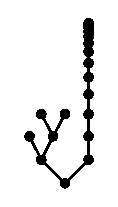
\includegraphics{img/Baum-nichtfundiert.pdf}
\caption{Baum ohne Fundierung\\ \phantom{Text}}
\label{fig:Baum-nichtfundiert}
\end{center}
\end{minipage}
\begin{minipage}[t]{0.45\textwidth}
\begin{center}
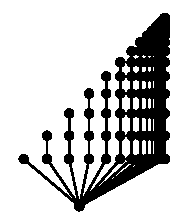
\includegraphics{img/Baum-fundiert.pdf}
\caption{Fundierter Baum\\ endloser Höhe}
\label{fig:Baum-fundiert}
\end{center}
\end{minipage}
\end{figure}

Bei einem Baum kann die Relation beispielsweise so definiert werden,
dass jeder der Knoten ausschließlich zu seinem Mutterknoten in Relation steht,
dergestalt dass man den Baum von der Wurzel aus herabsteigt. Die Abb.
\ref{fig:Baum-nichtfundiert} zeigt diesbezüglich einen Baum, der
einen endlosen Abstieg enthält. Dagegen zeigt Abb. \ref{fig:Baum-fundiert}
einen fundierten Baum. Obgleich dieses Exemplar von endloser Tiefe bzw.
Höhe ist, existiert kein endloser Abstieg.

\begin{Satz}
Ist $(M,<)$ wohlfundiert, existiert keine unendliche streng monoton
absteigende Kette, das heißt, es gilt die \emph{Descending Chain Condition}%
\index{Descending Chain Condition}
\[\lnot\exists f\in\Abb(\N,M)\colon \forall n\in\N\colon f(n+1)<f(n).\]
\end{Satz}
\begin{Beweis}
Angenommen, es läge eine unendlich absteigende Funktion $f$
vor. Da das Bild $f(\N)$ eine nichtleere Teilmenge von $M$ und $M$
wohlfundiert ist, muss ein minimales Element $y\in f(\N)$ existieren,
wozu ein $n$ mit $y=f(n)$ gehört. Nun wäre aber $f(n+1)<y$, was im
Widerspruch zur Minimalität von $y$ steht.\,\qedsymbol
\end{Beweis}

\begin{Satz}
Die Descending Chain Condition ist genau dann erfüllt, wenn jede
monoton absteigende Kette ab irgendeiner Stelle stabilisiert, das heißt,
\[\forall f\in\Abb(\N,M)\colon (\forall n\colon f(n+1)\le f(n))
\cond\exists m\colon\forall n\ge m\colon f(m)=f(n).\]
\end{Satz}
\begin{Beweis}
Es sei $f\colon\N\to M$ eine
beliebige Folge mit $f(n+1)\le f(n)$ für jedes $n$. Angenommen, $f$
enthielte unendlich viele Stellen $n_i$ mit $f(n_i+1)\ne f(n_i)$,
also $f(n_i+1)< f(n_i)$. Dann ließe sich die Teilfolge
$g\colon\N\to M$ mit $g(i):=n_i$ bilden, die der Descending
Chain Condition widerspricht. Ergo kann es von den Stellen $n_i$
nur endlich viele geben, womit die Folge $f$ ab einer Stelle
stabilisieren muss.

Zur Umkehrung. Angenommen, es läge $f$ mit $f(n+1)<f(n)$ für jedes $n$
vor. Für dieses $f$ gilt erst recht $f(n+1)\le f(n)$ für jedes $n$. Laut
Prämisse muss $f$ somit ab einem $m$ stabilisieren, womit $f(m+1)=f(m)$,
was im Widerspruch zur strengen Monotonie von $f$ steht.\,\qedsymbol
\end{Beweis}

\begin{Satz}[Wohlfundierte Induktion]%
\label{wf-Induktion}\index{wohlfundierte Induktion}%
\index{Induktion!wohlfundierte}\newlinefirst
Ist $(M,<)$ wohlfundiert, gilt für jede Teilmenge $A\subseteq M$ das Prinzip
\[(\forall x\in M\colon (\forall y\in M\colon y < x\cond y\in A)\cond x\in A)\cond A=M.\]
\end{Satz}
\begin{Beweis}
Dieser wird ganz analog zum dem von Satz \ref{Wohlordnungsprinzip}
auf S. \pageref{Wohlordnungsprinzip} geführt. Es ist genau
dann $A=M$, wenn das Komplement $B:=A^\compc=M\setminus A$ leer ist.
Man unternimmt die äquivalente Umformung
\begin{align*}
&B\ne\emptyset\cond (\exists x\in B\colon\lnot\exists y\in B\colon y<x)\\
\iff &(\forall x\in B\colon\exists y\in B\colon y<x)\cond B=\emptyset\\
\iff &(\forall x\in M\colon x\notin A\cond\exists y\in B\colon y<x)\cond A=M\\
\iff &(\forall x\in M\colon (\forall y\in B\colon \lnot y<x)\cond x\in A)\cond A=M.
\end{align*}
Und schließlich
\begin{align*}
(\forall y\in B\colon \lnot y<x)&\iff (\forall y\in M\colon y\notin A\cond\lnot y<x)\\
&\iff(\forall y\in M\colon y<x\cond y\in A).\,\qedsymbol
\end{align*}
\end{Beweis}
Da ausschließlich äquivalente Umformungen vorgenommen wurden, stellt sich
das Induktionsprinzip sogar als äquivalent zur Wohlfundiertheit
heraus.

Zu einer abstrakten Fassung des Induktionsprinzips findet man
folgendermaßen. Das Urbild
\[R^{-1}(y) := \{x\mid R(x,y)\} = \{x\mid x < y\}\]
nennt man auch das \emph{Anfangsstück} bis $y$ bezüglich $R$. Wir setzen
\[F(A) := \{x\mid R^{-1}(x)\subseteq A\}.\]
Nun mag das Induktionsprinzip formuliert werden als
\[\forall A\subseteq M\colon F(A)\subseteq A\cond A=M.\]
Eine Menge wollen wir diesbezüglich wieder \emph{induktiv} nennen, wenn
sie die Prämisse $F(A)\subseteq A$ erfüllt. Das Induktionsprinzip
besagt damit, dass jede induktive Menge mit $M$ übereinstimmen muss,
oder anders ausgedrückt, dass auf  $\mathcal P(M)$ keine anderen
Präfixpunkte von $F$ als $M$ selbst vorhanden sind.

\strong{Die gewöhnliche Induktion.}
Es ist $(\N,\prec)$ mit $n\prec m :\Leftrightarrow m=S(n)$ wohlfundiert,
wobei mit $S(n)$ wieder der Nachfolger von $n$ gemeint ist.
Als Induktionsprinzip erhält man hierbei die gewöhnliche Induktion.
Dies wird ersichtlich, wenn $\N$ in $\N=\{0\}\cup\N_{\ge 1}$ zerlegt
und daraufhin die allgemeine Äquivalenz
\[(\forall x\in A\cup B\colon E(x)) \Leftrightarrow
(\forall x\in A\colon E(x))\land (\forall x\in B\colon E(x))\]
herangezogen wird. Außerdem ergibt sich in diesem Fall
$R^{-1}(m) = S^{-1}(\{m\})$ als Anfangsstück. Die Prämisse des
Induktionsprinzips nimmt demnach die Form
\begin{align*}
F(A)\subseteq A \Leftrightarrow\; &(\forall m\in\{0\}\colon S^{-1}(\{m\})\subseteq A\cond m\in A)\,{\land}\\
&(\forall m\in\N_{\ge 1}\colon S^{-1}(\{m\})\subseteq A\cond m\in A)
\end{align*}
an. Die linke Seite der Konjuktion vereinfacht sich zu $0\in A$,
da $S^{-1}(\{0\})=\emptyset$ gilt, insofern $0$ keinen Vorgänger besitzt.
Auf der rechte Seite nutzt man
den Umstand aus, dass $m\in\N_{\ge 1}$ mit $\exists n\in\N\colon m=S(n)$
gleichbedeutend ist. Weil $S$ injektiv ist, ergibt sich nun
$S^{-1}(S(\{n\})) = \{n\}$, womit $S^{-1}(\{m\})\subseteq A$
äquivalent zu $n\in A$ ist. Ergo findet sich $n\in A\cond S(n)\in A$,
wobei dies für ein ganz allgemeines $n$ gelten muss, weil $m$ allgemein
gehalten war. Wem diese Umformungen zu unpräzise dargelegt sind, der mag
sie gerne zur Übung nochmals formal nachrechnen.

\strong{Die starke Induktion.}
Es ist $(\N,<)$ wohlfundiert, wobei mit $<$ die gewöhnliche Ordnung
auf $\N$ gemeint ist. Als Induktionsprinzip erhält man unmittelbar die starke
Induktion.

% #todo
% Ordinalzahlen. Eine Dominoreihe verläuft sich in einer Schachtel
% ins Unendliche. Der Stein mit Limesordinal muss extra umfallen,
% zu ihm gibt es keinen Vorgänger.

\section{Ordinalzahlen}

\subsection{Transfinite Induktion}

\begin{Satz}[Schema der transfiniten Induktion]%
\index{Induktion!transfinite}\newlinefirst
Für jede wohlgeordnete Menge $(M,<)$ und jede Eigenschaft $A(x)$ gilt
\[(\forall x\in M\colon (\forall y\in M\colon y<x\cond A(y))\cond A(x))
\cond (\forall x\in M\colon A(x)).\]
\end{Satz}
\begin{Beweis}
Weil jede wohlgeordnete Menge eine wohlfundierte ist, folgt der
Sachverhalt als Korollar aus Satz \ref{wf-Induktion}.\,\qedsymbol
\end{Beweis}

\noindent
Gleichwohl die Klasse der Ordinalzahlen eine echte ist, gilt das Prinzip
auch für sie. Insofern die Variablen $\alpha,\beta$ für Ordinalzahlen stehen
sollen, kürzen wir eine Formel der Form $\forall\alpha\in\mathrm{On}\colon A(\alpha)$
als $\forall\alpha\colon A(\alpha)$ ab. Das Schema nimmt diesbezüglich
die konzise Form%
\[(\forall\alpha\colon (\forall\beta < \alpha\colon A(\beta))
\cond A(\alpha))\cond (\forall\alpha\colon A(\alpha))\]
an. Zum Beweis der Prämisse kann diese in drei Teile aufgetrennt
werden, so wie die Prämisse der herkömmlichen Induktion in zwei
Teile, den Induktionsanfang und den Induktionsschritt, aufgetrennt wird.
Hier sind es
\[\begin{array}{@{}l@{\quad\;\;}l}
A(0), & \text{(Anfang)}\\[2pt]
\forall\alpha\colon A(\alpha)\cond A(\alpha+1), & \text{(Schritt auf den Nachfolger)}\\[2pt]
\forall\lambda\colon (\forall\beta<\lambda\colon A(\beta))\cond A(\lambda). & \text{(Schritt
aufs nächste Limes-Ordinal)}
\end{array}\]
Laut dem Fundierungsaxiom ist die Relation $\in$ auf der Klasse der
Mengen wohlfundiert. So ergibt das Schema der $\in$-Induktion,%
\index{Induktion!Epsilon-}%
\[(\forall x\colon (\forall y\in x\colon B(y))
\cond B(x))\cond (\forall x\colon B(x)).\]
Insofern $\beta<\alpha$ mit $\beta\in\alpha$ gleichbedeutend ist,
geht die transfiniten Induktion über die Ordinalzahlen also
aus der $\in$-Induktion hervor, indem man sich auf die Ordinalzahlen
beschränkt. Man braucht lediglich $B(x):=(x\in\mathrm{On}\cond A(x))$
setzen.

\subsection{Transfiniter Rekursionssatz}

Analog zu den natürlichen Zahlen gilt für Ordinalzahlen ein
Rekursionssatz,\index{Rekursionssatz!transfiniter} der es gestattet,
eine Funktion rekursiv für alle Ordinalzahlen zu definieren.

\subsection{Kumulative Hierarchie}

\begin{Definition}[Kumulative Hierarchie]%
\index{kumulative Hierarchie}\index{Hierarchie, kumulative}\newlinefirst
Man definiert $V_\alpha$ für Ordinalzahlen $\alpha$ rekursiv als
\begin{align*}
V_0 &:= \emptyset,\\
V_{\alpha+1} &:= \powerset(V_\alpha),\\
V_\lambda &:= {\textstyle\bigcup_{\alpha<\lambda} V_\alpha}.\qquad\text{($\lambda$ ein Limes-Ordinal)}
\end{align*}
\end{Definition}

\subsection{Grothendieck-Universen}

Die Systeme ZFC und NBG/MK sind mit einer störenden Beschränkung
behaftet, die freies Argumentieren unnötig einschränkt. Und zwar
mag die Vorstellung, dass man ein Universum\index{Universum} haben kann,
das alle denkbaren Mengen enthält, irrig sein. Stattdessen benötigen wir
anscheinend eine Hierarchie von Universen, so dass jedes Universum
wiederum Element eines Universums höherer Stufe sein wird. Es tun sich
nämlich die folgenden Probleme auf.

1. Als wir die russellsche Antinomie aus Satz \ref{Fixpunktsatz-Lawvere}
auf S. \pageref{Fixpunktsatz-Lawvere}, dem Fixpunktsatz von Lawvere
\index{Fixpunktsatz!von Lawvere} folgern wollten, wurde freies Argumentieren
dahingehend eingeschränkt, dass die Zusammenfassung $\Abb(X,Y)$ nicht zu
einer echten Klasse $X$ gebildet werden kann, da die Graphen der Abbildungen
echte Klassen sind, und somit nicht als Element einer Klasse auftreten dürfen.

2. Eine entsprechende Einschränkung tritt in der Kategorientheorie
auf. Dort mag es für gewisse Argumentationen außerdem erforderlich sein,
das Auswahlaxiom für ein größeres Universum verfügbar zu haben.
% #todo Zu schwammig. Ist damit das globale Auswahlaxiom gemeint?
% Außerdem gibt es noch andere Probleme, siehe Shulman 2008.

3. In der Typentheorie besteht ein Bedarf an einer gestuften
Hierarchie von Typuniversen. Will man Typen durch Mengen modellieren,
genügen Mengen und Klassen lediglich für die anfänglichen Stufen.

Statt nun ein etwaiges System für »Hyperklassen« zu ersinnen, greifen wir
auf das Konzept der Grothendieck"=Universen zurück, das diesen
Sachverhalt adäquat beschreibt.

\begin{Definition}[Grothendieck-Universum]\newlinefirst
Eine nichtleere Menge $U$ heißt \emph{Grothendieck-Universun},%
\index{Grothendieck-Universum} wenn
\[\begin{array}{@{}r@{\quad}l}
\text{(1)} & \forall x\in U\colon x\subseteq U,\\[2pt]
\text{(2)} & \forall x,y\in U\colon \{x,y\}\in U,\\[2pt]
\text{(3)} & \forall x\in U\colon\powerset(x)\in U,\\[2pt]
\text{(4)} & \forall I\in U\colon\forall x\in\operatorname{Abb}(I,U)\colon
  {\textstyle\bigcup_{i\in I}} x_i\in U.
\end{array}\]
\end{Definition}

\noindent
Die Grothendieck"=Universen stehen im engen Bezug zur kumulativen
Hierarchie. So ist $V_\lambda$ ein Grothendieck"=Universum, wenn
$\lambda$ nicht mehr mit Mengenoperationen von kleineren Ordinalzahlen
aus erreichbar ist. Das betrifft zunächst $V_\omega$ zur ersten unendlichen
Ordinalzahl $\omega$. Daraufhin kommt allerdings erst mit $V_\kappa$
wieder eines, wo $\kappa$ die nächste als Ordinalzahl betrachtete stark
unerreichbare Kardinalzahl ist. Im Folgenden wird näher darauf
eingegangen.

\begin{Satz}
Für jedes Limes-Ordinal $\lambda$ erfüllt $U:=V_\lambda$
die Axiome (1), (2), (3).
\end{Satz}
\begin{Beweis}
Zu (1). Es wird $\forall x\in V_\alpha\colon x\subseteq V_\alpha$ für jedes
Ordinal bestätigt per transfiniter Induktion über alle Ordinalzahlen.
Bei $\alpha=0$ gilt die Aussage trivial. Sie gelte für $\alpha$ als
Induktionsannahme IA. Zu folgern ist
\[\text{IA}, x\in V_{\alpha+1}\vdash x\subseteq V_{\alpha+1},\quad
\text{also}\;\;
\text{IA}, x\subseteq V_\alpha, u\in x\vdash u\subseteq V_\alpha.\]
Ist nun $u\in x$, so auch $u\in V_\alpha$, per Induktionsannahme
also $u\subseteq V_\alpha$.

Letztlich verbleibt für jedes Limes-Ordinal $\lambda$ zu bestätigen
\[(\forall \beta<\lambda\colon \forall x\in V_\beta\colon x\subseteq V_\beta),
x\in V_\lambda, u\in x\vdash u\in V_\lambda.\]
Mit $x\in V_\lambda$ existiert ein $\beta<\lambda$ mit $x\in V_\beta$,
und somit $x\subseteq V_\beta$. Mit $u\in x$ erhält man daraufhin
$u\in V_\beta$. Ergo existiert $\beta<\lambda$ mit $u\in V_\beta$,
womit $u\in V_\lambda$ gilt.

Zu (2). Mit $x,y\in V_\lambda$ liegen ein $\alpha<\lambda$ mit
$x\in V_\alpha$ und ein $\beta<\lambda$ mit $y\in V_\beta$ vor. Bezüglich
$\gamma:=\max(\alpha,\beta)$ gilt dann $x,y\in V_\gamma$,
ergo $\{x,y\}\subseteq V_\gamma$. Man hat $\gamma+1<\lambda$ mit
$\{x,y\}\in V_{\gamma+1}$, womit $\{x,y\}\in V_\lambda$.

Zu (3). Mit $x\in V_\lambda$ liegt ein $\alpha<\lambda$ mit $x\in V_\alpha$ vor.
Wie zuvor gezeigt, folgt $x\subseteq V_\alpha$, und somit
$\powerset(x)\subseteq\powerset(V_\alpha)$, also $\powerset(x)\in
\powerset(\powerset(V_\alpha)=V_{\alpha+2}$. Mit $\beta:=\alpha+2$ existiert
daher ein $\beta<\lambda$ mit $\powerset(x)\in V_\beta$, womit
$\powerset(x)\in V_\lambda$.\,\qedsymbol
\end{Beweis}
